\documentclass[openright]{report}
\makeatletter\@twosidetrue\makeatother
\usepackage[fixlanguage]{babelbib}
\usepackage[spanish,mexico]{babel}
\usepackage[utf8]{inputenc}
\usepackage[T1]{fontenc}
\usepackage{vmargin}
\usepackage{enumitem}
\usepackage[hidelinks]{hyperref}
\usepackage{pdfpages}
\usepackage[nottoc]{tocbibind}
\usepackage{textcomp}
\usepackage{amssymb}
\usepackage{dsfont}
\usepackage{float}
\usepackage{listings}
\usepackage{listingsutf8}
\usepackage{appendix}
\usepackage{minted}
\usepackage{array}
\usepackage{caption}
\usepackage{tikz}
\usepackage{tikz-uml}
\usetikzlibrary{arrows.meta,
                matrix,
                positioning,
                automata, 
                decorations.pathreplacing
                }
\usepackage{skak}
\usepackage{xcolor}
%\usepackage{svg}
\usepackage{amsmath}
\usepackage[noabbrev, spanish]{cleveref}
\usepackage{tcolorbox}
\tcbuselibrary{listings,skins}
\usepackage[chapter, Algoritmo]{algorithm}
\usepackage[noend]{algpseudocode}
\usepackage{lineno}
\usepackage{parcolumns}
\usepackage{fancyhdr}
\usepackage[multiple]{footmisc}
\pagestyle{fancy}
\fancyhf{}
\fancyhead[L]{\rightmark}
\fancyhead[R]{\thepage}
\renewcommand{\headrulewidth}{0pt}

% Cosas que hay que quitar:
%\linenumbers
%\usepackage{draftwatermark}
%\SetWatermarkText{VERSIÓN SINODALES}
%\SetWatermarkHorCenter{0.6\paperwidth}
%\SetWatermarkVerCenter{0.56\paperheight}
%\SetWatermarkScale{2}
% Ya no hay que quitar nada

\usepackage{amsthm}
\theoremstyle{definition}
\newtheorem{definition}{Definición}[section]

\newcolumntype{C}{>$c<$}

\definecolor{bg}{HTML}{D3D3D3}
\definecolor{darkgreen}{rgb}{0.18,0.54,0.34}
\definecolor{red}{rgb}{1,0,0}

\tcbuselibrary{listingsutf8,minted}
\tcbset{listing utf8=inputenc}


\lstdefinestyle{mybash}
{language=bash,
keywordstyle=\color{blue},
basicstyle=\ttfamily,
morekeywords={peter@kbpet},
alsoletter={:~},
morekeywords=[2]{python},
keywordstyle=[2]{\color{red}},
literate=*{\$}{{{\color{red}\$}}}{1} 
         {:}{{{\color{red}:}}}{1}
         {\{}{{{\color{black}\{}}}{1},
}

\lstset{style=mybash}

\newtcblisting{commandshell}{
%colback=white,
%colupper=black,
colframe=black,
listing only,
listing style=mybash,
listing options={
	style=mybash,
	numberstyle=\tiny\color{black}}
}

\newtcblisting{commandshellwhite}{colback=purple!5,colupper=black,colframe=purple!5,
listing only,listing remove caption=true,listing options={language=sh, name=Listado}}

\newtcblisting{pythonshell}{listing engine=minted, minted language=python,colback=white,colupper=black,colframe=white!75!black,
listing only,listing remove caption=true,listing options={name=Listado}}

\newtcblisting{pythonshellnoframe}{listing engine=minted, minted language=python,colback=white,colupper=black,colframe=white,
listing only,listing remove caption=true,listing options={name=Listado}}


\newenvironment{code}{\captionsetup{type=listing}}{}
\captionsetup[listing]{name=Listado}
%every listing line={\textcolor{green}{\small\ttfamily\bfseries DeathStar \$> }
\renewcommand\lstlistingname{Listado}
\lstset{
    escapeinside={(*@}{@*)},          % if you want to add LaTeX within your code
}

\definecolor{rojo}{RGB}{255,0,0}
\definecolor{verde}{RGB}{0,255,0}
\definecolor{azul}{RGB}{0,0,255}
\definecolor{naranja}{RGB}{255,69,0}
\definecolor{dorado}{RGB}{255,125,0}
\definecolor{morado}{RGB}{128,0,128}
\definecolor{acian}{RGB}{0,255,255}
\definecolor{misol}{RGB}{255,255,0}
\definecolor{minegro}{RGB}{0,0,0}
\definecolor{mimorado}{RGB}{241,101,244}
\usetikzlibrary{matrix}
\makeatletter
\newcounter{qrr@tikz@omino}
\newcounter{qrr@tikz@omino@up}
\newcounter{qrr@tikz@omino@right}
\tikzset{
    omino/.style={/tikz/omino/.cd,#1},
    omino/distance/.initial=1,
    omino/radius/.initial=.5,
    omino/at/.style={/tikz/shift={(#1)}},
    omino/rotate/.style={/tikz/rotate=#1},
    omino/s/.code=
        \setcounter{qrr@tikz@omino}{0}%
        \setcounter{qrr@tikz@omino@up}{0}%
        \setcounter{qrr@tikz@omino@right}{0}%
        \pgfkeysalso{/tikz/insert path={(0,0) node[/tikz/omino/nodes/.try,/tikz/omino/node normal/.try,/tikz/omino/node start/.try] {\qrr@tikz@omino@text@start}}},
    omino/u/.code=%
        \stepcounter{qrr@tikz@omino}%
        \stepcounter{qrr@tikz@omino@up}%
        \pgfkeysalso{/tikz/insert path={
            to[/tikz/omino/how] ++(up:#1)
            node[/tikz/omino/nodes/.try,/tikz/omino/node normal/.try,/tikz/omino/node up/.try]{\qrr@tikz@omino@text@up}}},
    omino/d/.code=%
        \stepcounter{qrr@tikz@omino}%
        \addtocounter{qrr@tikz@omino@up}{-1}%
        \pgfkeysalso{/tikz/insert path={
            to[/tikz/omino/how] ++(down:#1)
            node[/tikz/omino/nodes/.try,/tikz/omino/node normal/.try,/tikz/omino/node down/.try]{\qrr@tikz@omino@text@down}}},
    omino/l/.code=%
        \stepcounter{qrr@tikz@omino}%
        \addtocounter{qrr@tikz@omino@right}{-1}%
        \pgfkeysalso{/tikz/insert path={
            to[/tikz/omino/how] ++(left:#1)
            node[/tikz/omino/nodes/.try,/tikz/omino/node normal/.try,/tikz/omino/node left/.try]{\qrr@tikz@omino@text@left}}},
    omino/r/.code=%
        \stepcounter{qrr@tikz@omino}%
        \stepcounter{qrr@tikz@omino@right}%
        \pgfkeysalso{/tikz/insert path={
            to[/tikz/omino/how] ++(right:#1)
            node[/tikz/omino/nodes/.try,/tikz/omino/node normal/.try,/tikz/omino/node right/.try] {\qrr@tikz@omino@text@right}}},
    omino/u/.default=\pgfkeysvalueof{/tikz/omino/distance},
    omino/d/.default=\pgfkeysvalueof{/tikz/omino/distance},
    omino/l/.default=\pgfkeysvalueof{/tikz/omino/distance},
    omino/r/.default=\pgfkeysvalueof{/tikz/omino/distance},
    omino/how/.style=,
    omino/reset/.code=
        \pgfutil@in@_{#1}%
        \ifpgfutil@in@
            \qrr@tikz@omino@split#1\relax
        \else
            \edef\pgf@tempa{\csname qrr@tikz@omino@coords@#1\endcsname}%
            \expandafter\qrr@tikz@omino@split\pgf@tempa\relax
        \fi
        \pgfkeysalso{/tikz/insert path={(omino-n-#1.center) node[/tikz/omino/nodes/.try, /tikz/omino/node reset/.try] {\qrr@tikz@omino@text@reset}}},
    omino/do/.code={\@tfor\@next:=#1\do{\pgfkeysalso{/tikz/omino/\@next}}},
    omino/node reset/.style={draw=none,fill=none},
    omino/node normal/.style={
        name=omino-n-\number\c@qrr@tikz@omino,
        alias=omino-n-\number\c@qrr@tikz@omino@right_\number\c@qrr@tikz@omino@up,
        omino/@store coords
    },
    omino/@store coords/.code=
        \expandafter\xdef\csname qrr@tikz@omino@coords@\arabic{qrr@tikz@omino}\endcsname
        {\number\c@qrr@tikz@omino@right_\number\c@qrr@tikz@omino@up},
    omino/Text/.code 2 args=\expandafter\edef\csname qrr@tikz@omino@text@#1\endcsname{#2},
    omino/Text={up}{},omino/Text={down}{},omino/Text={left}{},omino/Text={right}{},omino/Text={start}{},omino/Text={reset}{}
}
\def\qrr@tikz@omino@split#1_#2\relax{\setcounter{qrr@tikz@omino@right}{#1}\setcounter{qrr@tikz@omino@up}{#2}}

\tikzset{
    omino/x mirror/.style={/tikz/cm={-1,0,0,1,(0,0)}},
    omino/y mirror/.style={/tikz/cm={1,0,0,-1,(0,0)}}
}

\tikzset{fun/.code={\pgfmathtruncatemacro\@fun{\number\c@qrr@tikz@omino/4*100}\pgfkeysalso{fill=blue!\@fun!red}}}
\makeatother
\tikzset{
    tetris/.style={/tikz/tetris/.cd,#1},
    tetris/1/.style={/tikz/omino={do=suuu}},
    tetris/2/.style={/tikz/omino={do=suur}},
    tetris/6/.style={/tikz/omino={do=suul}},
    tetris/3/.style={/tikz/omino={do=suru}},
    tetris/7/.style={/tikz/omino={do=sulu}},
    tetris/4/.style={/tikz/omino={do=surd}},
    tetris/8/.style={/tikz/omino={do=s}},
    tetris/9/.style={/tikz/omino={do=s}},
    tetris/0/.style={/tikz/omino={do=s}},
    tetris/5/.style={/tikz/omino={s,u,u,reset=1,r}}
}
\makeatletter

\makeatother
\newcommand*{\thesamepictureeverywhere}{\matrix[column sep=.5cm, row sep=.5cm, ampersand replacement=\&] {
\path [tetris=1];  \&
\path [tetris=6]; \& 
\path [tetris=2]; \&
\path [tetris=3];  \& 
\path [tetris=7]; \&
\path [tetris=4];  \&
\path [tetris=8]; \&
\path [tetris=9];  \&
\path [tetris=0];  \&
\path [tetris=5];\\};}

\tikzset{
    tetris/1/.prefix style={/tikz/omino/nodes/.append style={fill=rojo,text=white}},
    tetris/2/.prefix style={/tikz/omino/nodes/.append style={fill=azul}},
    tetris/6/.prefix style={/tikz/omino/nodes/.append style={fill=acian}},
    tetris/3/.prefix style={/tikz/omino/nodes/.append style={fill=verde}},
    tetris/7/.prefix style={/tikz/omino/nodes/.append style={fill=dorado}},
    tetris/4/.prefix style={/tikz/omino/nodes/.append style={fill=naranja}},
    tetris/8/.prefix style={/tikz/omino/nodes/.append style={fill=misol}},
    tetris/9/.prefix style={/tikz/omino/nodes/.append style={fill=mimorado}},
    tetris/0/.prefix style={/tikz/omino/nodes/.append style={fill=minegro}},
    tetris/5/.prefix style={/tikz/omino/nodes/.append style={fill=morado}},
    omino/Text={start}{.}
}


\newenvironment{lcases}
  {\left.\begin{aligned}}
  {\end{aligned}\left\lbrace}

\bibliographystyle{babplain}

\pdfminorversion=5
\setpapersize{USletter}
\setmarginsrb{3.2cm}{2cm}{3.2cm}{2cm}{1cm}{1cm}{1cm}{1cm}

\renewcommand{\lstlistingname}{Listado}

\begin{document}


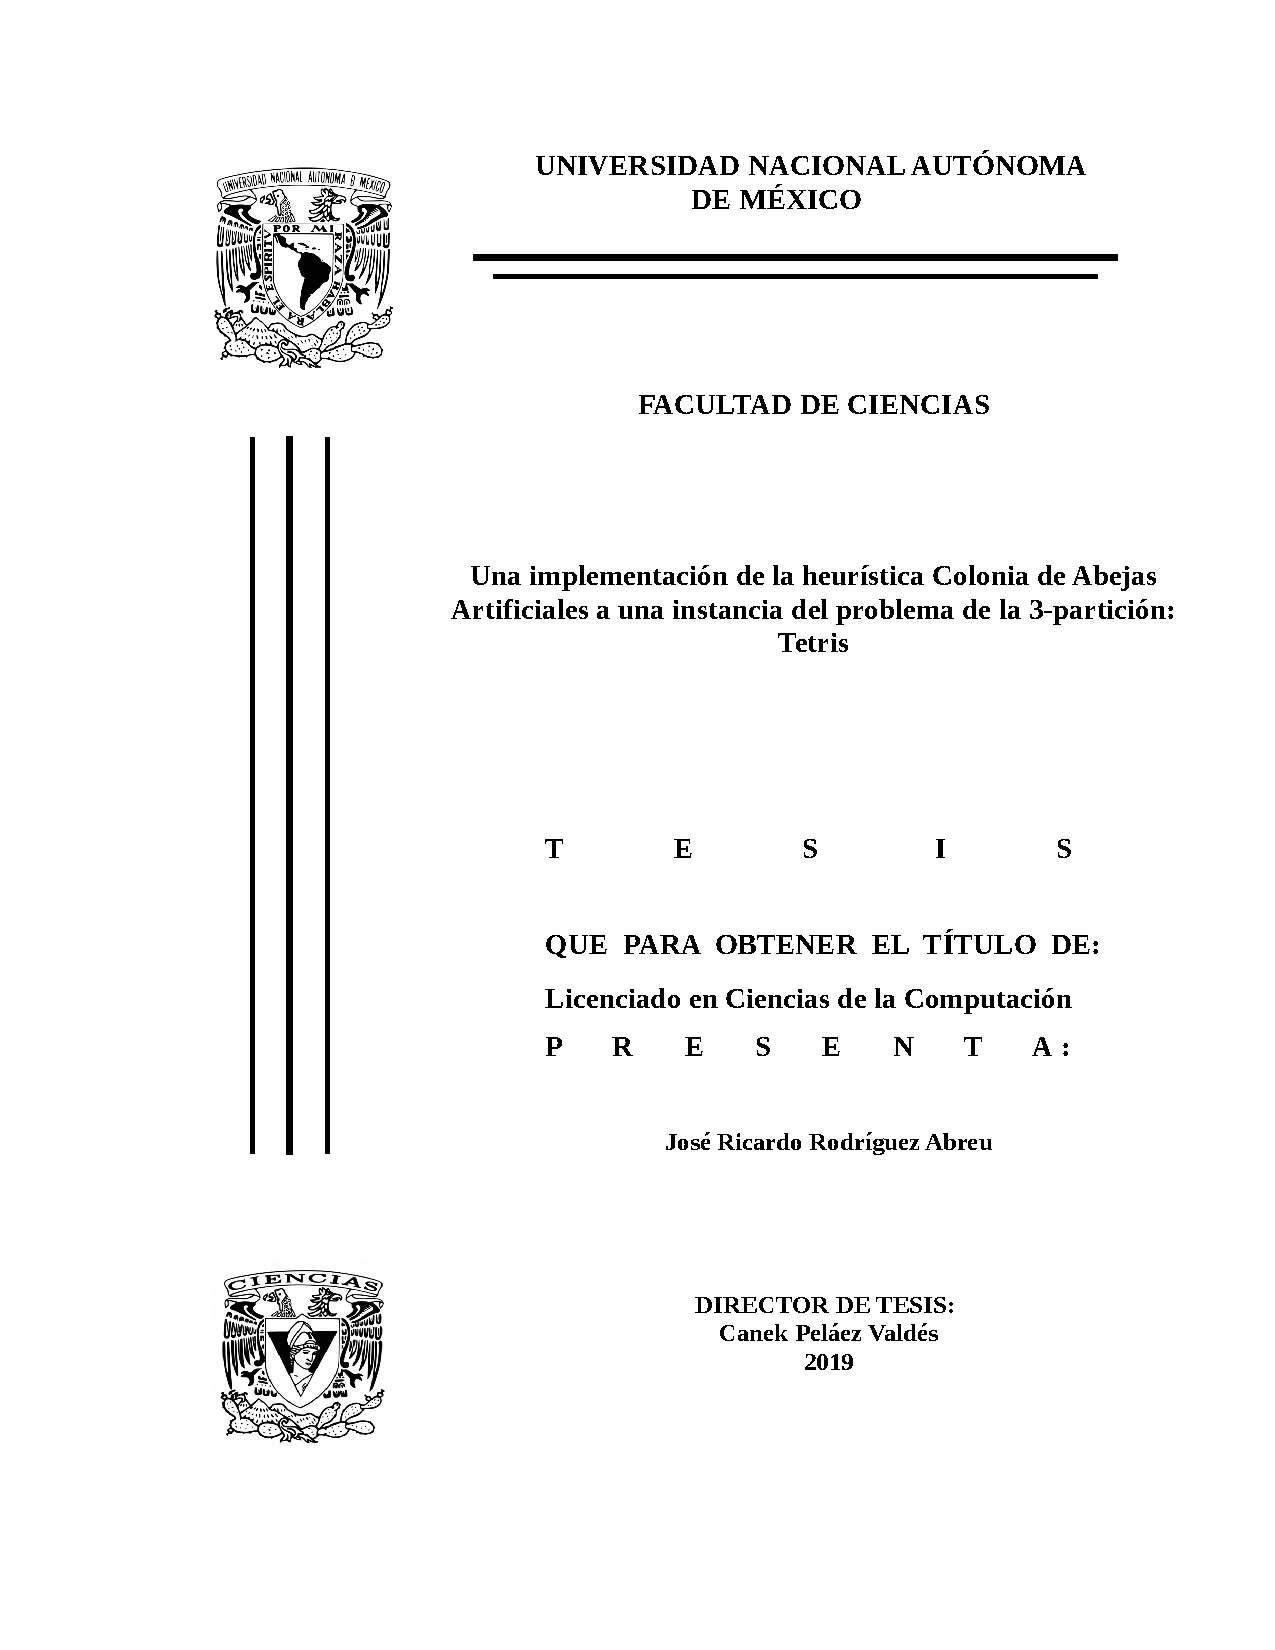
\includepdf[pages=1,noautoscale=true,offset=50 -80]{portada/Portada_no_dr}

\pagenumbering{Roman} 

\begin{center}
{\large \textbf{Hoja de Datos del Jurado:}}
\end{center}
\begin{enumerate}

\item Datos del alumno \\
Rodríguez \\
Abreu \\
José Ricardo \\
5526542430 \\
Universidad Nacional Autónoma de México \\
Facultad de Ciencias \\
Ciencias de la Computación \\
309216139 

\item Datos del tutor \\
Dr \\
Canek \\
Peláez \\
Valdés \\

\item Datos del sinodal 1 \\
Dra \\
Adriana \\
Ramírez \\
Vigueras \\

\item Datos del sinodal 2 \\
Dr \\
David Guillermo \\
Romero \\
Vargas \\

\item Datos del sinodal 3 \\
Dr \\
José de Jesús \\
Galaviz \\
Casas \\

\item Datos del sinodal 4 \\
M en C \\
Manuel Cristóbal \\
López \\
Michelone \\

\item Datos del trabajo escrito \\
Una implementación de la heurística Colonia de Abejas Artificiales a una instancia del problema de la 3-partición: Tetris \\
136 p \\
2019 
\end{enumerate} 
\newpage
\chapter*{Agradecimientos}
\pagenumbering{Roman} 

Mis padres Elia y Edgar que con su inagotable amor y con su ejemplo, siempre me impulsaron y enseñaron a superarme día a día. 

A mis hermanos Luis y Mauricio que siempre han sido sinónimo de apoyo y estabilidad. Sin su sacrificio yo no estaría aquí. 

A mi hermana Susana quién fue mi cómplice en más de una ocasión y siempre me ha brindado amor incondicional, gracias.

Gracias a mi tutor Canek Peláez Valdés a quien siempre le estaré eternamente agradecido por su guía, asesoría y dedicación a este trabajo. 

A Karla Ramírez Pulido, por su paciencia, enseñanza y amistad en cada uno de los años que trabajamos juntos. 

También quiero agradecer a José de Jesús Galaviz Casas por haberme recibido en la universidad y haberme  mostrado que el crecimiento intelectual y personal siempre debe venir acompañado de humildad y responsabilidad científica. 

Quiero agradecer de manera muy particular a Roberto Monroy Argumedo porque gracias a su apoyo incondicional y preocupación casi paternal hacia mi formación, fue que pude construir las bases sobre  las que puedo asentar mi futuro. Descanse en paz. 

Agradezco a todos mis profesores que a través de las aulas, dentro y fuera de la UNAM, aportaron en mi persona para mi desarrollo académico. 

Por último quiero agradecer a la Universidad Nacional Autónoma de México y a la Facultad de Ciencias por brindarme todas las herramientas necesarias para una educación de calidad. De corazón, \textit{¡Goya!}

\newpage
\clearpage

\pagenumbering{arabic}

\tableofcontents

\setcounter{secnumdepth}{3}
\setcounter{tocdepth}{3}

\chapter{Introducción}

Desde el inicio del uso de las computadoras y el uso de la \textit{Máquina de
  Turing} como modelo de cómputo, uno de los principales objetivos ha sido el
tratar de resolver problemas de manera automatizada. A partir de la década de
los años cuarentas del siglo pasado y en pleno apogeo de la segunda guerra
mundial, los programadores afrontaron la gran complicación de usar un enfoque
para no orientar a las máquinas a calcular todos los posibles resultados sino
disminuir el número de operaciones. Por aquella tormentosa época, matemáticos y
criptógrafos no tuvieron opción más que reducir el espacio de búsqueda de sus
problemas para optimizar el tiempo de ejecución de sus (muy) limitadas
máquinas. Al reducir el espacio de búsqueda contribuyeron a encontrar soluciones
de una manera más eficiente~\cite{GalavizCasas}.

El modelo computacional que actualmente se usa puede resolver problemas
cotidianos de manera bastante eficiente, como son mostrar la letra de una canción en
uno de los buscadores más usado y más famoso~\cite{Harikumar}. Esta afirmación
parte de la idea de que existen problemas que son fáciles de entender pero
difíciles o imposibles de hacer que una computadora dé una respuesta;
está demostrado que problemas como \textit{The Halting problem}
\footnote{La función \texttt{HALT} toma de entrada un par $\langle \alpha, x
\rangle$ y regresa $1$ sí y sólo si la máquina de Turing $M_{\alpha}$ se
detiene dada la entrada $x$, en un número finito de pasos.} no pueden
ser resueltos por una máquina de Turing.
Existen incógnitas que pueden ser fácilmente enunciables como \textit{¿es $N$ un número
primo?}\footnote{Problema del número compuesto.} o \textit{¿puede una persona
recorrer $K$ lugares de forma eficiente sin repetir ninguno y al finalizar
regresar al lugar de origen?}\footnote{Problema del agente viajero.} pero al ser programadas,
pueden tardar años en ser solucionados por una máquina si no se les da
herramientas correctas de resolución~\cite{arora2009computational}.

Para todos aquellos problemas en los cuales crear un algoritmo y esperar
una solución óptima no es posible, ya sea por su complejidad o porque
simplemente no se sabe si existe un algoritmo eficiente, se usan otros métodos
que aunque posiblemente no sean los óptimos, nos ayudan a dar soluciones que
surgen con el objetivo de ser lo más efectivas posibles~\cite{Pearl1984}.
Algunas de las compañías de software de uso cotidiano y masivo, empresas tan
conocidas como de transporte\cite{uber-heuristic} o comercio electrónico
\footnote{Conocido como \textit{e-commerce}, incluye empresas como Uber,
Amazon, Netflix, Google, entre otras.}, han usado estas
alternativas como recurso para mejorar su impacto en el mercado\cite{Linden} \cite{Smith2017}.

Dada una problemática bien definida y que se pueda probar que exista 
dentro de la clase de complejidad
\textsl{NP}-completo o \textsl{NP}-duro y una heurística de optimización
combinatoria como las definidas en ~\cite{Pearl1984}, ¿cómo comparar si la
solución propuesta es buena?  Una forma es desarrollar la aplicación de la
heurística al problema y analizar los resultados obtenidos. Para analizar las
soluciones se deberá definir un objetivo a conseguir con los 
datos de entrada y un comportamiento que encuentre una solución 
al problema definido. De esta manera, se podría observar que los resultados son
eficiente al menos en algún punto de la ejecución.

El objetivo principal de este trabajo es tomar el problema de calcular los
posibles desenlaces de un juego de Tetris y seleccionar una serie de
movimientos adecuados, usando una heurística de solución genérica que realice
optimización combinatoria como la mencionada en~\cite{karaboga2005idea}.

Se usará la heurística de nombre \textit{Colonia de Abejas Artificiales} como
método de cálculo para los posibles desenlaces de cada iteración del problema.
La heurística consiste en dividir la búsqueda de posibles soluciones óptimas
usando la reducción del espacio con la ayuda de distintas estrategias que se
basan en las tácticas de un ente natural: conductas como el de
reducir el lugar geográfico de una colonia de abejas para localizar fuentes
de alimentos y mejorar el comportamiento de un panal.
El propósito de usar esta heurística es adaptar una función de costo que
se desarrollará sobre el contexto del juego de Tetris.

Se ha elegido como problema el juego de Tetris por las interesantes
conclusiones que se han obtenido del trabajo
en~\cite{DBLP:journals/corr/cs-CC-0210020} y por
la familiaridad que presenta para una gran cantidad de personas, por lo que
entender sus reglas y lógica no conlleva un reto mayor al del propósito del
presente trabajo. Los objetivos a optimizar por la heurística son: maximizar
el número de filas eliminadass mientras la computadora juega; maximizar el
número de piezas colocadas al finalizar el juego; maximizar el número de veces
que se realiza un ``tetris'' (que es cuando se eliminan simultáneamente cuatro
líneas); y minimizar la altura de la fila más alta en cualquier momento
durante el juego.

En el capítulo dos se hablará de diferentes tipos de problemas computacionales,
terminando con la explicación de un problema \textsl{NP}-completo que será el
punto de partida para explicar el problema a tratar en esta tesis;
Tetris, que será abordado en el capítulo cuatro y la solución a usar
será descrita en el capítulo tres. Tanto en el capítulo cinco como en el seis se
discutirá el ambiente y la implementación del problema mientras que en el siete
los resultados del desempeño de la solución propuesta. Para finalizar este
trabajo, las conclusiones se presentan en el capítulo ocho.

%%% Local Variables:
%%% mode: latex
%%% TeX-master: "../main"
%%% End:


\chapter{Problemas \textsl{NP}-completos y \textsl{NP}-duros}


Si bien la palabra \textit{computación} ha existido por cientos 
de años, fue hasta que su significado cambió 
que hizo necesario generar una clasificación de problemas. 
Se mostrará que la clasificación por clases de problemas fue una consecuencia 
natural temprana y se enuncian las definiciones de dichas clases.

\section{Historia y definición}
\label{sec:np-def}

A principios del siglo XX, en agosto de 1900 se llevó acabo el segundo
congreso internacional de matemáticas en París, Francia.
Motivado por el congreso y la llegada de un nuevo siglo, el matemático
David Hilbert planteó un conjunto de veintitrés problemas de lo que él llamó
``el futuro problema de las matemáticas''.
Para 1902, Hilbert mantenía un optimismo sobre la resolución de sus problemas,
diciendo: \textit{For in mathematics there is no ignorabimus!} [Para las matemáticas
no existe el \emph{ignorabimus}\footnote{La palabra \textit{ignorabimus} a la que
Hilbert hace referencia, tiene origen en un latinismo que dice
\textit{Ignoramus et ignorabimus} y significa  ``desconocemos y
desconoceremos''.}]~\cite{Grattan-Guinness}. Veintiocho años más tarde y aunque
Hilbert no lo incluyó en su lista de veintitrés problemas originales, enunció
otro para la comunidad matemática: crear un algoritmo que tome como entrada
un predicado (con un número finito de axiomas y enunciados) y regrese como
resultado ``Sí'' o ``No'' si es universalmente válido. Este problema es conocido
como el \textit{Entscheidungsproblem} o el problema de
decisión~\cite{hilbert1950principles}. En otras palabras, el problema de
decisión consiste en averiguar si existe un algoritmo genérico que decida
si una fórmula de cálculo de primer orden es un teorema.

En el año 1936, el matemático Alan Turing publicó un artículo que
revolucionó e impactó al mundo y a las matemáticas; de nombre \textit{
Sobre los números computables, con una aplicación al problema de decisión}
\footnote{El título original es \textit{On computable numbers, with an
application to the Entscheidungsproblem}.}; en este trabajo Turing
definió \textit{una máquina de cómputo} después denominada como \textit{
máquina de Turing} y una \textit{máquina de cómputo universal}. De forma
paralela y del otro lado del océano Atlántico, Alonso Church publicó su trabajo
llamado en inglés \textit{An Unsolvable Problem of Elementary Number Theory},
donde de manera independiente pero casi simultanea a Turing, trabajó sobre
el \emph{Entscheidungsproblem} usando el modelo llamado \textit{cálculo
lambda}~\cite{church1935unsolvable}. Años más tarde, Alan Turing y Alonso Church
trabajarían juntos para formular la equivalencia de sus modelos~\cite{sep-church-turing}.

La máquina de Turing o MT es un modelo matemático de una computadora hipotética
la cual usa un conjunto predefinido de reglas para determinar el resultado de
un conjunto de variables de entrada\footnote{\cite{gurovich2015introduccion}
define formalmente a una máquina de Turing como un 7-tuplo $M=(Q,\Sigma, \Gamma,
\delta, q_{0}, \square,F)$.}. La máquina de cómputo universal o \textit{Máquina
de Turing universal} es una máquina que puede calcular cualquier secuencia
computable dada una descripción de una máquina de Turing $M$. La máquina universal $U(M)$
puede realizar exactamente los mismos cálculos de $M$.

En ese mismo artículo Alan Turing, además de plantear el \emph{Entscheidungsproblem}
usando su máquina de Turing y la máquina universal para demostrar que el
planteamiento de Hilbert era falso, Turing usa el proceso de diagonalización para
mostrar que no se puede construir un proceso que tome la descripción general de
una MT y nos diga si es libre de ciclos (\textit{circle-free}) o terminará su
ejecución; este problema se le conoce como \textit{El problema del paro} o
\textit{The Halting Problem}. Con estos resultados Alan Turing crea una primera
clasificación de problemas para las MT: los problemas computables y los no
computables~\cite{Turing1936}.

Posterior a esta primera clasificación, hubo la necesidad de seguir dividiendo
los problemas desde el punto de vista de otra restricción que presentan las MT.
Desde el inicio del uso de las primeras computadoras electrónicas, se
descubrió que el modelo básico de las máquinas de Turing fallan al considerar
la cantidad de tiempo o memoria que necesita una computadora real, un
problema crítico en la actualidad pero más aún en aquellos primeros días de
la computación moderna. La idea clave para medir el tiempo y el espacio en función
de la longitud de la entrada llegó a principio de la década de los sesentas,
por Juris Hartmanis y Richard Stearns cuyo artículo \textit{Sobre la complejidad
computacional de los algoritmos}\footnote{\textit{On the Computational
Complexity of Algorithms} es el título original.} sentó las bases de lo que
se conoce como complejidad computacional~\cite{Hartmanis1965}.

Al principio de la teoría, las investigaciones giraban en torno a
sólo tratar de entender éstas nuevas formas de medición y cómo se
relacionaban entre ellas. En los sesentas también se menciona por primera vez el
término de \textit{clases de complejidad} y se genera un concepto de eficiencia
computacional al medir el tamaño de la entrada con polinomios~\cite{Fortnow2002}.

Para entender las distintas \textit{clases de complejidad} y antes de enunciar
las definiciones formales de \textsl{P}, \textsl{NP}, \textsl{NP}-completo y
\textsl{NP}-duro, se enunciará un ejemplo que puede ser útil para entender la
dificultad de los cálculos que realizan las máquinas para encontrar soluciones
de algoritmos no triviales: suponer que existe un gran grupo de estudiantes
en los que se necesita que trabajen en equipo para un proyecto, se sabe qué
estudiantes se llevan bien entre sí y se desea colocar a los estudiantes en
equipos en los que todos se lleven bien. Es deseable que los equipos sean con la menor cantidad de
integrantes, dos de ser posible y así todos los estudiantes realicen alguna
parte del proyecto. Una forma de encontrar la solución sería calcular todos los
posibles equipos y descartar los que tienen personas que no se lleven 
bien entre sí; pero para una muestra de 40 estudiantes, podrían existir más de
300 mil trillones de posibles equipos (las combinaciones que forman particiones
del conjunto potencia de estudiantes). Este programa se le llama \textit{Mínimo
  apareamiento maximal}~\cite{10.1007/978-3-540-79228-4_32}.  En 1965, Jack
Edmonds describió un algoritmo eficiente para resolver el problema de
emparejamiento y sugirió una definición formal de \textit{eficiencia
  computacional} \cite{Mathematics}. La clase de problemas con soluciones
eficientes (o polinomiales) sería luego renombrada como la clase \textsl{P}\footnote{Viene del
  inglés \textit{Polynomial Time}.}. En 1960 Jack Edmonds dijó que un problema es fácil 
  de resolver si el tiempo está limitado por un polinomio en el tamaño de su representación 
  (en la clase \textsl{P})~\cite{Schrijverpolyhedralcombinatorics}.

Para muchos problemas parecidos y relacionados no se conoce un algoritmo
eficiente que pueda resolverlos: regresando al ejemplo de los estudiantes, ¿cuál
sería el algoritmo si ahora se hacen grupos de al menos tres? (partición de triángulos)
¿Qué pasa si se quiere sentar a los estudiantes en una mesa redonda sin que sean
vecinos de algún alumno incompatible? (Ciclo Hamiltoniano) ¿Y si se ponen a los
estudiantes en tres grupos y que cada estudiante se encuentre en un grupo sólo
con personas compatibles? (3-coloración).  Todos estos problemas tienen en común
que dada una posible solución, se puede corroborar que sea correcta en un tiempo
eficiente.  La colección de problemas que tienen soluciones verificables en
tiempo eficiente es conocida como la clase \textsl{NP}\footnote{Viene del inglés
  \textit{ Nondeterministic Polynomial-Time}.}.

En 1971 Stephen Cook y Leonid Levin hicieron la demostración que lleva sus
apellidos, en la que prueban que cualquier problema \textsl{NP} puede
ser \textit{reducido} en tiempo polinomial por una máquina de Turing
determinista a un problema en específico. El concepto
(mas no el término) de \textsl{NP}-completez fue presentado por primera
vez en~\cite{Cook}.
En la demostración del trabajo Cook-Levin, los autores muestran el
\textit{Problema de satisfacibilidad booleana}, también conocido como
\texttt{\textbf{SAT}}, como el primer problema \textsl{NP}-completo (aunque posteriormente 
demuestran otros como \textbf{3-SAT}).
\texttt{SAT} consiste en determinar si una fórmula booleana con variables y sin cuantificadores es o
no satisfacible; en otras palabras, si existe
alguna asignación de valores para sus variables que haga a la expresión
verdadera.

Formalmente se dice que si $\varphi$ es una fórmula booleana con
variables $u_{1}, u_{2}, \ldots, u_{n}$ y $z \in \{0,1\}^{n}$, entonces
$\varphi(z)$ denota el valor de $\varphi$ cuando a las variables de $\varphi$
le son asignados los valores de $z$. Una fórmula $\varphi$ es satisfacible si
existe una asignación $z$ tal que $\varphi(z)$ sea verdadera. Si no existe
$z$ para $\varphi(z) = \texttt{TRUE}$, se dice que $\varphi$ es
insatisfacible~\cite{arora2009computational}. Sólo un año después de la
demostración, en su artículo \textit{Reducibility Among Combinatorial Problems} el computólogo
Richard M. Karp, usó las conclusiones del trabajo para definir 21 problemas
\textsl{NP}-completos adicionales~\cite{Karp1972}.

Para poder enunciar las definiciones formales de las clases \textsl{P} y \textsl{NP},
se necesita conocer al menos tres definiciones relacionadas previamente:
lenguaje decidible, la clase \texttt{DTIME} y reductibilidad. Las siguientes
siete definiciones formales son tomadas de~\cite{arora2009computational}:



\theoremstyle{definition}
 \begin{definition}
  Se dice que una máquina decide un lenguaje $L \subseteq \{0, 1\}^{*}$ si
 calcula la función $f_{L}:\{0,1\}^{*} \longrightarrow \{0,1\}$, donde
 $f_{L} (x) = 1 \Leftrightarrow x \in L$.
\end{definition}

 \theoremstyle{definition}
 \begin{definition}
  Sea $T: \mathbb{N} \longrightarrow \mathbb{N}$
 alguna función. Un lenguaje \textsl{L} es elemento de \texttt{DTIME}$(T(n))$ si y sólo
 si existe alguna máquina de Turing que corra en tiempo $c \cdot T(n)$ para alguna
 constante $c > 0$ y que decida $L$.
 \end{definition}

 \theoremstyle{definition}
 \begin{definition}
Un lenguaje $L \subseteq \{0,1\}^{*}$ es polinonialmente \textbf{reducible} a
un lenguaje $L' \subseteq \{0,1\}^{*}$ (también llamado
\textit{Karp reducible}), denotado por $L \leq_{p} L'$, si existe una
función computable en tiempo polinomial
$f : \{0,1\}^{*} \longrightarrow \{0,1\}^{*}$ tal que para cada
$x \in \{0,1\}^{*}$, $x \in L$ si y sólo si $f(x) \in L'$.
 \end{definition}

\noindent
Dadas las definiciones anteriores y el ejemplo mencionado, se pueden enunciar las
definiciones formales de las clases \textsl{P} y \textsl{NP} y el resto de las
clases de complejidad:

 %theoremstyle{definition}
 %begin{definition}
  %setcounter{enumi}{3}

 \theoremstyle{definition}
 \begin{definition}
 Se define a la clase \textsl{P} como
  $\textsl{P} = \cup_{c \geq 1} ~ \texttt{DTIME}(n^{c})$.
   \end{definition}

 \theoremstyle{definition}
 \begin{definition}
Un lenguaje $L \subseteq \{0, 1\}^{*}$ está en \textsl{NP} si existe un
  polinomio $p: \mathbb{N} \longrightarrow \mathbb{N}$ y una máquina de Turing $M$
  que se ejecute en tiempo polinomial (llamada la verificadora de $L$) tal
  que para cada $x \in \{0,1\}^{*}$,
\end{definition}

  \begin{displaymath}
    x \in L \Leftrightarrow \exists u \in \{0,1\}^{p(|x|)},~
    \textrm{tal que} ~ M(x,u) = 1.
  \end{displaymath}

 \theoremstyle{definition}
 \begin{definition}
  Se dice que $L'$ es \textsl{NP}-duro o \textsl{NP}-\textit{hard} si
  $L \leq_{p} L'$ para cada $L \in \textsl{NP} $.
  \end{definition}

 \theoremstyle{definition}
 \begin{definition}
 Se dice que $L'$ es \textsl{NP}-completo si $L'$ es \textsl{NP}-duro y
  $L' \in \textsl{NP}$.
    \end{definition}




\section{3-Partición}
\label{sec:3-particion}

El problema de \texttt{3-PARTITION} o 3-Partición es un problema \textsl{NP}-completo,
el cual enuncia que dado un conjunto finito $\mathcal{A}$ de $3m$ elementos,
una cota $b \in \mathds{Z}^{+}$ y una ``medida''\footnote{El autor usa la
palabra \textit{``size''} como alternativa a una mejor palabra para la función.}
$s(a) \in \mathds{Z}^{+}$ con $a \in \mathcal{A}$, tal que
satisfaga que $b/4 < s(a) < b/2$ y que $\sum_{a \in \mathcal{A}} s(a) = m \cdot b$,
¿puede $\mathcal{A}$ ser particionado en $m$ conjuntos disjuntos $S_{1}, S_{2},
S_{3}, \ldots , S_{m}$ tal que para cada $1 \leq i \leq m $, $\sum_{a \in S_{i}}
s(a)=b$? En otras palabras, dado un conjunto de $N$ elementos,
¿puede encontrarse una partición de $N/3$ subconjuntos tal que la suma de los
elementos de cada uno debe ser la misma y la cardinalidad de cada subconjunto
debe ser tres?

La definición de 3-partición junto con la demostración
de su \mbox{\textsl{NP}-completez} apareció en el año de 1979 y es visto como
un problema de decisión~\cite{Garey:1990:CIG:574848}. Para la demostración de la
\textsl{NP}-completez del problema se usa una reducción del problema de la
4-partición, el cual es \textsl{NP}-completo y previamente demostrado a partir
del problema general de la partición
(\Cref{fig:secuenciaNP}). 3-partición es un problema de los llamados
\textit{totalmente o fuertemente \textsl{NP}-completos}, esto quiere decir que
sigue siendo \textsl{NP}-completo incluso cuando los enteros (o elementos) de
$\mathcal{A}$ están acotados por un polinomio en función de la longitud de la entrada.

\begin{figure}[h]
\centering
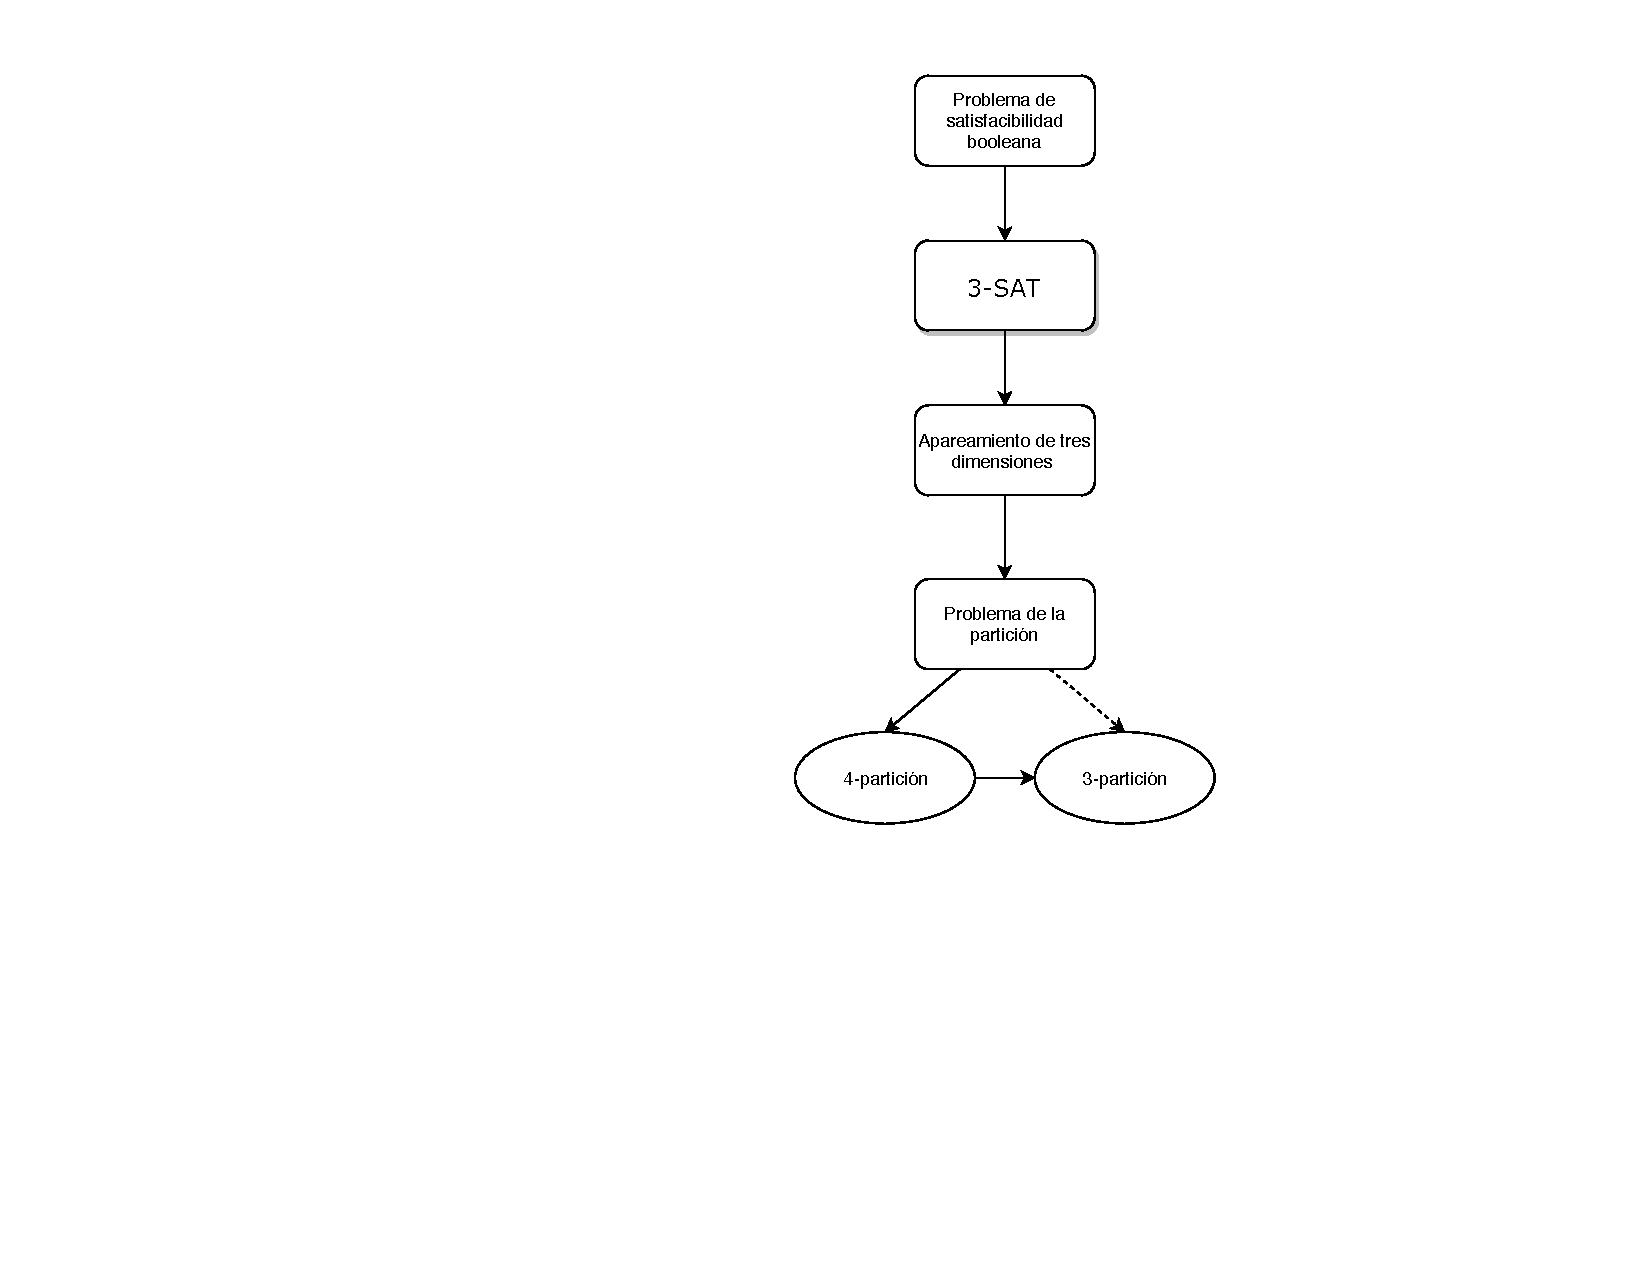
\includegraphics[width=.45\textwidth,keepaspectratio,trim={12cm 6cm 7cm 0cm}]{./images/2_2_1.pdf}
\caption{Diagrama de la secuencia de las transformaciones usadas para
probar que 3-partición es \textsl{NP}-completo.}
\label{fig:secuenciaNP}
\end{figure}

Este trabajo se encuentra íntimamente relacionado al problema y clasificación de
la 3-partición debido al resultado de la \textit{fuerte \textsl{NP}-completez};
esta propiedad será de utilidad cuando se tenga que explicar la simplificación de
una representación unaria del problema a implementar, como se discutirá en el
\cref{chap:cuatro}. Varias afirmaciones posteriores parten del hecho de que
hay una reducción de la 3-partición por lo que no se sabe si existe un método de
resolución eficiente al problema presentado en esta tesis.

%%% Local Variables:
%%% mode: latex
%%% TeX-master: "../main"
%%% End:


\cleardoublepage

\chapter{Heurística: Colonia de Abejas Artificiales}

Una fuerte característica del ser humano es su forma de proceder 
para resolver problemas. En las Ciencias de la Computación, 
la problemática de encontrar una respuesta incluye el camino de 
describir la forma de resolverlo. En este capítulo se abordan algunas formas de 
hacer que la computadora ejecute dicho camino y se discute una descripción 
que se implementa como método de solución.

\section{Algoritmos}

Suponga que una persona va al supermercado y crea una lista con todos los
productos de su carrito. Cada producto tiene asociado un precio y se desea
averiguar si el total del carrito es menor o igual a la cantidad de dinero
disponible para efectuar la compra. ¿Cuál sería un método de solución
adecuado para este problema? Aunque pareciera que el problema es muy fácil
de resolver, el nivel de detalle que deben tener las indicaciones y pasos asociados a
la solución, posiblemente no son triviales de enunciar para una persona que nunca
ha descrito estos procesos a una computadora:

\begin{itemize}

\item \textbf{Input:} $L = $ Una lista de números que representan el precio de
  cada producto y un número $N$ el cual representa el límite de gastos.

\item \textbf{Output:} Un valor booleano de \texttt{TRUE} si la suma de los
  valores del carrito es menor o igual al número $N$, \texttt{FALSE} en caso
  contrario.

\end{itemize}

\begin{algorithm}
  \begin{algorithmic}[1]
    \Procedure{SumaMenorQue}{$L$, $N$}
      \State $N \leftarrow N -$ \textsc{SacaPrimero}($L$)
      \While{\textbf{true}}
        \If{$N < 0$}
          \State \textbf{return false}
        \EndIf
        \If{\textsc{EsVacio($L$)}}
          \State \textbf{return true}
        \EndIf
        \State $N \leftarrow N -$ \textsc{SacaPrimero}($L$)
      \EndWhile
    \EndProcedure
  \end{algorithmic}
  \caption{Algoritmo \textsc{SumaMenorQue}.}
  \label{code:algoritmo}
\end{algorithm}

Para llegar a la solución de un problema, una persona utiliza muchas veces
el instinto que va desarrollando a los largo de los años para analizar,
atacar y ejecutar un proceso que da una solución. Si se intenta
transmitir dicha técnica a una computadora, la manera más fácil de realizarlo
es mediante un proceso llamado \textit{algoritmo}.
Se puede decir informalmente que un algoritmo es cualquier procedimiento bien
definido que toma algún valor, o conjunto de valores como entrada
(o \textbf{Input}) y produce algún valor, o conjunto de valores como
salida (u \textbf{Output})~\cite{Cormen}. El análisis del problema en conjunto
a la abstracción de los objetos asociados y el resultado, producen
una serie de instrucciones que si se siguen correctamente, bajo una entrada
$I$, siempre regresará una salida $O$.

La investigación sobre la formalización de la definición de la palabra
\textit{algoritmo} sigue siendo motivo de estudio hasta nuestros días~\cite{Buss}.
Debido a los distintos tipos de problemas a resolver, existen muy diferentes
procesos, entradas y salidas que se pueden producir. Muchas veces existe más
de un algoritmo para resolver el mismo problema y algunos de ellos producen una
salida de manera más óptima que otros\footnote{En este caso, el factor para
que un algoritmo es más eficiente que otro se basa en la complejidad
en espacio o tiempo (\textit{big-O}).} . La llamada ``caracterización'' de los algoritmos
es algo que se ha discutido por más de doscientos años; un ejemplo de esto
es el algoritmo de la criba de Eratóstenes que nos permite hallar todos los
números primos menores a un número natural $m$ dado.

Para propósitos de esta tesis, la definición informal que se usará será la
siguiente: \textbf{Un algoritmo es una secuencia de pasos bien definida y finita
  tal que dada una entrada $I$, produce siempre la salida $O$}. Se considerará
que los algoritmos deben tener también la característica de finitud
(\cite{Physics},~\cite{Rogers1967}~y~\cite{Cormen}).

Así como existen problemas en los que escribir el algoritmo para encontrar
la solución resulta sencillo y el proceso descrito pueda verse fácilmente
eficiente (como el~\Cref{code:algoritmo}), existen problemas en los que
dar la descripción para obtener la mejor solución no es una opción práctica.

\subsection{\texttt{3-SAT}}

Sea el problema \texttt{3SAT}, el cual consiste en dado un conjunto de fórmulas
$\phi = \{x_{1}, x_{2}, x_{3}, ..., x_{n}\}$ con cada $x_{i}$ una fórmula lógica
de la forma $x_{i} = p_{i} \lor q_{i} \lor r_{i} $, con $ p_{i}, q_{i}, r_{i}$,
variables o términos lógicos, se deberá encontrar una
interpretación $\mathcal{I}$ tal que $\mathcal{I}(\phi) = \mathcal{I}(x_{i}) = 1$
$\forall i \in \{1,2,...,n\}$. Existen algoritmos para resolver este problema
y similares\footnote{Recordar que en el capítulo 2 se aborda la equivalencia de
los problemas \textsl{NP}-completos.}, sin embargo, su complejidad en tiempo es de la
forma $O(X^{n})$ con $3|\phi| = n$ y $X$ una constante~\cite{Marques-Silva}.

Para propósitos demostrativos, se ha creado un algoritmo de búsqueda exhaustiva.
El código que se encuentra en el \cref{apendice:sat} sirve para correr
ejemplos de fórmulas y encontrar interpretaciones en las que el valor de
verdad de la fórmula sea \texttt{TRUE} (o~1). En caso de que no exista una
interpretación verdadera, el programa implementado regresa el mensaje de que no se pudo
realizar una asignación (lo que sería equivalente al valor de \texttt{FALSE} en \texttt{3-SAT}):

\begin{figure}[h]
\begin{displaymath} 
\mathcal{I}(s \lor j \lor \neg z) =\left\{
  \begin{array}{rcl}
    \mathcal{I}(s) & = & \texttt{FALSE} \\
    \mathcal{I}(j) & = & \texttt{FALSE}  \\
    \mathcal{I}(z) & = & \texttt{FALSE} 
  \end{array}
  \right.
\end{displaymath}
\caption[short caption]{Salida del programa en el \cref{apendice:sat}.}
\label{fig:salida1}
\end{figure} 

Se puede ver que $\mathcal{I}(\phi) = 1$ con la asignación de la \Cref{fig:salida1} 
ya que $\mathcal{I}(z) = 0 \rightarrow \mathcal{I}(\neg z) = 1$ y
por lo tanto, $\mathcal{I}(s \lor j \lor \neg z) = 1$.

Con este mismo programa se puede forzar una fórmula que no tenga solución y así
realizar el cálculo de todas las posibles combinaciones de asignaciones.
Si se agrega  como parámetro \texttt{--no-solucion}, el programa agregará el
siguiente conjunto $\phi_{imp}$ de cláusulas al programa, definido en \Cref{tab:3sat}.

\begin{table}[h]
\[
\small
\centering
\begin{array}{C|C|C|C|C|C|C}
$P$ & $Q$ & $R$ & $\overbrace{(P \lor Q \lor R)}^{\textbf{(a)}}$ & $\overbrace{(\neg P \lor Q \lor R)}^{\textbf{(b)}}$ & $\overbrace{(P \lor \neg Q \lor R)}^{\textbf{(c)}}$ & $\overbrace{(P \lor Q \lor \neg R)}^{\textbf{(d)}}$  \\
\hline
T & T & T & T & T & T & T \\
T & T & F & T & T & T & T \\
T & F & T & T & T & T & T \\
T & F & F & T & F & T & T \\
F & T & T & T & T & T & T \\
F & T & F & T & T & F & T \\
F & F & T & T & T & T & F \\
F & F & F & F & T & T & T
\end{array}
\]

\[
\small
\centering
\begin{array}{C|C|C|C|C|C|C}
$P$ & $Q$ & $R$ & $\overbrace{(\neg P \lor \neg Q \lor R)}^{\textbf{(e)}}$ & $\overbrace{(\neg P \lor Q \lor \neg R)}^{\textbf{(f)}}$ & $\overbrace{(P \lor \neg Q \lor \neg R)}^{\textbf{(g)}}$ & $\overbrace{(\neg P \lor \neg Q \lor \neg R)}^{\textbf{(h)}}$  \\
\hline
T & T & T & T & T & T & F \\
T & T & F & F & T & T & T \\
T & F & T & T & F & T & T \\
T & F & F & T & T & T & T \\
F & T & T & T & T & F & T \\
F & T & F & T & T & T & T \\
F & F & T & T & T & T & T \\
F & F & F & T & T & T & T
\end{array}
\]
\caption{Tabla de verdad con las fórmulas de todas las posibles combinaciones de tres variables $P$, $Q$ y $R$ en la forma normal conjuntiva \textit{(NFC)}.\label{tab:3sat}}
\end{table}

Como se puede observar en la tabla \Cref{tab:3sat}, existe siempre para alguna
combinación de valores de $P$, $Q$ y $R$, el valor de $F$ (o falso) en todas
las columnas y filas, por lo tanto, como se ve en la tabla \ref{tab:3sat2}, se puede
suponer que $\nexists~\mathcal{I} \mid \mathcal{I}(\phi_{imp}) = 1$.

\begin{table}
\[
\centering
\begin{array}{C|C|C|C}
$P$ & $Q$ & $R$ & $ (a) \land (b)  \land (c)  \land (d)  \land (e)  \land (f)  \land (g)  \land (h)  $  \\
\hline
T & T & T & F \\
T & T & F & F \\
T & F & T & F \\
T & F & F & F \\
F & T & T & F \\
F & T & F & F \\
F & F & T & F \\
F & F & F & F
\end{array}
\]
\caption{Tabla de verdad con las conjunciones del resultado de la
tabla \Cref{tab:3sat}.} \label{tab:3sat2}
\end{table}

\begin{center}
  \begin{minipage}{1.0\textwidth}
    \begin{lstlisting}[caption={Ejecución de una fórmula sin solución.}\label{code:3sat-no-solucion1},captionpos=b]
      (*@
      \begin{commandshell}
        # python sat.py --no-solucion
        No se pudo realizar asignación, se intentó 1 fórmula(s).
        Num de asignaciones que se realizaron: 14
      \end{commandshell}
      @*)
    \end{lstlisting}
  \end{minipage}
\end{center}


Al no existir una posible combinación para este conjunto de fórmulas, el
algoritmo en el~\cref{apendice:sat} asignará todas las posibles combinaciones de
valores a cada una de las variables; para tres variables el número de
asignaciones que se realizan es 14, que es el resultado de la suma del total de las
llamadas recursivas y es el número total de aristas en el árbol de búsqueda. El
hecho de que el árbol sea binario depende sólo de que existan dos posibles valores
de verdad para cada variable.

\begin{figure}[H]
\centering
\begin{tikzpicture}[level/.style={sibling distance=60mm/#1}]
  \node (a) {$P$}
    child {node (b) {$Q$}
      child {node (d) {$R$}
      	child {node (dl) {$\mathcal{I}(\phi)$}}
      	child {node (dr) {$\mathcal{I}(\phi)$}}
      	}
      child {node (e) {$R$}
      	child {node (el) {$\mathcal{I}(\phi)$}}
      	child {node (er) {$\mathcal{I}(\phi)$}}
      	}
    }
    child {node (c) {$Q$}
    child {node (f) {$R$}
    	child {node (fl) {$\mathcal{I}(\phi)$}}
    	child {node (fr) {$\mathcal{I}(\phi)$}}
    	}
      child {node (g) {$R$}
      	child {node (gl) {$\mathcal{I}(\phi)$}}
      	child {node (gr) {$\mathcal{I}(\phi)$}}
      	}
    }; 	
%\path (a) -- (b) node {TRUE};
\path (a) edge node[above=3pt]{$1$} (b);
\path (a) edge node[above=3pt]{$0$} (c);

\path (b) edge node[left]{$1$} (d);
\path (b) edge node[right]{$0$} (e);
\path (c) edge node[left]{$1$} (f);
\path (c) edge node[right]{$0$} (g);

\path (d) edge node[left]{$1$} (dl);
\path (d) edge node[right]{$0$} (dr);
\path (e) edge node[left]{$1$} (el);
\path (e) edge node[right]{$0$} (er);
\path (f) edge node[left]{$1$} (fl);
\path (f) edge node[right]{$0$} (fr);
\path (g) edge node[left]{$1$} (gl);
\path (g) edge node[right]{$0$} (gr);
\end{tikzpicture}
\caption{Árbol de asignaciones de valores con tres variables.} \label{fig:a3sat01}
\end{figure}

Para una cláusula con tres variables, el árbol realiza 14 asignaciones, para
dos cláusulas con seis variables el árbol tendrá 126 aristas representando
las asignaciones, para tres claúsulas $1,022$ y para 21 variables el número se eleva
a $4,194,302$. Para 33 variables (u once cláusulas) se corrió el programa durante más de
un día debido a que el árbol es demasiado grande para revisar todas las asignaciones en
menos de 24 horas\footnote{Se realizó la experimentación y se hizo el total de 
asignaciones en 26 horas con 25 minutos y 41 segundos.}\footnote{El número obtenido fue $17,179,869,182$ (diecisiete mil
ciento setenta y nueve millones ochocientos sesenta y nueve mil ciento ochenta
y dos).}.

\begin{figure}[h]
% GNUPLOT: LaTeX picture
\setlength{\unitlength}{0.240900pt}
\ifx\plotpoint\undefined\newsavebox{\plotpoint}\fi
\sbox{\plotpoint}{\rule[-0.200pt]{0.400pt}{0.400pt}}%
\begin{picture}(1500,900)(0,0)
\sbox{\plotpoint}{\rule[-0.200pt]{0.400pt}{0.400pt}}%
\put(171.0,131.0){\rule[-0.200pt]{4.818pt}{0.400pt}}
\put(151,131){\makebox(0,0)[r]{$0$}}
\put(1419.0,131.0){\rule[-0.200pt]{4.818pt}{0.400pt}}
\put(171.0,313.0){\rule[-0.200pt]{4.818pt}{0.400pt}}
\put(151,313){\makebox(0,0)[r]{$500$}}
\put(1419.0,313.0){\rule[-0.200pt]{4.818pt}{0.400pt}}
\put(171.0,495.0){\rule[-0.200pt]{4.818pt}{0.400pt}}
\put(151,495){\makebox(0,0)[r]{$1,000$}}
\put(1419.0,495.0){\rule[-0.200pt]{4.818pt}{0.400pt}}
\put(171.0,677.0){\rule[-0.200pt]{4.818pt}{0.400pt}}
\put(151,677){\makebox(0,0)[r]{$1,500$}}
\put(1419.0,677.0){\rule[-0.200pt]{4.818pt}{0.400pt}}
\put(171.0,859.0){\rule[-0.200pt]{4.818pt}{0.400pt}}
\put(151,859){\makebox(0,0)[r]{$2,000$}}
\put(1419.0,859.0){\rule[-0.200pt]{4.818pt}{0.400pt}}
\put(171.0,131.0){\rule[-0.200pt]{0.400pt}{4.818pt}}
\put(171,90){\makebox(0,0){$2$}}
\put(171.0,839.0){\rule[-0.200pt]{0.400pt}{4.818pt}}
\put(488.0,131.0){\rule[-0.200pt]{0.400pt}{4.818pt}}
\put(488,90){\makebox(0,0){$3$}}
\put(488.0,839.0){\rule[-0.200pt]{0.400pt}{4.818pt}}
\put(805.0,131.0){\rule[-0.200pt]{0.400pt}{4.818pt}}
\put(805,90){\makebox(0,0){$4$}}
\put(805.0,839.0){\rule[-0.200pt]{0.400pt}{4.818pt}}
\put(1122.0,131.0){\rule[-0.200pt]{0.400pt}{4.818pt}}
\put(1122,90){\makebox(0,0){$5$}}
\put(1122.0,839.0){\rule[-0.200pt]{0.400pt}{4.818pt}}
\put(1439.0,131.0){\rule[-0.200pt]{0.400pt}{4.818pt}}
\put(1439,90){\makebox(0,0){$6$}}
\put(1439.0,839.0){\rule[-0.200pt]{0.400pt}{4.818pt}}
\put(171.0,131.0){\rule[-0.200pt]{0.400pt}{175.375pt}}
\put(171.0,131.0){\rule[-0.200pt]{305.461pt}{0.400pt}}
\put(1439.0,131.0){\rule[-0.200pt]{0.400pt}{175.375pt}}
\put(171.0,859.0){\rule[-0.200pt]{305.461pt}{0.400pt}}
\put(30,495){\rotatebox{90}{\makebox(0,0){Asignaciones}}
}\put(805,29){\makebox(0,0){Fórmulas}}
\put(488,136){\usebox{\plotpoint}}
\multiput(488.00,136.58)(3.894,0.498){79}{\rule{3.193pt}{0.120pt}}
\multiput(488.00,135.17)(310.373,41.000){2}{\rule{1.596pt}{0.400pt}}
\multiput(805.58,177.00)(0.500,0.514){631}{\rule{0.120pt}{0.511pt}}
\multiput(804.17,177.00)(317.000,324.939){2}{\rule{0.400pt}{0.256pt}}
\put(488,136){\makebox(0,0){$+$}}
\put(805,177){\makebox(0,0){$+$}}
\put(1122,503){\makebox(0,0){$+$}}
\put(1122.0,503.0){\rule[-0.200pt]{0.400pt}{85.760pt}}
\put(171.0,131.0){\rule[-0.200pt]{0.400pt}{175.375pt}}
\put(171.0,131.0){\rule[-0.200pt]{305.461pt}{0.400pt}}
\put(1439.0,131.0){\rule[-0.200pt]{0.400pt}{175.375pt}}
\put(171.0,859.0){\rule[-0.200pt]{305.461pt}{0.400pt}}
\end{picture}

\caption[short caption]{Muestra del crecimiento de asignaciones respecto a las fórmulas de $\phi$.}
\label{fig:satfigure}
\end{figure} 


El algoritmo dado produce la solución (si es que existe) pero el costo en tiempo
es demasiado alto. Este algoritmo es lo que se le denomina de tiempo ``exponencial'' y
esto se debe a que el número de asignaciones crece de la siguiente manera (\Cref{fig:satfigure}):

\begin{figure}[H]
\centering
\begin{tikzpicture}[level/.style={sibling distance=50mm/#1}]
\node [circle,draw] (z){$\varphi_{1}$}
  child {node [circle,draw] (a) {$\varphi_{2}$}
    child {node [circle,draw] (b) {$\varphi_{3}$}
      child {node (p1) {$\vdots$}
        child {node [circle,draw] (d) {$\varphi_{n}$}}
        child {node [circle,draw] (e) {$\varphi_{n}$}}
      }
      child {node (p2) {$\vdots$}}
    }
    child {node [circle,draw] (g) {$\varphi_{3}$}
      child {node (p3) {$\vdots$}}
      child {node (p4) {$\vdots$}}
    }
  }
  child {node [circle,draw] (j) {$\varphi_{2}$}
    child {node [circle,draw] (k) {$\varphi_{3}$}
      child {node (p5) {$\vdots$}}
      child {node (p6) {$\vdots$}}
    }
  child {node [circle,draw] (l) {$\varphi_{3}$}
    child {node (p7) {$\vdots$}}
    child {node (c){$\vdots$}
      child {node [circle,draw] (o) {$\varphi_{n}$}}
      child {node [circle,draw] (p) {$\varphi_{n}$}
        child [grow=right] {node (q) {$=$} edge from parent[draw=none]
          child [grow=right] {node (q) {$O(2^{n})$} edge from parent[draw=none]
            child [grow=up] {node (r) {$\vdots$} edge from parent[draw=none]
              child [grow=up] {node (s) {$O(2^{3}=8)$} edge from parent[draw=none]
                child [grow=up] {node (t) {$O(2^{2}=4)$} edge from parent[draw=none]
                  child [grow=up] {node (u) {$O(2^{1})=2$} edge from parent[draw=none]}
                }
              }
            }
            child [grow=down] {node (v) {$O\left(\displaystyle\sum_{i = 1}^n 2^n \right)$}edge from parent[draw=none]}
          }
        }
      }
    }
  }
};
\path (a) -- (j) node [midway] {+};
\path (b) -- (g) node [midway] {+};
\path (k) -- (l) node [midway] {+};
\path (k) -- (g) node [midway] {+};
\path (d) -- (e) node [midway] {+};
\path (o) -- (p) node [midway] {+};
\path (o) -- (e) node (x) [midway] {$\cdots$};
\path (q) -- (r) node [midway] {+};
\path (s) -- (r) node [midway] {+};
\path (s) -- (t) node [midway] {+};
\path (s) -- (l) node [midway] {=};
\path (t) -- (u) node [midway] {+};
\path (z) -- (u) node [midway] {=};
\path (j) -- (t) node [midway] {=};
\path (q) -- (v) node [midway] {=};



\path (z) edge node[above=3pt]{$1$} (a);
\path (z) edge node[above=3pt]{$0$} (j);

\path (a) edge node[left]{$1$} (b);
\path (a) edge node[right]{$0$} (g);
\path (j) edge node[left]{$1$} (k);
\path (j) edge node[right]{$0$} (l);

\path (b) edge node[left]{$1$} (p1);
\path (b) edge node[right]{$0$} (p2);
\path (g) edge node[left]{$1$} (p3);
\path (g) edge node[right]{$0$} (p4);
\path (k) edge node[left]{$1$} (p5);
\path (k) edge node[right]{$0$} (p6);
\path (l) edge node[left]{$1$} (p7);
\path (l) edge node[right]{$0$} (c);

\path (p1) edge node[left]{$1$} (d);
\path (p1) edge node[right]{$0$} (e);
\path (c) edge node[left]{$1$} (o);
\path (c) edge node[right]{$0$} (p);

\end{tikzpicture}
\caption{Posibles valores de verdad por cada variable en un árbol binario.} \label{fig:a3sat02}
\end{figure}

En el 2010 se publicó un artículo donde describen un algoritmo que reduce la
complejidad a $O(1.439^{n})$ y existe una competencia anual que premia a las
mejores implementaciones para encontrar soluciones al problema
\texttt{SAT},\cite{Kutzkov2010} \cite{satcompetition}, sin embargo las
soluciones siguen siendo exponenciales.  Habría que mencionar que si se
encuentra una solución en tiempo \textsl{P} se estaría demostrando que
$\textsl{P}=\textsl{NP}$.

\section{Heurísticas}

Una alternativa a solucionar problemas como \texttt{3-SAT} o
equivalentes\footnote{Que sea un problema perteneciente a la clase \textsl{NP} o
  con una cota \textit{$big-O$} que se quisiera reducir.} son estrategias y procesos
que se utilizan fácilmente debido a la información libremente aplicada para
controlar los procesos de resolución de problemas en máquinas. Estos procesos
son criterios, métodos o principios para decidir cuál de los varios cursos de
acción alternativos promete ser el más eficaz para lograr algún objetivo. Estos
procesos reciben el nombre de \textbf{heurísticas}~\cite{Pearl1984}.

A diferencia de los algoritmos\footnote{En algunos textos, 
como~\cite{DeInformatica2010} las heurísticas son llamadas 
\textit{algoritmos heurísticos}.} informalmente definidos previamente, las
heurísticas también son una secuencia de pasos bien definida pero dada una
entrada $I$, produce una salida $o \in \texttt{OUTPUT}$ con $\texttt{OUTPUT}$ un
conjunto de posibles valores de solución.  Las respuestas dadas por las
heurísticas normalmente no suelen ser la mejor solución, pero intentan producir
una solución \emph{suficientemente buena}~\cite{Gigerenzer2008}.  Generalmente
sus salidas son el resultado de ejecuciones de funciones estocásticas y
raramente almacenan información del proceso de obtención del resultado
previo~\cite{heuristicdefoxford},\cite{Pearl1984}.

Las heurísticas son tan diversas que es difícil clasificarlas exclusivamente en sólo 
una categoría, sin embargo existen características que comparten ciertas heurísticas:
los métodos resolutivos llamados de \textit{búsqueda tabú} son aquellos que determinan 
una posible respuesta, las marcan y premian la exploración de soluciones alejadas de las 
posibles respuestas marcadas. Los algoritmos (heurísticos) genéticos están por su parte 
inspirados en la evolución biológica, modificando poblaciones (de objetos a mejorar) y 
premiando a las soluciones más cercanas al objetivo. Existen muchos otras heurísticas como 
las redes neuronales o reocido simulado y si bien todas diferentes, comparten la 
característica de producir soluciones sin garantizar necesariamente que sea la mejor.

Cuando se habla de heurísticas, es importante mencionar que en algunos
textos~\cite{Pearl1984} hablan sobre una cierta \textit{intuición} o criterio
cuando se refiere al plantearlas como métodos resolutivos, por
los que en algunas ocasiones es difícil entender el \textit{``¿por qué
  funciona?''}; se propone que la intuición mencionada es la capacidad de hacer
predicción sobre un conjunto de datos o la eliminación de información previa
innecesaria (o ``ruido'')~\cite{Gigerenzer2008}.

\subsection{El problema de las 8 reinas}

Franz Nauck publicó en 1850 un (ahora) famoso problema para el matemático Gauss:
el problema consiste en obtener el método para determinar cómo ocho reinas
pueden ser colocadas en un tablero de ajedrez\footnote{El problema general es
  colocar $n$ reinas en un tablero de $n^{2}$ casillas.} de tal manera que una
reina no pueda \textit{tomar} a otra~\cite{RouseBall2008}. En otras palabras,
dos reinas no pueden estar colocadas en la misma columna, fila o diagonal.

\begin{figure}[H]
\centering
\medskip

\newgame
\fenboard{q7/6q1/4q3/7q/1q6/3q4/5q2/2q5 w - - 0 20}
\showboard
\caption{Ejemplo de solución al poblema de las 8 reinas.} \label{fig:t8rein01}
\end{figure}

Poco después del planteamiento (1848), este problema fue resuelto y aparecieron
un total de 40 formas de encontras las distintas soluciones entre los años 1849 y 
1854 en la revista de ajedrez alemana \textit{Deutsche Schachzeitung}~\cite{Campbell1977}. 
El problema tiene 92 distintas soluciones de las cuales si se eliminan las no 
obtenibles por giros o simetrías (es decir, eliminando las soluciones isomorfas)
quedan 12 soluciones diferentes. El problema de las 8 reinas es, desde un punto de 
vista computacional, interesante de usar como 
ejemplo de un problema que es resuelto por una heurística, debido a que la 
versión generalizada del problema, de las $n$-reinas, es un problema 
\textsl{NP}-completo~\cite{Gent2017}.

Como muestra de la aplicación de una heurística, se implementó un conjunto de
funciones que usan una función de costo, una entrada y un factor aleatorio para
hayar soluciones al problema de las reinas. El código se puede leer
en el~\Cref{apendice:reinas}. La función de costo y funcionamiento de la
heurística es la que se muestra a continuación.

La secuencia de ordenamiento de reinas no es aleatorio sino sistemático, de
esta manera se asegura que no se genera la misma combinación de posiciones una
y otra vez eficientando la heurística. Al no crear las mismas combinaciones
se tendrá más probabilidad de éxito de generar alguna combinación deseada.
Una forma de sistematizar el generamiento de posiciones de las reinas es
colocándolas una a la vez empezando con un tablero vacío, hasta que todas
estén colocadas.

Para poder asignar las reinas se debe tener en consideración que dada una reina
puesta con anterioridad, se reduce el número de casillas donde puede ser colocada
sin correr el riesgo de ser ``tomada'' por otra reina. Una casilla es candidata
a ser asignada a una reina prioritariamente si al colocarla, ésta deja un número
alto de casillas ``no atacadas'', esto es, que deja la mayor cantidad de
casillas para la posterior asignación del resto de las reinas. Aquí hay un
ejemplo:

\begin{figure}[H]
\centering
\medskip
\newgame
\fenboard{3q4/1q6/7q/2Q1QQ2/8/8/8/8 w - - 0 20}
\showboard
\caption{Problemática de asignación de una reina en C5, E5 o F5.} \label{fig:t8rein02}
\end{figure}

Considérese a las reinas blancas como ``no asignadas''. Para la función de
costo, se utilizó como información el número de casillas donde se puedan colocar
reinas en la próxima iteración, tratando de maximizarlo para tener más
oportunidades de éxito. El numero de casillas que quedan se transforma en
el método de asignación:

\begin{displaymath}
  \begin{array}{rcl}
    f(c5) & = & 8 \\
    f(e5) & = & 9 \\
    f(f5) & = & 10.
  \end{array}
\end{displaymath}

La opción que la heurística tomaría en este caso sería aquella donde la reina
es asignada a la casilla $c5$. Algunas iteraciones llegan al caso donde
$f(X) = f(Y)$ y aquí es donde se realiza una asignación aleatoria y se escoge
cualquiera de las dos. Es posible que se llegue a un punto donde no se pueda
seguir asignando más reinas, en este caso la heurística vuelve a partir de cero
con un nuevo tablero.

\begin{figure}[H]
\centering
\medskip
\newgame
\fenboard{5q2/q7/4q3/1q6/7q/2q5/6q1/3q4 w - - 0 20}
\showboard
\caption{Resultado de la ejecución de la heurística de reinas con un tablero de 8 x 8.} \label{fig:t8rein03}
\end{figure}

\section{Aproximación numérica como solución a problemas \textsl{NP}}

La búsqueda de alternativas para resolver problemas no tratables de manera
frontal no es un tema nuevo: en 1739 fueron publicadas varias notas de Sir
Isaac Newton, las cuales contienen un método para encontrar aproximaciones de
raíces a funciones. El método de Newton converge sólo bajo ciertas condiciones;
sin estas condiciones el procedimiento fácilmente podría alejarse del resultado
esperado~\cite{newton}. Para obtener soluciones \textit{buenas} dado un método,
hay que definir lo que significa \textit{bueno} y esto consiste en un conjunto
de condiciones y reglas que servirán para acotar algún resultado previamente
definido.

En matemáticas, los métodos de optimización son aquellos que consisten en
maximizar o minimizar una función por cada iteración, manipulando los valores
dentro de un dominio definido para aproximar a algún objetivo. Los problemas de
optimización tienen la forma:

\begin{displaymath}
  \min f_{0}(x), ~ \textrm{sujeto a} ~ f_{i}(x) \leq b_{i}, i = 1,...,m,
\end{displaymath}

\noindent donde el vector $x=(x_{1},...,x_{n})$ es la variable de optimización
del problema; la función $f_{0}: \mathbb{R}^{n} \rightarrow \mathbb{R}$ es la
función de costo u objetivo; las funciones
$f_{i}: \mathbb{R}^{n} \rightarrow \mathbb{R}$, $i = 1,...,m$, son de
restricción y las constantes $b_{1},...,b_{m}$ son los valores límites para las
funciones de restricción. Se dice que un vector $x^{*}$ es óptimo (o una
solución del problema) si tiene el menor (o mayor en caso de maximizar) valor objetivo de todos los vectores
que satisfacen el límite; para todo $z$ con
$f_{1}(z) \leq b_{1}, ..., f_{m}(z) \leq b_{m}$, se tiene que
$f_{0}(z) \geq f_{0}(x^{*})$~\cite{Boyd:2004:CO:993483}.

En Ciencias de la Computación, los algoritmos de aproximación y heurísticas
numéricas son métodos de resolución (generalmente a problemas \textsl{NP}), que
aunque no proveen de \textit{puntos de apoyo} para encontrar la mejor solución,
sí ofrecen estos puntos para obtener soluciones que se \emph{aproximan} a la
óptima de manera eficiente. Estos métodos de resolución parten de la conjetura
de $\textsl{P} \neq \textsl{NP}$ para aseverar su
eficiencia~\cite{Vazirani:2001:AA:500776}.

A diferencia de los algoritmos de aproximación, las heurísticas no garantizan
un resultado dentro de una constante $c$ de factibilidad cercana al óptimo, ni
tienen que cumplir la condición de que termine en tiempo polinomial respecto
al tamaño de la entrada. Las heurísticas se pueden comportar de manera muy
pobre si se considera el peor caso, sumado a un subconjunto de instancias del
problema que harían su desempeño poco destacable. Sin embargo, buenas
heurísticas pueden superar el desempeño de muchos algoritmos con muchas
instancias~\cite{Ausiello:1999:CAC:554706}, reduciendo el espacio de búsqueda
de problemas (incluidos los de la clase \textsl{NP}-duro).

\section{Colonia de abejas artificiales}

La observación del comportamiento de enjambres ha ganado terreno en el interés
de los científicos debido a las formas particulares en las que estas comunidades
resuelven sus problemas. Dervis Karaboga enumera dos principales conceptos que
son necesarios para que los enjambres obtengan el comportamiento de
inteligencia: la organización del enjambre y la división de labores. Karaboga
describió en el año 2005 la heurística que se usa en esta tesis y que lleva como
nombre \textit{Colonia de abejas artificiales} o \textit{ABC}\footnote{Por sus
  iniciales en inglés \textit{Artificial Bee Colony.}}.

El modelo minimalista del comportamiento de una colonia de abejas real
que Keraboga describe como base del funcionamiento para su heurística
enumera una serie de agentes que tienen como propósito el emular condiciones
de un panal de abejas en la intemperie de forma artificial. Las funciones
principales están divididas tres componentes esenciales:

\begin{enumerate}
\item Fuente de alimentación: La fuente es un espacio abierto proveedor de
\textit{néctar} que puede o no estar delimitado por ciertas reglas. El valor
de la fuente fluctuará respecto a la rentabilidad de la solución.

\item Abejas recolectoras empleadas: Tienen asociada una fuente de alimentación que
consumen continuamente. Cada abeja \textit{contiene} la información de su
fuente.

\item Abejas recolectoras desempleadas: Buscan continuamente una fuente de
alimentación que consumir. Existen a su vez, dos tipos de abejas recolectoras
desempleadas:

\begin{enumerate}

\item Exploradoras: Son entre 5-10\% de la colmena. Exploran el espacio de búsqueda
para encontrar nuevas fuentes de alimento.

\item Observadoras: Esperan en la colmena y clasifican las fuentes de
alimentación con la información que provee el resto del enjambre.

\end{enumerate}
\end{enumerate}

Para que exista la organización como uno de los conceptos principales de un
enjambre, es necesario un proceso de comunicación. Como ocurre con las colmenas
de abejas en la naturaleza, Karaboga propone un área de \textit{baile}; este
baile que llama en inglés \textit{waggle dance} comunica a las abejas
observadoras el valor de la fuente y cada una puede decidir cuál fuente de
alimentación tiene la mejor valoración. Las abejas recolectoras empleadas
comparten su información en el área de baile junto a una probabilidad
proporcional a la rentabilidad de la fuente de comida, reclutando abejas
de manera proporcional a la \textit{duración} de su baile.

En un principio, una posible abeja recolectora cualquiera $\alpha$ empezará
como una abeja recolectora desempleada. La abeja $\alpha$ no tendrá información
de ninguna fuente de comida y tendrá dos opciones:

\begin{enumerate}
\item Puede seleccionar convertirse a exploradora y comenzar a buscar alrededor de la
colmena \textit{aleatoriamente} en busca de una fuente de alimentos.
\item Puede ser reclutada por otras abejas que estén realizando el \textit{waggle dance}.
\end{enumerate}

Después de localizar una fuente de comida la abeja $\alpha$ la \textit{explora}
y posteriormente, la ahora abeja recolectora empleada $\alpha$ realiza una
\textit{recolección de néctar} en la fuente y áreas vecinas para regresar a la
colmena donde puede continuar con cualquiera de las siguientes tres acciones:

\begin{enumerate}
\item Convertirse en una abeja observadora después de abandonar su fuente de alimento.

\item Bailar para reclutar más abejas antes de regresar a su fuente.

\item Continuar consumiendo su fuente de alimento sin reclutar nuevas abejas.
\end{enumerate}

Para la heurística, es importante que no todas las abejas tengan un estado de
recolectoras ni observadoras simultáneamente. De acuerdo al artículo original, la
experimentación muestra que nuevas abejas obtienen el estado de recolectoras
a un ritmo proporcional a la diferencia del número total de abejas y el número
de abejas recolectoras actuales.

Para el caso de las abejas y la heurística, las propiedades en las que se basa
el comportamiento colectivo y funcionamiento de la colmena, son:

\begin{itemize}
\item \textbf{Reacción positiva:} Subiendo la cantidad de \textit{néctar}
recolectado en una fuente, el número de abejas observadoras que la visitan es
mayor.

\item \textbf{Reacción negativa:} La exploración y explotación de una fuente es
abandonada.

\item \textbf{Fluctuación:} Las abejas exploradoras llevan a cabo búsquedas aleatorias
para encontrar nuevas fuentes de alimento.

\item \textbf{Interacción:} Las abejas se comunican mediante el \textit{waggle dance}.

\end{itemize}

Para la implementación de la heurística, se propone que la mitad de la colonia
esté conformada por abejas recolectoras empleadas artificiales; y la segunda
mitad sean clasificadas como observadoras. Para cada fuente de alimento, existe
sólo una abeja recolectora empleada; en otras palabras, el número de abejas
empleadas es igual al número de fuentes de alimento. Las abejas que agoten su
fuente de alimento, se convertirán en abejas exploradoras~\cite{karaboga2005idea}.
 Los pasos propuestos por el autor, son los siguientes:

\begin{algorithm}
  \begin{algorithmic}[1]
    \Procedure{ABC}{}
      \Repeat
        \State Inicializa las abejas exploradoras para encontrar fuentes
        iniciales.
        \State Mandar a las abejas empleadas para determinar la cantidad de
        néctar.
        \State Calcular el valor probable de la fuente que las abejas
        observadoras visitarán.
        \State Detener la exploración de las fuentes no seleccionadas.
        \State Mandar a las abejas exploradoras a buscar nuevas fuentes de forma
        aleatoria.
        \State Guardar la mejor fuente de alimento.
      \Until{condiciones sean cumplidas}
    \EndProcedure
  \end{algorithmic}
  \caption{Pseudocódigo de ABC.}
  \label{code:bee-steps}
\end{algorithm}

Como muchas otras heurísticas, la búsqueda de las abejas maximiza la proporción
dada por la energía (o alimento) obtenida $E$ y el tiempo $T$ de exploración.
En problemas de maximización, el objetivo es encontrar el máximo valor de la
función $F(\theta)$, $\theta \in R^{p}$ con $R$ el proceso de
recolección. Si $\theta_{i}$ es la posición de la $i$-ésima fuente de
alimentación; $F(\theta_{i})$ representa la cantidad de néctar obtenido de la
fuente $\theta_{i}$ y es proporcional a la energía $E(\theta_{i})$. Sea $c$ el
número de ciclo y $n$ el número de fuentes cerca del panal, entonces
$P(c) = \{\theta_{i}(c) | i = 1,2,...,n\}$ representa a la muestra de fuentes
que son visitadas en el ciclo $c$. La probabilidad con la que una fuente de
alimento localizada en $\theta_{i}$ sea escogida por una abeja observadora puede ser
expresada como:

\begin{displaymath}
  P_{i} = \frac{F(\theta_{i})}{\sum_{k=1}^{n} F(\theta_{k})}.
\end{displaymath}

Después de observar a la abeja hacer el \textit{waggle dance}, las abejas
observadoras visitan la fuente $\theta_{i}$ dada la probabilidad $P_{i}$ y
determinan fuentes vecinas para tomar su néctar. La posición de las fuentes
vecinas es determinada de la siguiente forma:

\begin{displaymath}
  \theta_{i}(c+1) = \theta_{i}(c) \pm \phi_{i}(c),
\end{displaymath}

\noindent
con $\phi_{i}(c)$ un factor aleatorio para encontrar una fuente con mayor
néctar que $\theta_{i}$. Si la cantidad de néctar $F(\theta_{i}(c+1))$ al
momento $\theta_{i}(c+1)$ es mayor que el néctar al momento $\theta_{i}(c)$,
entonces al regresar la abeja al panal comparte la información con otras abejas
y la posición de la fuente es actualizada a $\theta_{i}(c+1)$, de otra manera
se mantiene la posición $\theta_{i}(c)$ de la fuente. Si una fuente $i$ no
puede ser actualizada después de un número fijo de intentos, entonces la
fuente es abandonada y se explora en busca de una nueva
fuente~\cite{karaboga2008performance}.

%%% Local Variables:
%%% mode: latex
%%% TeX-master: "../main"
%%% End:



\chapter{Tetris}
\label{chap:cuatro}

La segunda mitad del siglo XX trajo consigo un avance tecnológico 
significativo como fue la integración gradual de las computadoras, como 
herramienta práctica para resolver problemas de forma rápida y eficiente. Los videojuegos 
fueron una consecuencia de un uso lúdico de estos aparatos electrónicos y sus 
reglas, fuente de curiosidad de investigadores y científicos. Desde su aparición, 
Tetris fue adoptado rápidamente como un videojuego icónico tanto en el ámbito de 
investigación científica como lúdico. 

\section{Historia}

A principio de la década de los ochenta, Alex Pajitnov trabajaba en un
laboratorio de cómputo para la Academia de Ciencias de la entonces Unión Soviética
como investigador en el área de inteligencia artificial. En junio de 1984
Pajitnov, impulsado por su gusto a los rompecabezas\footnote{En particular por
  el juego de figuras llamadas pentominó.} programó un conjunto de instrucciones
que dieron como bases las reglas del juego que llamó Tetris.

Por políticas de su gobierno y temiendo represalias debido a que programar
juegos no era parte de su trabajo, Pajitnov decidió no publicar su juego, sin
embargo, el código de Tetris se filtró hacia Hungría y poco a poco
abrió su paso hasta Estados Unidos, donde fue publicado, 
comercializado y vendido a millones de jugadores de videojuegos.

Para 1989 al menos seis compañías reclamaban los derechos del juego Tetris
para consolas de videojuegos, computadoras personales y equipos portátiles.
Con la eventual caída del bloque Soviético los derechos legales sobre Tetris,
lentamente regresaron a Pajitnov para comercializar su creación~\cite{tetris-history}.

\begin{figure}[h]
    \centering
    \setlength{\fboxrule}{1pt}
    \framebox{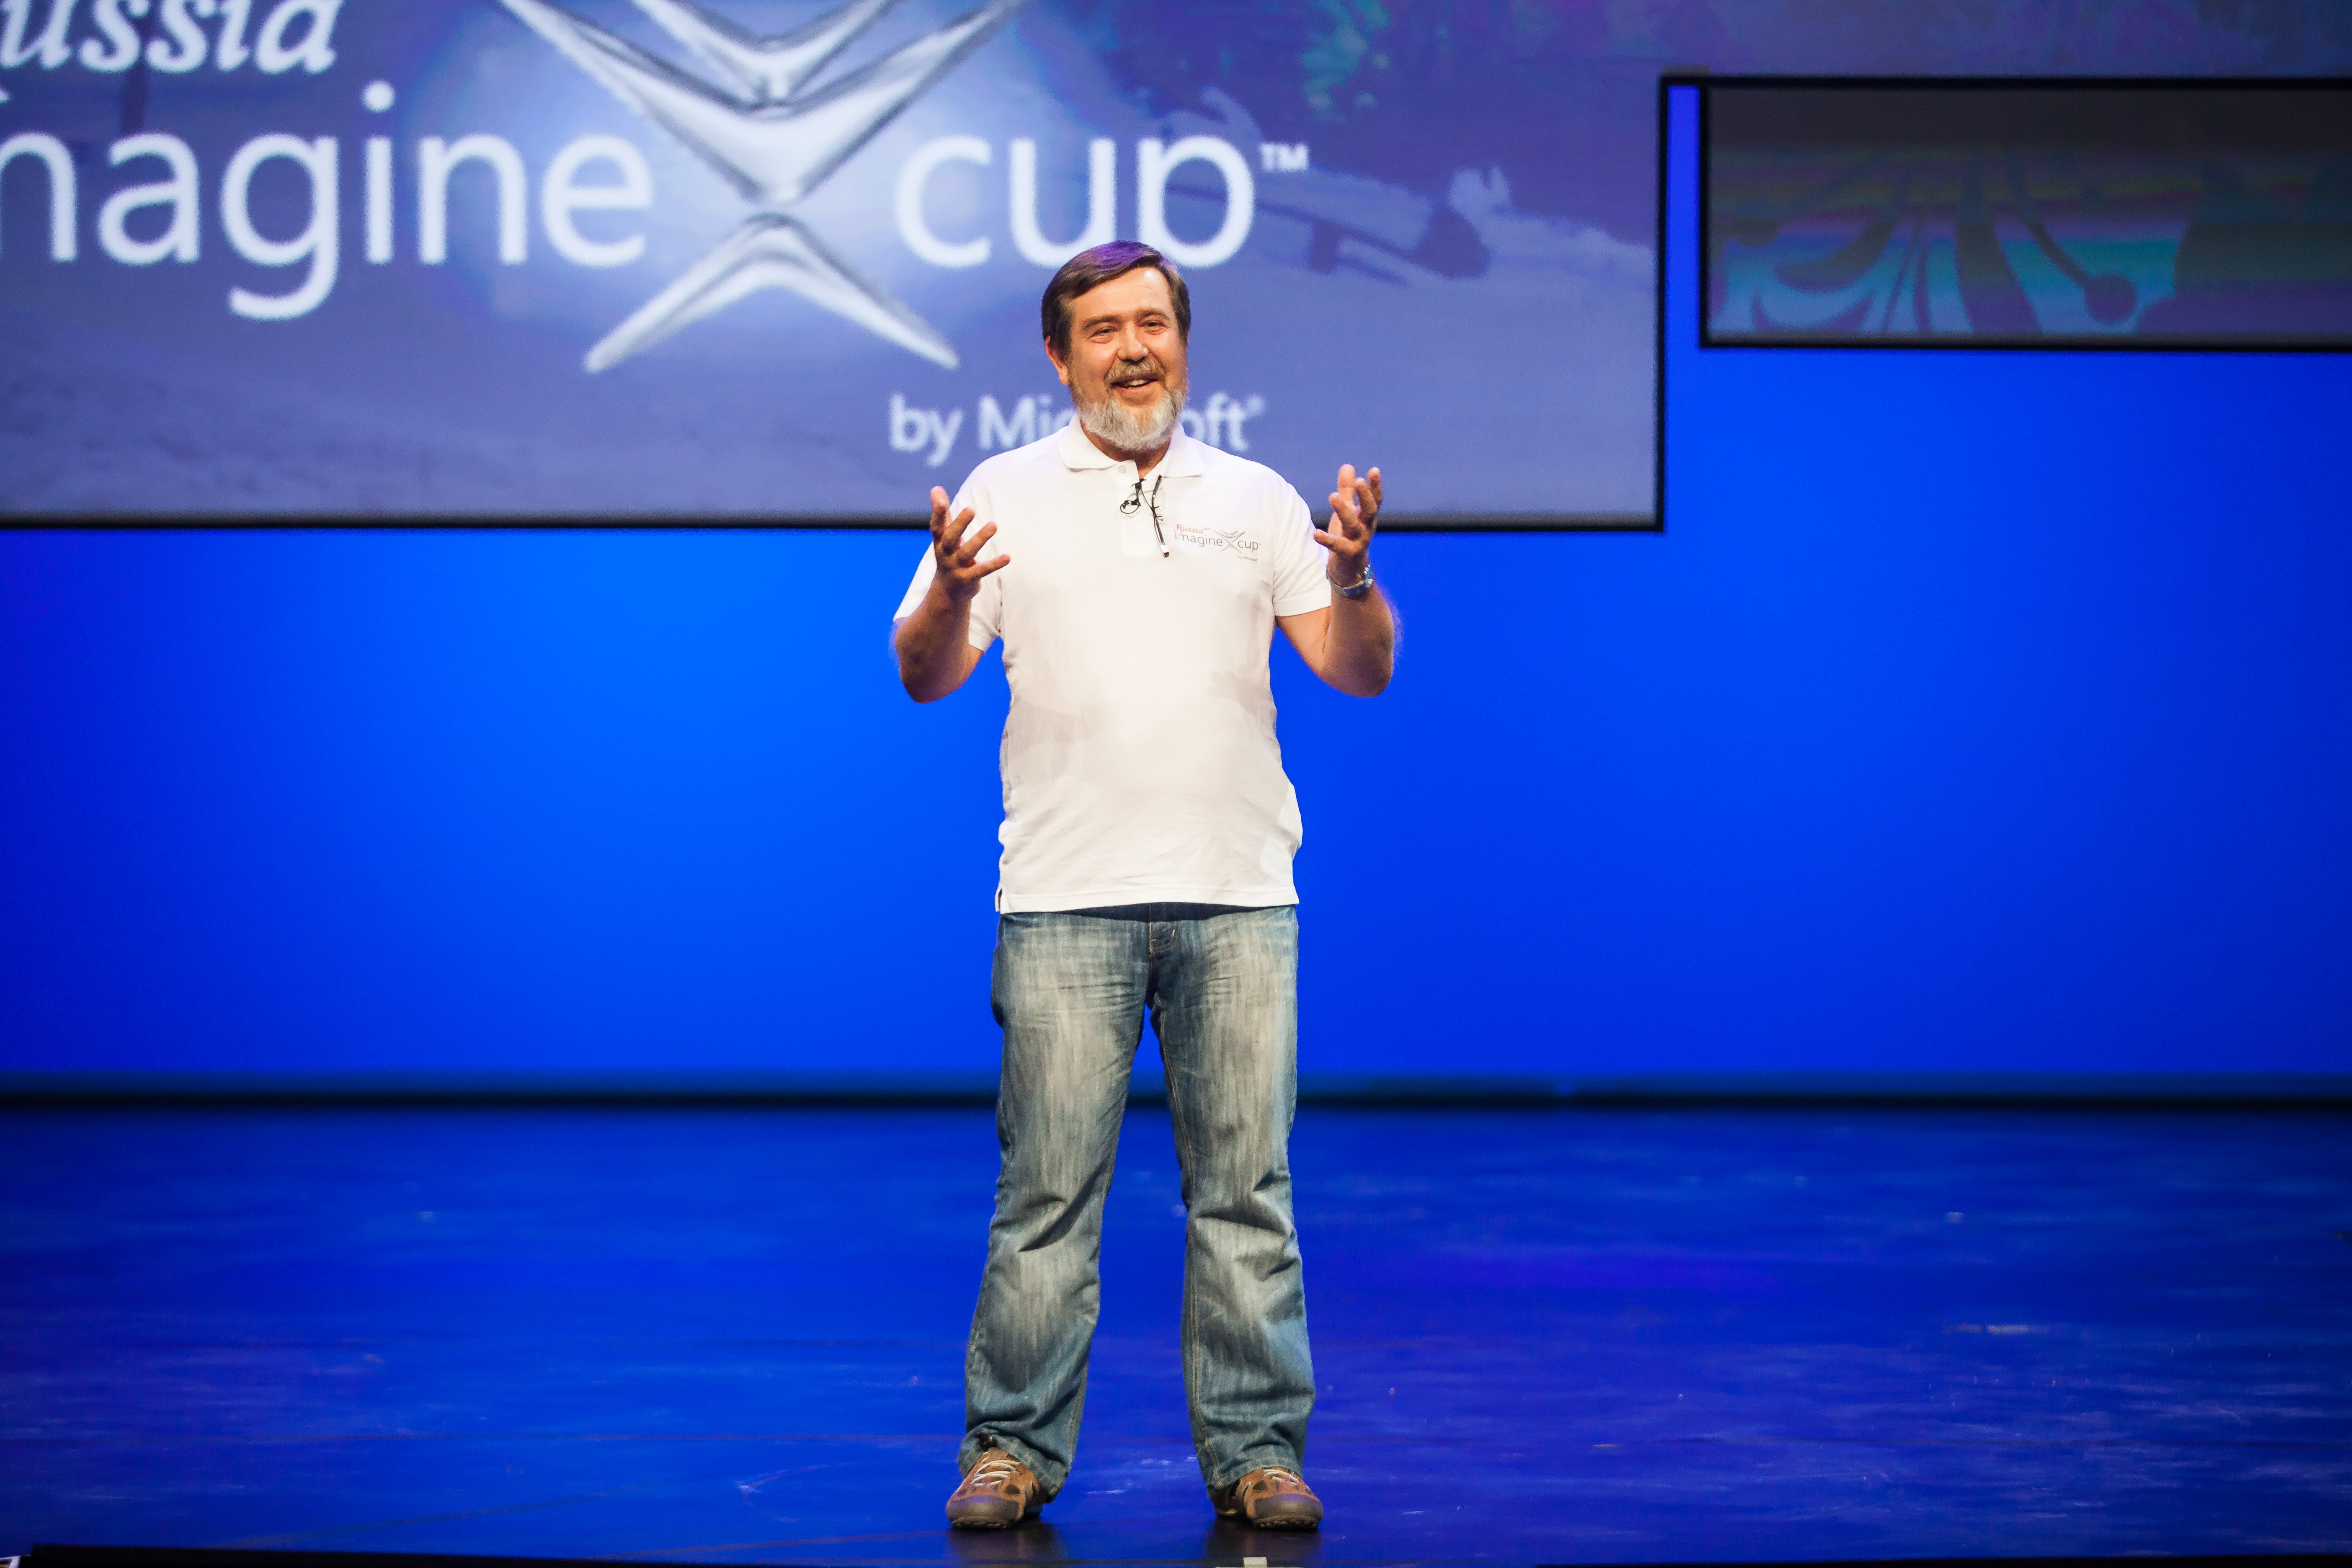
\includegraphics[width=\textwidth,height=5cm,keepaspectratio=true]{./images/Alexey_Pajitnov.jpg}}
    \caption{Alex Pajitnov, diseñador y creador de
    Tetris, en la final de la copa mundial 2013 de \textit{Image Microsoft}, en San Petesburgo, Rusia~\cite{WikipediaEN:AlexeyPajitnov}.}
    \label{fig:AlexPajitnov}
\end{figure}

Actualmente Tetris es uno de los videojuegos más vendidos de la historia con una
estimación de alrededor de 170 millones\footnote{Copias físicas y digitales.} de
copias vendidas y muchas variantes alrededor del mundo~\cite{tetris-numbers},
siendo la consola Game Boy, de la compañía Nintendo, su primer distribuidor
mayoritario~\cite{tetris-25-aniv}.

Desde el punto de vista matemático y computacional, Tetris ha planteado muchas
preguntas y planteamientos, como la posibilidad de jugar de manera infinita sin
perder\footnote{La pregunta \textit{¿sería posible jugar Tetris por siempre?}
fue enunciada en~\cite{Burgiel97howto} y la imposibilidad bosquejada.}
o las combinaciones de movimientos que posee un jugador. Tetris
ha sido objeto de estudio por diferentes campos como matemáticas, teoría de la
computación, teoría de algoritmos, psicología~\cite{Brzustowski_1992},
\cite{Burgiel97howto}, entre otros.

\section{Definición del problema}

Limitado por los gráficos de una computadora soviética llamada Electronika 60,
Pajitnov tomó la decisión de bajar la complejidad del juego de pentominó de~18
piezas, a uno de tetraminó de~7. Adicionalmente agregó lógica al juego como la
posibilidad de desaparecer líneas de piezas al ser completadas horizontalmente,
creando un juego simple y fácil de entender~\cite{tetris-history}, modificando
así el juego original.

\begin{figure}[h]
  \centering
      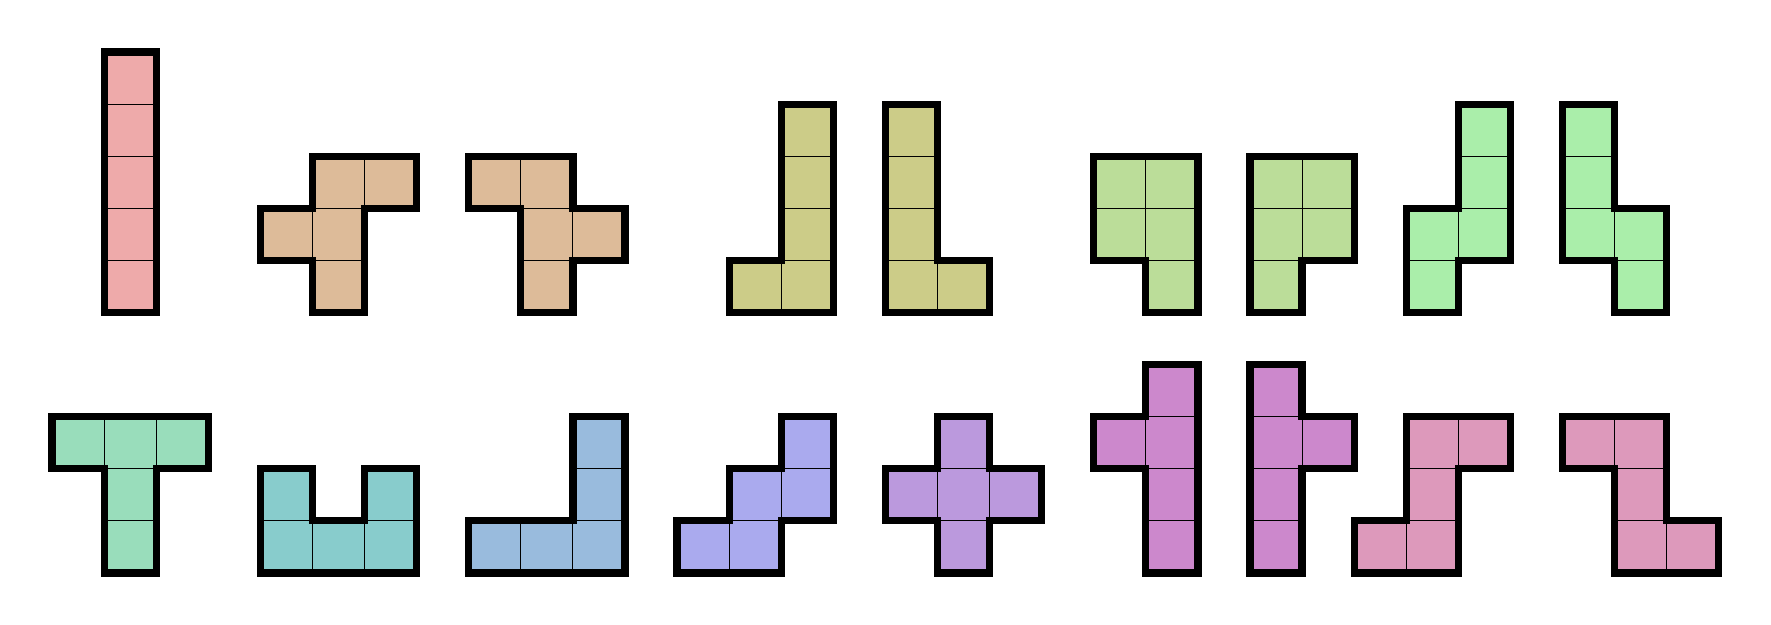
\includegraphics[width=0.8\textwidth]{./images/pentominoes}
    \caption{18 piezas del pentominó, juego original en el que se basó Alex
    Pajitnov que consiste en tratar de acomodar las 18 piezas en un
    tablero, sin dejar espacios~\cite{WikipediaEN:pentomino}.}
    \label{fig:Pentomino}
\end{figure}

La versión original del juego programada por Pajitnov hace uso de un tablero de
$10$ unidades de ancho por $20$ unidades de alto. En muchas versiones de Tetris
posteriores el tablero puede llegar a tener $n \times m$
unidades. Cuando el juego empieza, el tablero se encuentra vacío; inmediatamente
después la primera de las \textit{piezas}, que se les denomina tetraminós,
empiezan a aparecer en la parte superior del tablero.

Los tetraminós son un grupos de piezas geométricas conformada por cuatro
unidades cuadradas que se definen como \textit{celdas}. Cada celda ocupa
exactamente una unidad vacía del tablero y no pueden existir dos celdas en mismo
punto $(i \times j)$\footnote{A este punto también se puede ver como el espacio
  $(i,j)$ o la columna $j$, con la fila $i$.}. Después de aparecer en la
pantalla, las piezas bajan fila por fila, de manera pausada hasta llegar al
fondo del tablero o a un punto en el que ya no pueda bajar más debido a que se
sobrepondría a alguna otra pieza. Al ya no poder bajar más, el tetraminó
actual se mantiene en esa posición mientras un nuevo tetraminó, seleccionado
aleatoriamente dentro del grupo de siete posibles figuras (ver
\cref{fig:Tetrominos}) aparece en la parte medio superior del tablero para
ser de nuevo colocada en el tablero en alguna posición inferior.

\begin{figure}[h]
    \centering
    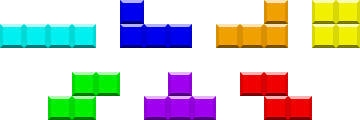
\includegraphics[width=0.6\textwidth]{./images/tetrominos}
    \caption{Los siete posibles tetrominós~\cite{WikipediaEN:tetrominos}.}
    \label{fig:Tetrominos}
\end{figure}


Los jugadores tienen a su disponibilidad la acción de rotar los tetraminós para
orientar las piezas mientras éstas caen. Otra acción que puede realizar el
jugador es mover las piezas a la columna derecha o izquierda y forzar a la 
pieza caer un nivel. Los jugadores
poseen un tiempo limitado para realizar estas acciones antes de que la pieza
sea empujada por la \textit{gravedad} simulada del juego a una fila inferior.

La mayoría de las implementaciones tienen típicamente un recuadro donde aparece
la siguiente pieza a jugar; cuando la pieza $i$ está siendo colocada en el
tablero, la pieza $(i + 1)$ es revelada en el cuadro. A ese cuadro se le llama 
\textit{cuadro de pista}~\cite{DBLP:journals/corr/cs-CC-0210020}.

Cuando toda una fila se encuentra llena de celdas de los tetrominós,
las celdas de los tetrominós en dicha fila son removidas del tablero y
las celdas de las piezas en filas superiores son desplazadas hacia niveles 
inferiores para llenar el espacio dejado por la fila removida. 
Un \textit{tetris} ocurre cuando cuatro filas son removidas al 
mismo tiempo. Si los jugadores no remueven
celdas lo suficientemente rápido, el tablero del juego se
quedará sin espacio para seguir colocando piezas y la partida
terminará~\cite{Burgiel97howto}.

Debido a los resultados obtenidos por~\cite{Burgiel97howto}, se sabe que es
imposible ganar el juego de Tetris, por lo que el objetivo principal del
jugador es maximizar la cantidad de puntos que se van acumulando durante la
partida. Estos puntos varían dependiendo de las acciones del jugador y la
interacción de las fichas en el tablero (como la desaparición de fichas o
realizar un \textit{tetris}).


\section{Un problema \textsl{NP}-completo}

En el año 2008, un equipo de computólogos publicó un artículo donde demuestran
que programar una computadora para que juegue a Tetris, es un problema \textsl{NP}-completo.
El objetivo de esta sección será enunciar, explicar los pasos y procedimientos
que la publicación~\cite{DBLP:journals/corr/cs-CC-0210020} usó, para demostrar
la \textsl{NP}-completez del juego de Tetris. El resultado de esta sección
justifica la implementación de la heurística al problema que aborda este
trabajo.

Para comenzar con la demostración, el equipo conformado por Erik D. Demaine,
Susan Hohenberger y David Liben-Nowell definieron una versión un poco diferente
al videojuego. El cambio más importante de la versión que se presenta en el artículo
es la clasificación de dos posibles flujos de información que pueden existir:
la versión que llaman \textit{offline} es aquella en la cual la entrada del programa
contiene la lista de las piezas de forma determinista, finita y ordenada que existirán
hasta un tiempo $T$. La versión \textit{online} es aquella en la que la
información de las piezas a jugar en un tiempo $T$ es sólo la pieza $P_{T}$
y, a lo más, el tetrominó $P_{T+1}$ dentro del cuadro de pista.

Aunque la demostración del problema es sobre la versión del juego
\textit{offline}, se supone en el artículo que la versión del juego \textit{online} es al menos
(hablando de complejidad computacional) tan difícil como la versión
\textit{offline}~\cite{DBLP:journals/corr/cs-CC-0210020,boumaza:hal-00926213}.
Mencionan los autores que es intuitivamente más fácil hacer jugar a la computadora con el conocimiento
total de los movimientos posteriores que debe realizar, así que la conclusión
de la \textsl{NP}-completez de la versión \textit{offline} indica la complejidad
de hacer jugar la versión \textit{online}.

Existen cuatro objetivos del juego que son demostrados, tratar de optimizarlos
es un problema \textsl{NP}-completo:

\begin{itemize}

\item Maximizar el número de filas removidas mientras se juega alguna secuencia.

\item Maximizar el número de piezas antes de que el juego se termine.

\item Maximizar el número de veces que se hace un \textit{tetris}.

\item Minimizar la altura de la columna más alta.
\end{itemize}

Para demostrar que los objetivos (y el juego) es \textsl{NP}-completo, primero
demuestran que el problema formal del juego, \texttt{TETRIS} es elemento de 
la clase \textsl{NP}; luego que la maximización
 del número de filas removidas es un problema
\textsl{NP}-duro; los demás puntos los demuestran reduciéndolos entre ellos.
La prueba inicial de la pertenencia a \textsl{NP}-duro que hacen los
autores incluye una reducción a partir del problema visto en el
\cref{sec:3-particion}.

\subsection{Formalización del juego}
\label{subsec:formalizacion}

Las reglas de Tetris son definidas rigurosamente con el fin de transparentar
la reducción y demostraciones hechas con las operaciones y propiedades del
juego. El modelo formal propuesto consiste en los siguientes
agentes y será respetado en su mayoría durante la implementación de este trabajo:

\begin{itemize}[leftmargin=0.5cm,align=left]
\item[\textbf{Tablero. }] El tablero es una red de $n$ filas por $m$ columnas
enumeradas de abajo hacia arriba y de izquierda a derecha. La casilla
$\langle i, j \rangle$ del tablero puede estar en dos estados: \textit{ocupada} o
\textit{libre}. En un tablero válido no existen filas $c$ tal que
$\langle c,k \rangle$ con $k\in \{0,1,...,m\}$ tenga
\textit{ocupadas} a todas sus casillas. Tampoco existen filas completamente vacías que se
encuentren por debajo de alguna casilla ocupada.

\item[\textbf{Piezas. }] Los ya definidos tetraminós como los mostrados en
la \cref{fig:Tetrominos}. Cada tetraminó tendrá ahora la estructura de la
forma $P = \langle t, o, \langle i,j \rangle, f \rangle$ donde cada elemento es
respectivamente:

\begin{enumerate}
        \item Un tipo de pieza. De izquierda a derecha en la  
        \cref{fig:Tetrominos}, el tipo de pieza sería:
        \texttt{I}, \texttt{RS}, \texttt{LG}, \texttt{T},
        \texttt{RG}, \texttt{LS} y \texttt{Sq}.

        \item Una orientación dada en grados: $0^{\circ}, 90^{\circ}, 180^{\circ}$ o $270^{\circ}$.

        \item Una posición $\langle m_{c},k_{c} \rangle$ donde se encuentre la casilla
        centro de la pieza.

        \item Un valor de \texttt{FIJO} o \texttt{MOVIBLE}.
\end{enumerate}

Adicionalmente, cada tipo de pieza posee un centro. Se seleccionará una
casilla y esa casilla será considerada el centro de la pieza al ser rotada.

En el estado inicial, las piezas se encuentran en una orientación $0^{\circ}$,
la posición inicial es la $\langle m ,\lfloor n/2 \rfloor \rangle$ y la pieza tiene
el valor de \texttt{MOVIBLE}.

\item[\textbf{Rotación. }] Un modelo de rotación que es una función computable
$R: \langle P, \theta, B \rangle \mapsto P'$, donde $P$ y $P'$ son orientaciones
de las piezas, $\theta \in \{-90^{\circ}, 90^{\circ}\}$ es el ángulo de
rotación y $B$ es el tablero. El artículo define las siguientes
condiciones para $R$:

\begin{enumerate}
\item Si $P = \langle t, o, \langle i,j \rangle, f\rangle$ y la rotación es válida,
entonces $P' = \langle t, (o + \theta) \mod 360^{\circ}, \langle i,j \rangle, f\rangle$
para algún $\langle i,j \rangle$. Si la rotación no es válida, entonces $P' = P$.

\item Para determinar la validez de una rotación, $R$ sólo necesita examinar
una vecindad de tamaño $O(1)$ de la pieza $P$.

\item Si todos las casillas de la vecindad de $P$ están vacías, se dice que la
rotación es válida o legal.

\item Si la rotación es legal, $P'$ no debe ocupar ninguna casilla ya ocupada
por algún otro tetrominó en $B$.

\end{enumerate}

\item[\textbf{Reglas del juego. }] La única regla para las fichas con estado
\texttt{FIJO} es que no existen movimientos válidos para ésta. Las piezas de
la forma $P = \langle t, o, \langle i,j \rangle, \texttt{MOVIBLE}\rangle$ en un
tablero $B$, tienen el siguiente conjunto de \textit{movimientos}
\footnote{Llámese ``movimiento'' a un elemento del conjunto de acciones posibles 
del jugador, en un límite de tiempo.} disponibles:

\begin{enumerate}
\item Rotación en dirección a las manecillas del reloj. $R(P, 90^{\circ}, B)$.

\item Rotación contraria a las manecillas del reloj. $R(P, -90^{\circ}, B)$.

\item Desplazamiento a la izquierda.
$P' = \langle t, o, \langle i - 1,j \rangle, \texttt{MOVIBLE}\rangle$.

\item Desplazamiento a la derecha.
$P' = \langle t, o, \langle i + 1,j \rangle, \texttt{MOVIBLE}\rangle$.

\item Deja caer. $P' = \langle t, o, \langle i,j - 1 \rangle, \texttt{MOVIBLE}\rangle$.

\item Asignar estado. Si existe al menos una casilla ocupada debajo de $P$,
entonces $P' = \langle t, o, \langle i,j \rangle, \texttt{FIJO}\rangle$.
\end{enumerate}

Para las reglas del tablero, se define una trayectoria $\sigma$ de una pieza $P$.
La trayectoria es una secuencia de movimientos válidos del estado inicial de la
pieza, hasta la asignación del estado \texttt{FIJO} de $P$. El resultado de una
trayectoria sobre el tablero $B$, es un tablero nuevo $B'$ definido con las
siguientes características:

\begin{enumerate}
\item El tablero nuevo $B'$ es inicialmente $B$ con la figura $P$.

\item Si $P$ tiene el estado de \texttt{FIJO} y para alguna fila $r$, cada
casilla de $r$ está ocupada en $B'$, las celdas
de los tetrominós en $r$ son removidos. Para cada $r' \geq r$, se reemplaza a
la fila $r'$ en $B'$ con la fila $r' + 1$ de $B'$. Múltiples filas pueden ser
removidas con una sola trayectoria.

\item Si existe alguna casilla ocupada en $B'$ donde debería estar la siguiente
pieza en su estado inicial, el jugador pierde.

\end{enumerate}

Para un juego $\langle B_{0}, P_{1}, ..., P_{p} \rangle$, una secuencia de
trayectorias $\Sigma$ es una secuencia $B_{0},\sigma_{1},B_{1},...,\sigma_{p},B_{p}$
tal que para cada $i$, la trayectoria de la pieza $P_{i}$ aplicado al tablero
$B_{i-1}$, genera el tablero $B_{i}$.

\item[\textbf{Problema formal}] Aunque el artículo contempla varios objetivos
previamente mencionados a optimizar, el problema de decisión con el objetivo
$\Phi$ del juego de Tetris, $\texttt{TETRIS}[\Phi]$, es enunciado
formalmente como sigue:

\begin{itemize}

\item \textbf{Input:} Un juego de Tetris de la forma 
$\mathcal{G} = \langle B, P_{1}, P_{2}, ..., P_{p} \rangle$.

\item \textbf{Output:} ¿Existe la secuencia de trayectorias $\Sigma$ tal que 
$\Phi(\mathcal{G}, \Sigma)$ no resulte en una partida perdida?

\end{itemize}

\end{itemize}

Una vez definido minuciosamente el modelo formal de Tetris, incluyendo las
reglas y los objetos que participan en una partida, se procede a discutir su
complejidad.

\subsection{La clasificación de \texttt{TETRIS}}

Se sabe por las definiciones del \cref{sec:np-def}, que para que
\texttt{TETRIS} esté en \textsl{NP}-completo, debe cumplir con que
\texttt{TETRIS} $\in$ \textsl{NP}-duro y $\texttt{TETRIS} \in \textsl{NP}$.

Para llegar a la conclusión de la \textsl{NP}-completez, los autores tuvieron
que proponer y demostrar ciertos lemas y teoremas enunciados a continuación:

\begin{itemize}[leftmargin=0.5cm,align=left]

\item[\textbf{Teorema 2.1}] Para cada objetivo \textit{acíclico}\footnote{Se dice que una
función objetivo $\Phi$ es acíclica si para todo juego $\mathcal{G}$ en los que 
exista una trayectoria $\Sigma$ tal que $\Phi(\mathcal{G},\Sigma)$ no
pierde, entonces existe una trayectoria $\Sigma'$ tal que
$\Phi(\mathcal{G},\Sigma')$ no pierde y no existen estados repetidos de
las piezas en $\Sigma'$.} comprobable $\Phi$, se tiene
que \texttt{TETRIS}[$\Phi$] $\in$ \textsl{NP}.

En el artículo se da un algoritmo \textsl{NP} para \texttt{TETRIS}[$\Phi$]. Los autores
argumentan que dado una $\Sigma$ aleatoria, se puede verificar que
$\Phi(\mathcal{G}, \Sigma)$, en tiempo polinomial\footnote{Se nombrará de
manera genérica a la función de verificación en tiempo polinomial, función
\texttt{POLY}.}  ya que también se puede verificar
$\texttt{POLY}(|\mathcal{G}|, |\Sigma|) = \texttt{POLY}(|\mathcal{G}|)$
debido a que cada de las $p$ trayectorias en $\Sigma$ contiene a lo más
$4 \cdot |B| + 1$ estados a verificar, $|B| = n\times m$ con $n$ y $m$ el número de filas
y columnas de cada tablero.

\item[\textbf{Lema 2.2}] El objetivo \textit{k-filas-removidas}\footnote{
$\texttt{k-filas-removidas}:\mathcal{G} \times \Sigma \rightarrow \mathds{N}$
nos regresa el número de filas removidas durante un juego de Tetris.} es
\texttt{POLY} verificable y acíclico.

La corta demostración de este lema se realiza mediante la argumentación
de que \texttt{k-filas-removidas} es acíclico porque sólo depende del estado
de cada pieza que es colocada al final de cada trayectoria en el tablero.
Es \texttt{POLY} verificable ya que sólo es necesario recorrer cada tablero que
regrese cada trayectoria en a lo más $O(m \cdot n \cdot |\Sigma|)$.

\item[\textbf{Teorema 3.1}] \texttt{3-PARTITION} es un problema \textsl{NP}-completo.

Este teorema es discutido en la \cref{sec:3-particion} y demostrado
en~\cite{Garey:1990:CIG:574848}.

\item[\textbf{Teorema 3.2}] El juego $\mathcal{G}(\mathcal{P})$ es polinomial
respecto a $\mathcal{P}$.

Para explicar este teorema, primero hay que explicar la decisión que tomaron
Demaine,  Hohenberger y Liben-Nowell en su artículo para el problema de reducción:

Los autores decidieron crear la reducción del problema \texttt{3-PARTITION}
debido a su propiedad de ser fuertemente \textsl{NP}-completo; esto incluye
valores de entrada $a_{i}$ y $T$ unitarios. También de enfocan en instancias
específicas de \texttt{3-PARTITION}:

\begin{enumerate}
\item Para cada conjunto $S \subseteq \{a_{1},...,a_{3s}\}$, si $\sum_{a_{i} \in S} a_{i} = T$
entonces $|S| = 3$.

\item $T$ es par.

\item Si $\sum_{a_{i} \in A_{j}} a_{i} \neq T$ entonces
$\left|T - \sum_{a_{i} \in A_{j}} a_{i} \right| \geq 3s$.
\end{enumerate}

Dada una instancia $\mathcal{P} = \langle a_{1}, ..., a_{3s},T \rangle$ que
cumpla las tres condiciones de arriba, $\mathcal{G}(\mathcal{P})$ es un juego
de Tetris que elimina a todas las piezas si $\mathcal{P}$
tiene como respuesta un valor booleano de \texttt{TRUE}.

El tamaño del tablero y el número de piezas dependerá de los valores $S$ y
$T$ del problema de la \texttt{3-PARTITION}: el tamaño del tablero resultante
de $\mathcal{G}(\mathcal{P})$ es de $6T + 22 + 3s +  O(1)$ filas por $6s + 3$
columnas, mientras que el número de piezas totales del juego será de:

\begin{displaymath}
\sum\limits_{i=1}^{3s}[3 + 5a_{i} +2] + s + 1 + \left( \frac{3T}{2} + 5 \right)
= 16s + 5sT + \frac{3T}{2} + 6.
\end{displaymath}

Los valores $a_{i}$ y $T$ están representados como valores unarios (por la
naturaleza del sistema de conteo de casillas en el tablero) por lo que
se puede suponer siempre una transformación polinomial a la hora de construir
el juego conforme a la opinión de los autores de la demostración.

\item[\textbf{Teorema 4.1} (Completez)]  Para cada instancia
$\mathcal{P}$ que tenga como respuesta un valor booleano de \texttt{TRUE} del
problema de la \texttt{3-PARTITION}, existe una secuencia de trayectorias
$\Sigma$ que \textit{limpie}\footnote{En este contexto, limpiar el tablero
tiene el significado de mantener el juego sin piezas, es decir, que todas
las piezas jugadas sean en algún punto removidas del tablero.}
el tablero $\mathcal{G}(\mathcal{P})$ sin que el juego termine, o el jugador
pierda. \\% \linebreak

 \begin{figure}[h!]
\centering
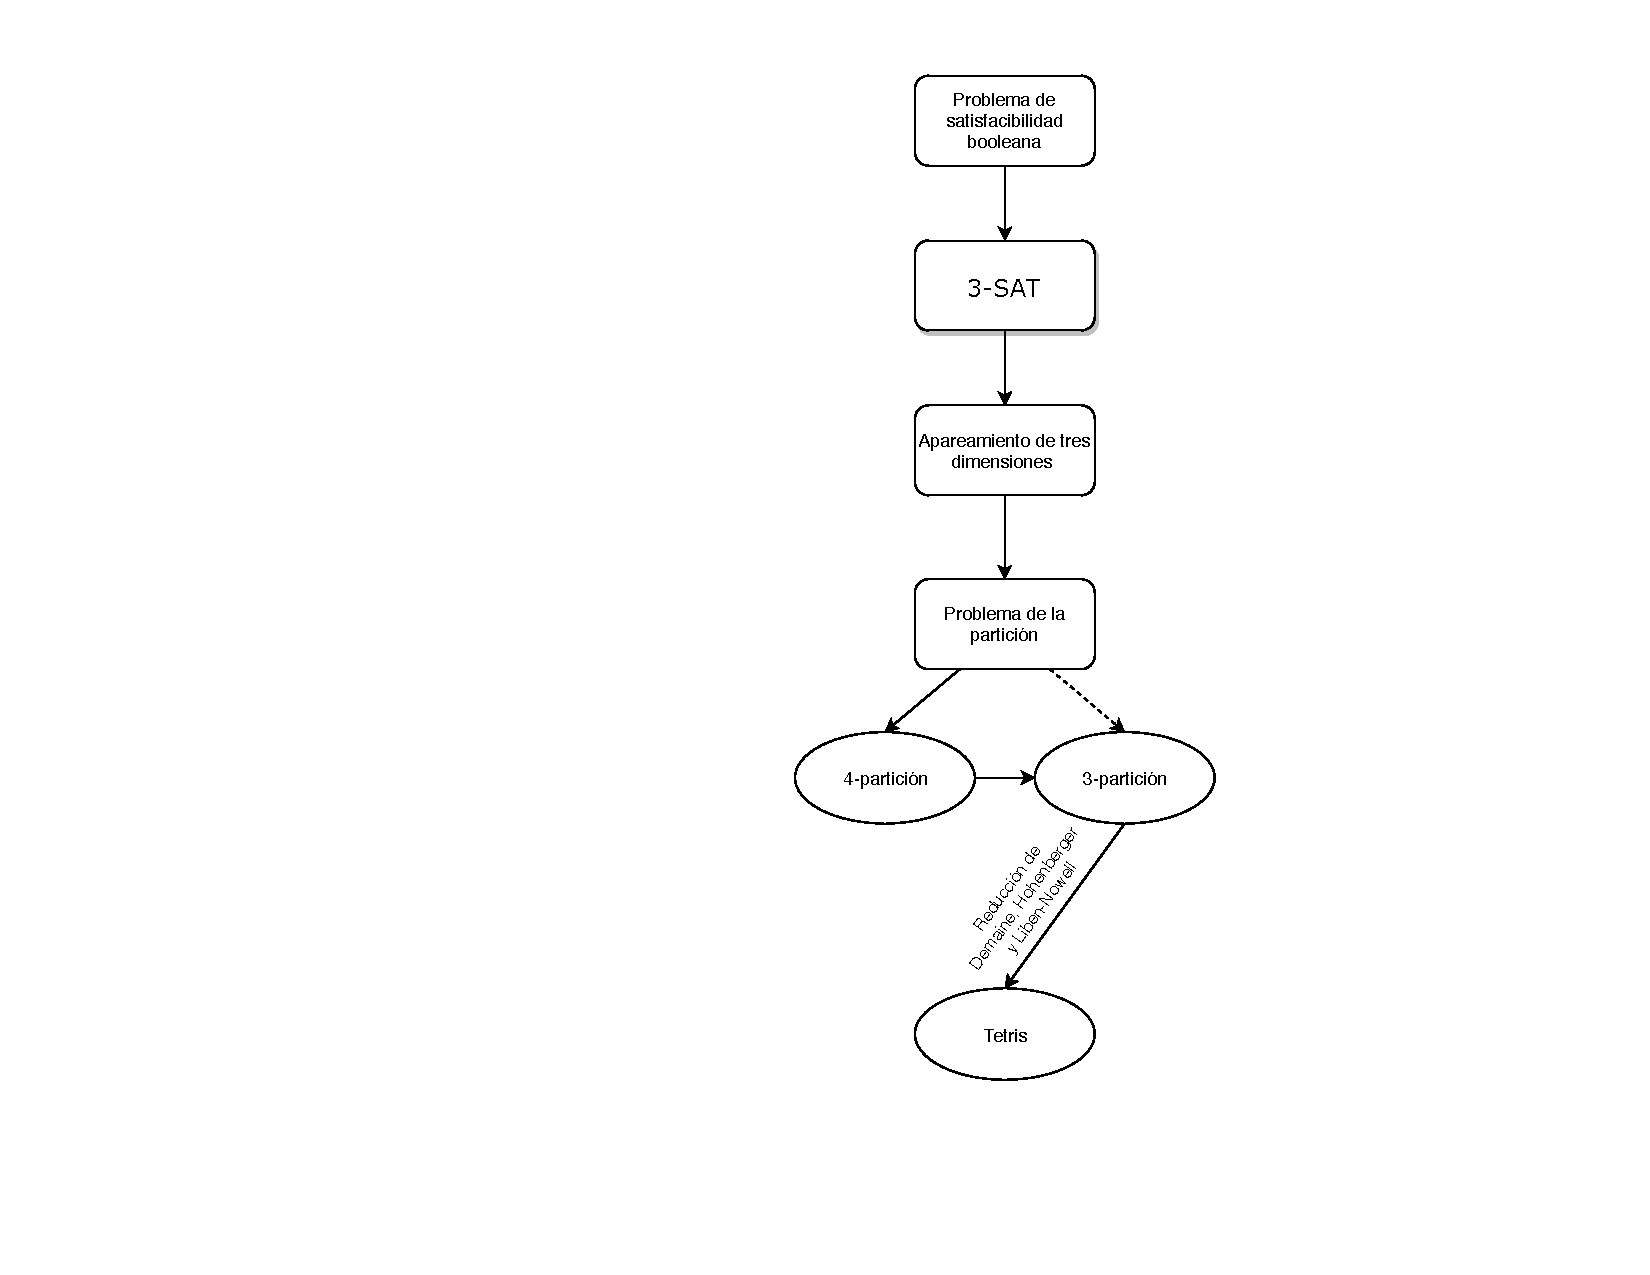
\includegraphics[width=0.4\textwidth,keepaspectratio,trim={12cm 6cm 7cm 1cm}]{./images/4_3_1.pdf}
\linebreak\linebreak\linebreak\linebreak\linebreak\linebreak
\caption{Extensión del diagrama de la \cref{fig:secuenciaNP} de las reducciones
polinomiales desde \texttt{SAT} hasta Tetris con $\mathcal{G}(\mathcal{P})$.}
\end{figure}

La forma que proceden en esta demostración es partiendo por la condición de
veracidad de \texttt{3-PARTITION}; aprovechan la partición
de los conjuntos $A_{i}$ para asociar a los tetrominós con algún número,
 acomodarlos en algo que los autores llaman \textit{cubetas}, que son
 divisiones del tablero que se le asigna a cada $A_{i}$ y así, asegurar no dejar
 espacios casillas sin llenar. De manera bastante ilustrativa construyen estas
 secuencia de piezas o configuraciones donde se aseguran no existan huecos en las filas,
 produciendo así su \textit{limpieza} y remoción del tablero.

Dada la reducción propuesta
$\texttt{3-PARTITION} \leq_{\mathcal{G}(\mathcal{P})} \texttt{TETRIS}$,
 la demostración dentro del artículo y las definiciones de
 \cite{arora2009computational} en la \cref{sec:np-def}, se puede afirmar que
 \texttt{TETRIS} $ \in $ \textsl{NP}-duro.

\item[\textbf{Lema 5.10}] El modelo de rotación propuesto es suficiente.

Cubriendo todos los posibles casos con los siete tetraminós, los autores
muestran que no existe combinación de rotaciones en el que las piezas
puedan (o piezas diferentes a ellas no puedan) llenar ciertos espacios del
tablero.

\item[\textbf{Teorema 5.16}] Si existe una estrategia válida para
$\mathcal{G}(\mathcal{P})$, entonces $\mathcal{P}$ es una instancia de
\texttt{3-PARTITION} que tiene respuesta un valor booleano de \texttt{TRUE}.

El artículo, va un poco más allá y plantea, discute y demuestra la propiedad
de que la robustez o exactitud\footnote{Viene del inglés \textit{soundness}.},
que significa que cualquier solución encontrada sea correcta.

Inmediatamente después de esta última demostración, el artículo enuncia como
consecuencia a todos los teoremas y lemas enunciados arriba, el siguiente
teorema:

\item[\textbf{Teorema 5.17}] \texttt{TETRIS}[\textit{k-filas-removidas}] es \textsl{NP}-completo.

Habría que recordar la definición que se enunció en el \cref{sec:np-def}; dice
que para que un problema esté dentro de la clase \textsl{NP}-completo, debe cumplir
que esté tanto en \textsl{NP} y en \textsl{NP}-duro. Estas propiedades se demuestran
en el \textbf{Teorema 3.1}. La parte de pertenencia a \textsl{NP}-duro se construye
por el \textbf{Teorema 4.1}, usando la reducción, los teoremas 2.1, 3.1, 3.2 y
5.16 y los lemas 2.2 y 2.10 se concluye que
\texttt{TETRIS}[\textit{k-filas-removidas}] $\in$ \textsl{NP}-completo.

\end{itemize}

Si bien, el artículo no termina con este teorema y va más allá, demostrando la
complejidad de cada uno de los objetivos a optimizar, para propósitos de este
trabajo, es suficiente este resultado por lo que en los capítulos posteriores
se habla de herramientas técnicas y la implementación del problema.

%%% Local Variables:
%%% mode: latex
%%% TeX-master: "../main"
%%% End:


\chapter{Tecnologías utilizadas}

Aunque el concepto de complejidad de un algoritmo, clases de complejidad y
eficiencia mantienen un estado invariante al entorno de desarrollo de
los programas, el análisis de la experimentación está inevitablemente
comprometido por el desempeño del hardware y software que se usa. Para
darle sentido a los resultados, es muy importante conocer las herramientas 
usadas, así como el ambiente en el que los experimentos fueron realizados.

\section{Python}

En la década de los ochenta, en el centro Wiskunde de informática, en Ámsterdam,
Guido van Rossum trabajaba como desarrollador de un lenguaje de programación
llamado \textit{ABC} cuyo propósito era ser una herramienta de desarrollo
fácil de aprender para personas no acostumbradas a programar. Rossum vio la
necesidad de crear un lenguaje de \textit{scripting}\footnote{En
algunos textos referidos como \textit{Guiones del intérprete de comandos}, son
programas en las que sus órdenes son ejecutadas de manera
secuencial~\cite{interprete-comandos}.} sobre su proyecto en el lenguaje ABC,
por lo que creó una máquina virtual, un programa \emph{parser} y otro de ejecución de
comandos; agregó una sintaxis básica, usó indentación para definir bloques
y creó un pequeño conjunto de tipos de datos. Así nació
Python~\cite{python-interview}.

Python es un lenguaje de programación de propósito general, Turing completo,
dinámicamente tipificado y con influencia de múltiples paradigmas; incluidos
pero no limitado a orientación a objetos, funcional e imperativo~\cite{python}.
Una de las principales características por las que Python es reconocido, es por
su manera de definir bloques de código: la indentación de un programa en Python
es fundamental para la semántica de un programa.

Python se encuentra desde el 2003 como uno de los lenguajes de programación
más populares de acuerdo al índice de clasificación de la comunidad programadora
TIOBE~\cite{tiobe}. Cientos de compañías como Google, Yahoo, Disney Animation,
NASA, IBM, usan Python como lenguaje de desarrollo para resolver
problemas en diversas áreas~\cite{python-usage}.

Actualmente existen muchas versiones de Python; las más usadas son 
las versiones 2.7 y 3.5 que en conjunto con el administrador de
paquetes\footnote{Un administrador de paquetes es un programa que tiene como
propósito la instalación, actualización y configuración de paquetes de software.}
PIP, proveen de cientos de bibliotecas listas para usar e implementar soluciones
a problemáticas de diversa índole~\cite{python}.

Otra de las ventajas más grande que posee Python sobre otros lenguajes de alto
nivel, es su ambiente de desarrollo
y ejecución; Python posee como herramienta la creación de sus propios ambientes
virtuales con sus propio sistema de archivos aislados e independientes al
sistema local. La ventaja principal de mantener un ambiente de desarrollo
independiente, es la instalación y manejos de paquetes en un sistema donde
aquellos que poseen otros ambientes virtuales o el mismo ambiente
local no interfiera ni genere conflictos por paquetes previamente instalados o
por versiones diferentes~\cite{venv}. %python3 -m venv ./.env

En los últimos años Python en su desarrollo se ha orientado a mejorar la
eficiencia de tiempo de respuesta de sus llamadas a sistema; la forma en la que
Python mejora su velocidad aún siendo un lenguaje que típicamente usa un
intérprete, es generando archivos con extensión \texttt{.pyc}, que son archivos
en lenguaje máquina, los cuales contienen funciones e instrucciones previamente
ejecutadas y optimizadas para su posterior uso repetitivo~\cite{python}. De
cualquier manera, Python sigue teniendo algunos problemas para escalar a
sistemas grandes y complejos.


\subsection{pygame}

Una de las razones por las que Python se hizo altamente reconocido, fue por la
facilidad de hacer uso de bibliotecas externas al núcleo del lenguaje. Existen
una gran cantidad de bibliotecas muy conocidas y usadas mundialmente,
ya sea por la facilidad que proveen o por lo conveniente que resultan sus
soluciones. Un ejemplo es la
biblioteca Numpy que posee un conjunto de funciones de uso científico ampliamente
reconocido por la comunidad investigadora, por ser de gran utilidad en numerosos 
proyectos~\cite{numpy}.

La biblioteca pygame es una biblioteca de Python, de código abierto que sirve para realizar 
aplicaciones multimedia como animaciones o videojuegos; existen 
alternativas ya programadas que tiene como propósito ejecutar videojuegos 
publicados originalmente para la consola \textit{Nintendo Entertainment System} 
o \textit{NES}, sin embargo, las opciones consideradas presentan la inconveniencia de no poder 
modificar el tablero a voluntad de manera directa y simplificada.~\cite{gym-tetris,nespy}.

Si bien el propósito de las bibliotecas pygame puede ser la creación de 
videojuegos donde la optimización de gráficos y ejecución requiere el mayor 
cuidado, sólo se usará como una herramienta de visualización de resultados debido 
a la naturaleza de la heurística de colonia de abejas artificiales~\cite{pygame}.



\section{Git}

Durante el desarrollo de cualquier proyecto de software existen muchas herramientas útiles para
mejorar y hacer más eficiente el flujo de trabajo. Un ejemplo de software útil son
los controladores de versiones, también llamados \textit{versionadores}.
Los controladores de versiones son sistemas que
mantienen un registro (en un lugar llamado repositorio) de todos los cambios
realizados a un conjunto de archivos rastreables, produciendo la oportunidad de
observar un historial de modificaciones realizadas en un periodo de
tiempo~\cite{git-about}. Existen dos categorías principales de controlador de
versiones: los versionadores de repositorios centralizados que son aquellos en los que los
archivos que están siendo rastreados se encuentran en un repositorio central,
único, que todos los desarrolladores modifican; y los versionadores de repositorios
distribuidos que mantienen muchas copias del código en distintas computadoras e
implementan un sistema de comunicación de cambios mediante un historial. De este
último tipo es uno de los versionadores más usados: Git~\cite{scopatz2015effective}.

Git fue desarrollado en el 2005 por el mismo creador de uno de los proyectos más
grandes de software libre que existe; el proyecto Linux necesitaba de un controlador de
versiones debido a su particularidad de ser un sistema operativo que es
modificado por miles de personas alrededor del mundo. Linus Torvalds
consideró necesario la creación de Git como herramienta rápida, segura y que
soportara desarrollo de código de manera no lineal, para mantener una buena
comunicación de desarrollo del proyecto Linux~\cite{git-about2,git-commit}.

Si bien el uso básico de Git es sencillo, dominarlo puede llegar a ser un
trabajo de años de experiencia. Un programador sin experiencia en la herramienta
puede comenzar a realizar seguimiento y registro de cambios en el sistema de
archivos con un par de comandos (\texttt{git init}, \texttt{git add -A},
\texttt{git commit} en particular).

Los cambios son guardados dentro de un árbol de registros donde cada rama 
del árbol pertenecerá a una secuencia de historias. 
Cada cambio agregado y almacenado genera una huella digital única llamada \textit{hash}. 
Este \emph{hash} único es el identificador del espacio
temporal del historial donde se almacena la información $I$ en el tiempo $T$~\cite{git-about}.

Una de las conveniencias de usar Git como herramienta para proyectos de desarrollo 
de software es poder regresar a algún punto en una versión del historial. Es
conveniente conocer el \emph{hash} con el comando \texttt{git log} y familiarizarse con 
la orden \texttt{git revert}.

Es importante aclarar que el uso de Git va más allá de mantener un registro 
y poder mover el estado actual del proyecto por uno de sus estados 
almacenados; Git posee características que benefician al trabajo en equipo,
depuración de errores, pruebas y mantenimiento, desarrollo remoto y varias
características que lo han hecho uno de los programas con mayor número de usuarios y 
de traducciones: Git existe en doce idiomas y más de seis traducciones parciales.

Durante el desarrollo de este proyecto se usará Git de manera constante
para llevar un registro de todos los cambios hechos en el código de la
implementación de la heurística.

\section{Ambiente físico}
\label{sec:ambiente-fisico}

Invariablemente los resultados obtenidos pueden ser muy diferentes dependiendo 
el equipo en el que se prueben así como su sistema operativo y su versión correspondiente. 
El hardware es mejorado con notoriedad cada poco tiempo de acuerdo a las observaciones 
como las de Mark Kryder o la reconocida ley de Moore, por lo que no es de extrañarse 
que con el paso de tiempo los resultados parecieran mejorar. El software también 
sufre de mejoras; algoritmos de funciones de los sistemas operativos son actualizados 
constantemente para garantizar el mayor rendimiento posible. 

El desarrollo, pruebas y análisis fueron realizadas en una computadora 
ASUS, ZenBook Pro 14 modelo UX450FDX. La velocidad de comunicación de 
la memoria RAM, 8 GB DDR4 Synchronous es de 2,400 MHz (a 0.4 ns). Los 
tres niveles de cache (L1, L2 y L3) poseen respectivamente 256 KB, 1 MB y 6 MB.
El procesador del ambiente de ejecución es de la marca Intel(R) Core(TM), 
modelo i5-8265U, x86\_64, 8 núcleos de dos hilos cada uno y corre a una velocidad 
promedio máxima de 3.9 GHz. 

El sistema operativo instalado en la computadora es una distribución de GNU/Linux 
Debian, con una versión actualizada del kernel 4.19.0-0.bpo.4-amd64, que corre 
sobre la versión de la arquitectura de 64 bits. La versión del lenguaje de programación usada 
también es relevante debido a que los lenguajes de programación son constantemente 
modificados y mejorados. El ambiente de desarrollo que se usa es la versión 
de Python 3.5.3.

%%% Local Variables:
%%% mode: latex
%%% TeX-master: "../main"
%%% End:


\chapter{Análisis y diseño de la implementación}

Un buen diseño de software 
apegado a buenas prácticas de programación contribuyen a la obtención 
de resultados de calidad, menos errores durante la implementación y un 
entendimiento más sencillo para terceros. Durante este capítulo, se analizan  
las decisiones de la implementación y el motivo del diseño. Todas las clases y 
funciones discutidas a continuación se encuentran en el 
\cref{apendice:code} y en la liga 
\url{https://github.com/ricardorodab/abc-tetris}.

\section{Análisis del sistema}

Para encontrar soluciones a la colocación de las piezas de Tetris, primero se tiene que 
partir del poder acceder a toda la información del juego para el análisis de los desenlaces. 
En el \cref{subsec:formalizacion} se realiza la formalización del juego y con ella las 
reglas a seguir durante la implementación:

\begin{enumerate}
\item Se debe diseñar un tablero que almacene la información del conjunto de 
piezas.

\item Se debe tener piezas que posean un tipo específico, posición y orientación. 

\item Se debe programar un modelo de rotación específico para las piezas de 
acuerdo a su tipo.

\item El tablero, piezas y modelo de rotación deben estar regidos en todo 
momento por las reglas del juego.
\end{enumerate} 

El objeto que contenga los entes principales del juego, deben también tener 
métodos de obtención de información relevantes a la heurística como datos que 
sirvan para generar una función de costo y métodos para forzar ciertos 
comportamientos indicados por un objeto externo (como lo es la misma heurística 
en este caso) para pasar de un estado del juego a un estado siguiente.

Una regla adicional necesaria para la utilización de cualquier conjunto de reglas 
a optimizar es que todo objeto que reciba la heurística debe ser ``clonable'', 
esto quiere decir que exista un método o función la cual regrese un objeto idéntico 
al que lo llama y que la heurística tenga la libertad de modificar sin afectar el 
estado del objeto clonado original.

Del lado de la heurística el elemento más importante a considerar es el 
comportamiento de la colmena como un conjunto de funciones que realizan 
las abejas que habitan en ella en un periodo de tiempo. Cada abeja 
creada dentro de la colmena tiene la tarea de explorar y trabajar o 
de observar. La necesidad de dividir a las abejas de esta manera se puede entender 
en el artículo \cite{karaboga2008performance} donde el autor de la heurística, 
Karaboga, realiza pruebas que concluyen en que tener el 50\% de abejas observadoras 
incrementa el néctar de sus soluciones. 

Durante una iteración de la colmena se deben realizar las siguientes acciones: 

\begin{enumerate}
\item Si la colmena no tiene abejas, inicializarlas.

\item Mandar a llamar al método que libera a las exploradoras y las transforma en 
trabajadoras asociadas a una fuente.

\item Mandar a llamar a las abejas trabajadoras para que recolecten néctar de su 
fuente y generen información para hacer el \textit{waggle-dance}.

\item Hacer que las abejas observadoras escojan una fuente y ejecutar las 
funciones implementadas para la observación de cada fuente vecina. 
 
\end{enumerate}

El problema específico a resolver no debe afectar el comportamiento de la 
heurística por lo que se puede aprovechar las propiedades de lenguajes en el 
paradigma funcional que ofrece 
Python y asignar funciones como parámetros y atributos para que la ejecución de las abejas 
sea independiente al problema y sean los atributos de cada abeja los 
llamados para evaluar las fuentes.

Un último paso para poder operar con la heurística y el juego es el conjunto 
de métodos que realizan la comunicación entre ambos; los resultados se deben unir de alguna 
manera ya que el resultado de cada iteración es la entrada de la 
siguiente. Las funciones que las abejas esperan y necesitan para realizar su 
trabajo dentro de la heurística también es necesario comunicarlo a la hora 
de instanciar la colmena.

Una buena práctica es que los parámetros de experimentación no sean modificados 
directamente en el código sino que se deben encontrar como entrada, en algún archivo 
de configuración para su fácil modificación y preservar así un buen diseño. Es 
conveniente implementar métodos asociados al manejo del archivo de entrada así como un objeto 
que contenga siempre estos parámetros desde el principio de la ejecución del programa.

\subsection{Abejas observadoras}

Las abejas observadoras tienen un nivel de dificultad un poco mayor de diseño e 
implementación debido a la naturaleza de las acciones que toman. Una abeja 
observadora primero le es asignada una fuente $i$ de las ya trabajadas con 
probabilidad 

\begin{displaymath}
  P_{i} = \frac{F(\theta_{i})}{\sum_{k=1}^{n} F(\theta_{k})}.
\end{displaymath}

Se debe considerar el caso donde después de recorrer todas las fuentes, la 
abeja observadora se queda sin alguna asignación de fuente. 
Una abeja observadora no se debe quedar 
sin fuente por lo que de existir un abeja en este caso se debe volver a iterar 
sobre todas las fuentes hasta que le sea asignada. Una solución para evitar este 
problema del no determinismo a la hora de asignar parejas, es duplicar la 
probabilidad de asignación de todas las soluciones por cada iteración para 
evitar que se recorra demasiada veces la lista de fuentes. 

Un problema aún mayor es la localización de fuentes vecinas. En el caso particular 
de Tetris, se necesita alguna manera de conseguir una fuente vecina a un punto 
del tablero. La definición de fuente vecina es 

\begin{displaymath}
  \theta_{i}(c+1) = \theta_{i}(c) \pm \phi_{i}(c)
\end{displaymath}

\noindent
donde $\theta_{i}(c)$ es la solución $i$-ésima. El primer enfoque resolutivo de este 
problema fue el jugar movimientos aleatorios posteriores a una fuente, 
sin embargo dichos movimientos serían correspondientes a un punto futuro de la partida 
por lo que no se considera una fuente vecina sino la fuente $i$ explotada como 
lo haría una abeja trabajadora. 
Una forma en la que $\phi_{i}(c)$ es encontrada es mantener un registro de 
movimientos que se jugaron para llegar a $\theta_{i}(c)$ y poder cambiar algunos 
movimientos previos con ayuda de un \textit{historial}.

El historial no es más que una lista de movimientos $L_{\theta}$ que se han hecho hasta un 
tiempo $T$. Es posible eliminar un número aleatorio $\delta_{1}$ de movimientos 
para posteriormente agregar en la lista otro número de movimientos aleatorios $\delta_{2}$ hasta 
llegar a $T$ con una lista de movimientos $L_{\phi}$. Los tiempos $T$ fueron seleccionados 
como los puntos en 
el que las piezas son fijadas, esto debido a que ese comportamiento es una invariante 
para todas las piezas del juego.

\begin{tikzpicture}[
    node distance = 21mm and 7mm,
    box/.style = {draw, minimum size=8mm, inner sep=0pt, outer sep=0pt, anchor=center},
      pin edge = {Straight Barb-, shorten <=1mm,semithick}]
        \node (h2) [box] {Izq};
		\node (h1) [box, left=of h2] {Der};
		\node (h3) [box, right=of h2]    {Gir};
		\node (h4) [box, right=of h3]    {Cae};
		\node (q_dots) [draw=none, right=of h4] {$\cdots$};
		\node (hk) [box, right=of q_dots] {$Mov_{m}$};
		
		\node (h5) [box, below=of h4] {Izq};
		\node (h32) [draw=none, left=of h5] {};
		\node (q_dots_two) [draw=none, right=of h5] {$\cdots$};
		\node (hl) [box, below=of hk] {$Mov_{n}$};
		
		
		\draw[dashed,-Straight Barb, shorten <=1mm, shorten >=1mm]
    (h3.south) edge [bend right]   (h5.north);	
		
		\draw[-Straight Barb, transform canvas={yshift= 0mm}]
    		(h1) edge   (h2);
    	\draw[-Straight Barb, transform canvas={yshift= 0mm}]
    		(h2) edge   (h3);
    	\draw[-Straight Barb, transform canvas={yshift= 0mm}]
    		(h3) edge   (h4);
    	\draw[-Straight Barb, transform canvas={yshift= 0mm}]
    		(h4) edge   (q_dots);    		
    	\draw[-Straight Barb, transform canvas={yshift= 0mm}]
    		(h5) edge   (q_dots_two);
    	\draw[-Straight Barb, transform canvas={yshift= 0mm}]
    		(q_dots_two) edge   (hl);
    	\draw[-Straight Barb, transform canvas={yshift= 0mm}]
    		(q_dots) edge   (hk);
    	\draw [decorate,decoration={brace,amplitude=6pt,raise=5ex}]
  (h1) -- (hk) node[midway,yshift=4em]{$\theta_{i}$};
  
 		 \draw [decorate,decoration={brace,amplitude=7pt,mirror,raise=5ex}]
  (h32) -- (hl) node[midway,yshift=-4em]{$\phi_{i}$};
    \end{tikzpicture}


\subsection{Función de costo}

La función de costo o también conocida como función \textit{fitness} es la encargada 
de calificar una solución propuesta por la colmena para su posterior uso. 
Si una función de costo es de baja calidad, los resultados serán de igual forma 
de baja calidad. Una buena función de costo deberá premiar con una mejor 
calificación a los tableros que resulten con una mejor estrategia de juego y 
deberá desanimar aquellos tableros que se consideren resultados de malas decisiones. Es 
necesario que por cada modo de juegos o solicitud a resolver exista una función 
de costo enfocada a resolver dicha solicitud como en el caso de Tetris y la 
heurística de abejas artificiales, la cual usa una función de costo llamada 
``néctar'' que es de tipo \textit{higher is better} (entre más grande el 
resultado, mejor solución).

Adicionalmente a la función para conseguir el néctar, la colmena necesita 
otras tres funciones para su correcto funcionamiento y ofrece una cuarta 
función completamente opcional para un comportamiento positerativo: %Es válido

\begin{itemize}
\item\textbf{Función para buscar fuente:} Esta función es la que usarán 
las abejas exploradoras para entregar una fuente que habrá que explotar.

\item\textbf{Función para explotar fuente:} Esta función es la que usarán 
las abejas trabajadoras para seguir explotando una fuente y modificar su estado.

\item\textbf{Función de observación:} Esta función es la que usarán 
las abejas observadoras y, para la instancia de Tetris específica, es la 
función que eliminará movimientos en el historial para crear una nueva 
combinación de movimientos jugados.

\item\textbf{Función opcional de término:} Esta función realiza una acción adicional 
sobre las fuentes al finalizar la iteración de la colmena, en el caso de Tetris 
limpia las filas si es que se deben limpiar.
\end{itemize}

\section{Diseño del sistema}

Para lograr el objetivo de crear un sistema que resuelva hacer operaciones 
con el problema de Tetris, operar con una heurística para encontrar soluciones y 
comunicarse entra ambos con una lógica sencilla pero manteniendo buenas prácticas de 
programación, se dividió en tres componentes principales para poder 
lograr apegarse al principio de orientación a objetos: 
la heurística ABC, el juegos de Tetris y la comunicación Abejas-Tetris.

\begin{figure}[H]
\centering
\begin{tikzpicture}
\umlsimpleclass[x=-6, y=1]{\_\_main\_\_.py}
\begin{umlpackage}[x=-6,y=0.7,scale=0.1, name=union]{}
\end{umlpackage}


\begin{umlpackage}[x=0 ,y=0]{test}
\dots
\end{umlpackage}

\begin{umlpackage}[x=0 ,y=0]{abejas-tetris}

\begin{umlpackage}[x=-3 ,y=-3]{abc}
\dots
\end{umlpackage}

\begin{umlpackage}[x=3 ,y=3]{tetris}
\dots
\end{umlpackage}

\umlclass[x=0, y=0]{Abejas\_Tetris}{
$\qquad\quad\dots$
}{
$\qquad\quad\dots$ 
}

\end{umlpackage}
\umlimport[geometry=|-,anchor1=0, anchor2=west, name=import]{abc}{test}
\umlimport[geometry=|-, name=import]{tetris}{test}
\umlimport[geometry=|-,anchor1=north, anchor2=90, name=import]{test}{union}
\end{tikzpicture}
\caption{Estructura básica del sistema.} \label{fig:uml-estructura}
\end{figure}

\subsection{Orientación a Objetos}

La decisión de realizar un diseño que siga los principios de la Orientación a 
Objetos (u OO) tiene como sustento la abstracción necesaria de los entes participantes 
de la heurística, que responderán a estímulos o mensajes recibidos mediante 
la ejecución de métodos o funciones del juego de Tetris. 

Para un programador acostumbrado a la OO, el modelo propuesto por Dervis 
Karaboga~\cite{karaboga2005idea} donde enuncia un conjunto de individuos 
participantes como son las abejas, colmena y fuentes, posee una relación bastante 
fácil de traducir a entes que tienen estructura, comportamiento e identidad (que son 
las componentes principales que todo objeto tiene en su 
descripción~\cite{gaona2007introduccion}) y que comparten un propósito definido 
en la heurística sin importar su comportamiento unitario. 

La experiencia personal como estudiante de la carrera de Ciencias de la Computación 
en la Facultad de Ciencias, suma un conjunto de prácticas donde la abstracción 
a la hora de realizar la toma de decisión sobre las clases, atributos y métodos 
así como el lenguaje de programación, paradigmas y tecnologías son refinada con 
proyectos, clases y prácticas desde el primer semestre hasta el último de la 
estancia como alumno. 

Por último, el paradigma orientado a objetos tiene como una de sus 
características principales más atractivas lo intuitivo de la descripción 
de objetos reales, con atributos que a su vez pueden ser objetos con sus 
propios atributos compuestos previamente definidos~\cite{Lewis:2007:JSS:1554921}.  
Por parte del juego de Tetris esta característica es muy atractiva debido a que 
el tablero está constituido por un cojunto de entes (como son las casillas, piezas, 
puntos) que habrá que definir a su vez y que en conjunto posee un 
comportamiento que dependerá del estado unitario así como la comunicación de 
todos los objetos dentro del juego. 

\subsection{Diseño de Tetris}

Una partida de Tetris lleva varios agentes involucrados como lo son 
el tablero, que puede estar vacío o formado por piezas; y las piezas 
que están formadas por cuatro casillas y posee un identificador llamado 
\textit{tipo}, que es alguna constante para indicar cuál de las siete posibles 
piezas es. Cada casilla que conforma la pieza posee un estado de movimiento 
que puede ser fijo o movible y un punto de la forma $(x,y)$ que indica 
su posición en el tablero. 

Se definieron cinco clases y dos enumeraciones para construir una lógica 
robusta y modular. La primera clase y la más sencilla es la clase \texttt{Punto}, 
conformado por dos números enteros, $x$ y $y$. Cada objeto de la clase 
\texttt{Casilla} posee un objeto punto y un atributo llamado \texttt{\_fija} que 
es una bandera para conocer el estado actual de esa casilla; si la bandera 
se encuentra en \texttt{True} significa que la casilla es parte de una 
pieza que se está jugando actualmente.

La clase \texttt{Pieza} por su parte posee un atributo del tipo \texttt{Tipo}, que 
es una enumeración con siete posibles valores que sirve para identificar a los tetrominós, 
una orientación de la forma \linebreak $x = (90 \times k)$ $\mod$ $360$, una posición que es un punto 
de la casilla principal de la pieza y una lista de cuatro elementos que contiene 
a las casillas. 

El tablero del juego posee referencias a las casillas de las piezas en una matriz 
bidimensional de casillas, una pieza actual y una pieza anterior. Aún cuando 
el tablero guarda las casillas, el estado de las piezas dejan de importar 
cuando una nueva pieza es ingresada al tablero por 
lo que el objeto pieza es eventualmente eliminado por el recolector de basura. Es 
en el objeto tablero donde las dimensiones del juego son almacenadas así como 
la puntuación\footnote{Se toma como puntuación al número de filas removidas 
durante una partida de Tetris.} del juego. Si bien la clase \texttt{Tablero} tiene 
definidos métodos que modifican el estado de una partida de Tetris, 
la lógica ha sido delegada a la clase \texttt{Tetris} que es la encargada de 
mandar a llamar a los métodos para modificar el juego.

La clase \texttt{Tetris} además de poseer un tablero, un historial de movimientos y un 
estado booleano llamado \texttt{\_game\_over} que indica si el juego ha finalizado, 
es la clase destinada a ser usada como interfaz para ser ejecutada por la heurística 
por lo que la lógica y datos del juego son modificados y obtenidos en su 
totalidad a través de sus métodos.

\begin{figure}[H]
\centering
\begin{tikzpicture}

\begin{umlpackage}[x=0 ,y=0]{tetris}

\umlclass[x=-6, y=6.3,scale=0.5]{Punto}{
- \_x : int \\
- \_y : int
}{
+ \_\_init\_\_(x : int, y : int) : Punto \\
+ get\_x() : int \\
+ get\_y() : int \\
+ set\_x(x : int) : void \\
+ set\_y(y : int) : void  \\
+ same(punto : Punto) : bool \\
+ clona() : Punto
}

\umlclass[x=-1, y=6.1,scale=0.5]{Casilla}{
- \_punto : Punto \\
- \_fija : bool \\
- \_tipo : Tipo
}{
+ \_\_init\_\_(punto : Punto, tipo : Tipo) : Casilla \\
+ get\_tipo() : Tipo \\
+ set\_tipo(tipo : Tipo) : void \\
+ get\_punto() : Punto \\
+ set\_punto(punto : Punto) : void  \\
+ set\_fija(fija : bool) : void \\
+ get\_fija() : bool \\
+ clona() : Casilla
}

\umlclass[x=4.5, y=5.3,scale=0.5]{Pieza}{
- \_tipo : Tipo \\
- \_orientacion : int \\
- \_posicion : Punto \\
- \_casillas : list<Casilla>
}{
+ \_\_init\_\_(tipo : Tipo, posicion : Punto) : Pieza \\
+ get\_orientacion() : int \\
+ set\_orientacion(orientacion : int) : void \\
+ set\_puntos(puntos : list<Casilla>) : void \\
+ get\_casillas\_self() : list<Casilla> \\
+ get\_puntos() : list<Punto> \\
+ rota() : void \\
+ mueve\_derecha() : void \\
+ mueve\_izquierda() : void \\
+ baja() : void \\
+ sube() : void \\
+ fija() : bool \\
+ casillas() : list<Casilla> \\
+ get\_tipo() : Tipo \\
+ clona() : Pieza \\
- \_\_get\_casillas() : list<Casilla>
}

\umlclass[x=-6, y=0.2,scale=0.5]{Tablero}{
- \_x : int \\
- \_y : int \\
- \_pieza : Pieza \\
- \_pieza\_anterior : Pieza \\
- \_limpia\_automatico : bool \\
- \_tablero : list<list<Casilla>> \\
- \_num\_tetris : int
}{
+ \_\_init\_\_(x : int, y : int) : Tablero \\
+ get\_casilla(x : int, y : int) : Casilla \\
+ set\_limpieza\_automatica(limpieza=True : bool) : void \\
+ get\_limpieza() : bool \\
+ copia\_tablero(tablero : list<list<Casilla>>) : void \\
+ asigna\_pieza\_anterior(pieza : Pieza) : void \\
+ asigna\_pieza\_clonada(pieza : Pieza) : void \\
+ punto\_inicial() : Punto \\
+ set\_pieza(tipo : Tipo) : bool \\
+ requiere\_pieza() : bool \\
+ altura\_maxima() : int \\
+ altura\_minima() : int \\
+ movimiento\_valido(move : Movimiento) : bool \\
+ juega\_movimiento(move) : bool \\
+ restaura\_pieza() : void \\
+ juega\_movimiento\_inverso(move : Movimiento) : bool \\
+ limpia() : void \\
+ puede\_limpiar() : bool $ \cup $ int \\
+ puede\_fijar() : bool \\
+ fijar() : bool $\cup$ void \\
+ print() : void \\
+ cuenta\_espacios(fila : int) : int \\
+ cuenta\_atrapados() : int \\
+ cuenta\_cubiertos() : int \\
+ num\_tetris() : int \\
+ set\_num\_tetris(num : int) : void \\
+ clona() : Tablero \\
- \_cuenta\_cubiertos(x : int, y : int) : int \\
- \_cuenta\_filas\_removidas() : void \\
- \_\_check\_cae() : bool \\
- \_\_check\_der() : bool \\
- \_\_check\_izq() : bool \\
- \_\_check\_gir() : bool \\
- \_\_actualiza\_pieza(puntos\_viejos : list<Punto>) : void \\
- \_\_revisa\_filas() : void \\
- \_\_limpia(fil : int) : void 
}

\umlclass[x=-.75, y=0.2,scale=0.5]{Tetris}{
- \_x : int \\
- \_y : int \\
- \_historial : list<Movimiento> \\
- \_tablero : Tablero \\
- \_piezas\_jugadas : int \\
- \_game\_over : bool \\
+ id : int
}{
+ \_\_init\_\_(x : int, y : int, tablero=None : Tablero) : Tetris \\
+ desactiva\_limpieza\_automatica() : void \\
+ activa\_limpieza\_automatica() : void \\
+ get\_altura() : int \\
+ get\_ancho() : int \\
+ set\_game\_over(flag : bool) : void \\ 
+ game\_over() : bool \\
+ set\_piezas\_jugadas(number : int) : void \\
+ altura\_maxima() : int \\
+ altura\_minima() : int \\
+ ultimo\_movimiento() : Movimiento \\
+ clona() : Tetris \\
+ set\_pieza(tipo=None : Tipo) : bool \\ 
+ puede\_fijar() : bool \\
+ mueve(move : Movimiento) : void \\
+ fija() : void \\
+ mueve\_o\_fija(move=None : Movimiento, restaura : bool) : bool \\
+ siguiente\_random(tipo=None : Tipo, move=None : Movimiento) : bool \\
+ limpia() : void \\
+ puede\_limpiar() : bool $ \cup $ int \\
+ get\_casilla(x : int, y : int) : Casilla \\
+ piezas\_jugadas() : int \\
+ set\_historial(historial : list<Movimiento>) : void \\
+ get\_historial() : list<Movimiento> \\
+ elimina\_historial(delta=1 : float) : None \\
+ num\_movimientos() : int \\
+ requiere\_pieza() : bool \\
+ imprime\_tablero() : void \\
+ movimiento\_valido(move : Movimiento) : bool \\
+ cuenta\_espacios(fila) : int \\
+ cuenta\_atrapados() : int \\
+ cuenta\_cubiertos() : int \\
+ num\_tetris() : int \\
+ \_\_eq\_\_(other : Object) : bool \\
+ \_\_ne\_\_(other : Object) : bool \\
+ \_\_hash\_\_() : int
}

\umlclass[x=5.7, y=-3,type=enum,scale=0.5]{Movimiento}{
DER, IZQ, CAE, GIR, FIJ
}{}

\umlclass[x=3.35, y=-3,type=enum,scale=0.5]{Tipo}{
I, RS, LG, T, RG, LS, Sq
}{}

\umlclass[x=4.5, y=0,scale=0.5]{tipo\_pieza}{}{
\umlstatic{+ instancia\_i(pos : Punto) : list<Casilla>} \\
\umlstatic{+ instancia\_rs(pos : Punto) : list<Casilla>} \\
\umlstatic{+ instancia\_lg(pos : Punto) : list<Casilla>} \\
\umlstatic{+ instancia\_t(pos : Punto) : list<Casilla>} \\
\umlstatic{+ instancia\_rg(pos : Punto) : list<Casilla>} \\
\umlstatic{+ instancia\_ls(pos : Punto) : list<Casilla>} \\
\umlstatic{+ instancia\_sq(pos : Punto) : list<Casilla>} \\
\umlstatic{+ get\_casillas(tipo : Tipo, posicion : Punto) : list<Casilla>} \\
\umlstatic{+ rota\_i(casillas : list<Casilla>) : list<Punto>} \\
\umlstatic{+ rota\_rs(casillas : list<Casilla>) : list<Punto>} \\
\umlstatic{+ rota\_lg(casillas : list<Casilla>) : list<Punto>} \\
\umlstatic{+ rota\_t(casillas : list<Casilla>) : list<Punto>} \\
\umlstatic{+ rota\_rg(casillas : list<Casilla>) : list<Punto>} \\
\umlstatic{+ rota\_ls(casillas : list<Casilla>) : list<Punto>} \\
\umlstatic{+ rota\_sq(casillas : list<Casilla>) : list<Punto>} \\
\umlstatic{+ rota(tipo : Tipo, casillas : list<Casilla>) : list<Punto>} 
}


\end{umlpackage}

%\umlimport[geometry=|-,anchor1=0, anchor2=west, name=import]{abc}{test}
%\umlimport[geometry=|-, name=import]{tetris}{test}
%\umlimport[geometry=|-,anchor1=north, anchor2=90, name=import]{test}{union}
\end{tikzpicture}
\caption{Diagramas UML del paquete \texttt{tetris}} \label{fig:uml-tetris}
\end{figure}

\subsection{Diseño de la heurística ABC}

Para un buen desempeño de la heurística y que funcione de acuerdo a la 
descripción de Karaboga, una colonia de abejas artificiales constituyen una 
colmena válida cuando existen tres tipos de abejas: las abejas exploradoras, 
las abejas empleadas o trabajadoras y las abejas observadoras. El tipo de 
cada abeja es independiente y puede ser representado por una constante, es por ello 
que se decidió realizar una enumeración con los tipos de abejas en 
la clase \texttt{Tipo\_Abeja}.

La clase, \texttt{Abeja} si bien sencilla y relativamente corta, está construida 
pensando en que el problema que la heurística resuelva no sea exclusivamente el 
juego de Tetris sino algo más general. Las abejas tienen un tipo, 
una fuente que es el punto de partida de cada abeja y es \texttt{None} al 
principio de la creación de cada objeto, una variable \texttt{\_limite} 
que indica el número de veces que una abeja puede visitar a una fuente, una 
variable \texttt{\_delta} que le sirve a las abejas observadoras para saber cuánto 
``alejarse'' de la fuente original.

Las abejas tienen además cuatro funciones que será explicada su implementación 
en el siguiente capítulo debido a la particularidad de que 
su definición tiene un impacto directo sobre los resultados. 
Cada función será usada dependiendo el rol 
que cada abeja tenga que cumplir en la colmena:

\begin{itemize}
\item \texttt{\_busca\_fuente:} Dado un estado inicial, esta función deberá 
manejar de alguna forma el cómo encontrar fuentes. La función debe recibir un objeto 
del tipo de la fuente y debe regresar un objeto de tipo de la fuente.

\item \texttt{\_observadoras:} Dado una fuente y un delta, esta función debe 
buscar fuentes vecinas partiendo de la fuente que reciba y ``alejándose'' una 
delta distancia. La función debe regresar un objeto de tipo de la fuente.

\item \texttt{\_nectar:} Es la función que habrá que definir con mayor cuidado 
puesto que todas las soluciones y comportamiento de la colmena se verá afectado 
por esta función. La función recibe una fuente y de alguna forma la evalúa para 
regresar un número. La forma en la que se trabaja en la colmena es \textit{higher 
is better}, esto quiere decir que entre más grande el número que esta función 
regrese, mejor la fuente es.

\item \texttt{\_explotar:} Esta es una función que recibe una fuente en un tiempo 
$T_{i}$ y regresa la evaluación de una nueva fuente en algún estado $T_{i+k}$. La nueva fuente 
sustituirá a la fuente anterior dentro de la colmena.
\end{itemize}

La colmena es el objeto que comunica a todas las abejas y fuentes, es el origen  
principal de datos de la heurística. La colmena tiene un tamaño constituido de 
la siguiente manera: 

\begin{displaymath}
  \frac{|colmena|}{2} = |Empleadas \cup Exploradoras| = |Observadoras|.
\end{displaymath}

Otro atributo importante de la colmena es la fuente inicial. Sin una fuente 
inicial, una abeja no podría empezar a explorar, trabajar ni observar debido a 
que debe existir un estado inicial para que todas las abejas trabajen en la colmena. 

\begin{figure}[H]
\centering
\begin{tikzpicture}

\begin{umlpackage}[x=0 ,y=0]{abc}

\umlclass[x=-4, y=1,scale=0.5]{Abeja}{
- \_tipo : Tipo\_Abeja \\
- \_id : int \\
- \_fuente : <T> \\
- \_limite : int \\
- \_delta : float \\
- \_busca\_fuente : $T \rightarrow T$ \\
- \_observadoras: $T \times float \rightarrow T$ \\
- \_nectar: $T \rightarrow float$ \\
- \_explotar: $T \rightarrow T$
}{
+ \_\_init\_\_(tipo : Tipo\_Abeja, id : int, delta : float) : Abeja \\
+ asigna\_funciones(**kwargs : list<function>) : void \\
+ get\_tipo() : Tipo\_Abeja \\
+ set\_tipo(tipo : Tipo\_Abeja) : void \\
+ get\_id() : int \\
+ set\_fuente(fuente : T) : void \\
+ get\_fuente() : T \\
+ observa\_solucion() : T \\
+ explota\_fuente() : T \\ 
+ busca\_fuente() : T \\
+ get\_nectar() : floar \\
+ get\_limite() : int \\
+ incrementa\_iteracion() : void \\
+ \_\_eq\_\_(other : Object) : bool \\
+ \_\_ne\_\_(other : Object) : bool \\
+ \_\_hash\_\_() : int
}

\umlclass[x=3, y=0,scale=0.5]{Colmena}{
- \_size : int \\
- \_fuente\_ini : <T> \\
- \_abejas : dict<Abeja> \\
- \_exploradoras : dict<Abeja> \\
- \_observadoras : dict<Abeja> \\
- \_empleadas : dict<Abeja> \\
- \_fuente\_abeja : dict<int> \\
- \_limite : int \\
- \_fuentes : dict<T> \\
- \_suma\_fuentes : float \\
- \_delta\_observacion : float \\
- \_busca\_fuente : $T \rightarrow T$ \\
- \_observadoras\_fun : $T \times float \rightarrow T$ \\
- \_nectar\_fun : $T \rightarrow float$ \\
- \_termino\_iteracion : $T \rightarrow V$ \\
- \_explotar\_fuente\_fun : $T \rightarrow T$ \\
- \_funcion\_comparativa : $T \rightarrow float$
}{
+ \_\_init\_\_(size : int, fuente\_inicial : T, limite : int, delta\_obs : float) : Colmena \\
+ set\_funcion\_nectar(calcular\_nectar\_function : $T \rightarrow float$) : void \\
+ set\_funcion\_buscar\_fuente(busca\_fuente\_function : $T \rightarrow T$) : void \\
+ set\_funcion\_observacion(determina\_observacion\_function : $T \times float \rightarrow T$) : void \\
+ set\_funcion\_explotar\_fuente(explorar\_fuente : $T \rightarrow T$) : void \\
+ set\_funcion\_comparativa(funcion\_comparativa : $T \rightarrow float$) :void \\
+ set\_funcion\_termino\_iteracion(termino\_iteracion : $T \rightarrow V$) : void \\
+ actualiza\_fuente\_inicial(fuente\_inicial : T) : void \\
+ inizializa\_abejas() : void \\
+ get\_nectar\_actual() : float \\
+ itera\_colmena() : void \\
+ get\_solucion\_final() : T \\
+ get\_mejor\_solucion() : T \\
- \_actualiza\_fuentes(fuente\_delta : T, fuente\_original : T) : void \\
- \_rueda\_ruleta(nectar : float, factor : float) : bool \\
- \_waggle\_dances() : void \\
- \_asigna\_funciones(id : int) : void \\
- \_itera\_exploradoras() : void \\
- \_itera\_empleadas() : void \\
- \_itera\_observadoras() : void \\
- \_llamada\_post\_iteracion() void
}

\umlclass[x=-4, y=-3.0,type=enum,scale=0.5]{Tipo\_Abeja}{
EMP, EXP, OBS
}{}


\end{umlpackage}

\end{tikzpicture}
\caption{Diagramas UML del paquete \texttt{abc}.} \label{fig:uml-abc}
\end{figure}

Durante una iteración de la colmena, las funciones principales a ser llamadas 
en orden son \texttt{\_itera\_exploradoras()}, \texttt{\_itera\_empleadas()} e 
\texttt{\_itera\_observadoras()}. Si a la colmena le fue asignada una 
función positerativa, al terminar una iteración a cada fuente $i$ se 
mandará a ejecutar la función \texttt{\_termino\_iteracion($i$)}.

Cada una de las funciones con prefijo \texttt{\_itera\_} se recorre al 
conjunto de abejas de cierto tipo y con ayuda de métodos y funciones 
auxiliares, realizan las acciones que cada abeja tiene destinada para que 
en la suma del conjunto de las acciones de todas las abejas contribuyan 
a seleccionar las mejores fuentes y construir una mejor solución en cada 
iteración.

\section{Comunicación heurística-emulador}

El diseño actual delega la responsabilidad del buen funcionamiento 
casi totalmente al objeto que hace uso de las clases 
\texttt{Colmena} y \texttt{Tetris}. Dichos objetos deberán invocar a 
algunas funciones previas a la interacción de ambos, como la 
asignación de las funciones a la colmena o desactivar la opción de 
quitar filas en automático dentro de un juego de Tetris. La clase 
encargada de realizar estas llamadas y generar un comportamiento 
armonioso entre ambos objetos es la clase \texttt{Abejas\_Tetris}. 


\begin{figure}[H]
\centering
\begin{tikzpicture}
\umlclass{Abejas\_Tetris}{
+ pierde : bool \\
+ online : bool \\
+ colmena : Colmena \\
+ lista\_piezas : list<Tipo> \\
- \_x : int \\
- \_y : int \\
- \_tetris : Tetris 
}{
+ \_\_init\_\_(online : bool, size\_colmena : int, limite\_it : int \\ delta: float, alto : int, ancho : int) : Abejas\_Tetris \\ 
+ set\_lista\_piezas(piezas : list<str>) : void \\
+ init\_colmena() : void \\
+ juega\_online(iteraciones : int, limpieza : bool) : Tetris \\
+ interactivo() : void \\
+ pinta\_historia(historia : list<Movimiento>) : void \\
$\qquad\qquad\qquad\qquad\qquad\qquad\dots$ 
}
\end{tikzpicture}
\caption{Atributos y métodos de la clase \texttt{Abejas\_Tetris}.} \label{fig:uml-a-t}
\end{figure}

Dentro de la clase \texttt{Abejas\_Tetris} se almacenan como atributos 
una partida de Tetris y una colmena con abejas, una bandera que nos dice 
el modo de juego, la lista de piezas que se jugarán y una segunda bandera 
que nos dice si el juego ha finalizado. Es necesario definir también las 
funciones de evaluación que las abejas 
usarán ya que es en este punto donde la colmena debe recibir cada una 
de las funciones para la evaluación de los tableros que más adelante se 
discutirán.

\section{Visualización de datos}

Una vez que se haya creado un historial de ejecuciones, es natural querer 
ver de manera secuencial las decisiones tomadas por la heurística y seguir paso 
a paso cada iteración del tablero para analizar el impacto de la función de costo 
y el comportamiento de la colmena de una manera visual. Dado que se necesita tanto de la solución 
propuesta por la colmena y las operaciones sobre un tablero (que tiene de estado 
inicial una partida nueva), el lugar más conveniente para crear las funciones 
de visualización es el mismo lugar en el que ocurre la lógica de ambos.

El método \texttt{pinta\_solucion()} dentro de la clase \texttt{Abejas\_Tetris}, 
recibe una lista de movimientos e inicializa los parámetros de la biblioteca 
de visualización \textit{pygame}. Mientras la lista que recibe no esté vacía o el 
juego no llegue a un estado donde el usuario\footnote{El usuario en este 
caso particular es la colmena.} pierda, el método 
mandará a la lógica del juego la orden de moverse a un estado siguiente al ejecutar 
el movimiento que saque de la cabeza de la lista, posteriormente mandará a 
llamar el método \texttt{dibuja()} que tomará el estado del tablero y las fichas 
para actualizar su posición y dibujar una nueva versión del juego.

\begin{figure}[H]
\centering
\begin{tikzpicture}
\umlclass{Abejas\_Tetris}{
$
\qquad\qquad\qquad\qquad\qquad\quad
\dots
$
}{
$\qquad\qquad\qquad\qquad\qquad\quad\dots$ \\
+ pinta\_solucion(solucion : list<Movimiento>) : void \\
+ set\_gui() : void \\
+ dibuja() : void \\
- \_\_dibuja\_fichas() : void \\
- \_\_dibuja\_tablero() : void
}
\end{tikzpicture}
\caption{Funciones y métodos de visualización.} \label{fig:uml-vis}
\end{figure}

Existen tres maneras de visualizar una partida y estas dependerán del modo 
de juego: cuando se ha terminado de realizar una ejecución de la heurística, ya sea por 
medio de una búsqueda de semillas o una partida aleatoria, el modo interactivo 
que espera a que las indicaciones sean introducidas desde la terminal. El último modo 
es una forma de visualizar resultados anteriores y que sólo necesita una lista 
de movimientos para dibujar una partida de Tetris.


\section{Funciones y métodos adicionales}

Como parte del análisis del problema se realizaron decisiones de diseño 
que pueden ser importantes para entender el funcionamiento del sistema. 
Algunas de estas decisiones fueron el resultado de problemas que se encontraron 
en diseños previos como parte de la optimización o manejo funciones intrínsecas 
del lenguaje.

Algunas de las decisiones tomadas parecieran no son congruentes con 
características del lenguaje o los patrones de diseño más usados, sino 
que responden a la experiencia de una primera implementación en otro 
lenguaje\footnote{Dicho proyecto fue creado en el lenguaje C y se puede ver 
el funcionamiento y código fuente en la siguiente dirección: 
\url{https://github.com/ricardorodab/abejas-tetris}.}.

\subsection{Creación y rotaciones de las piezas}

La creación de las casillas de las piezas no es generado dentro de la clase 
\texttt{Pieza}, sino dentro del archivo \texttt{./abejas\_tetris/tetris/tipo\_pieza.py} 
debido a que con sólo conocer el punto donde se desea colocar el objeto y su orientación, 
es posible deducir siempre con un número constante de operaciones (a lo más tres) la 
posición del resto de las casillas. 

La única operación que realizan las casillas como parte del objeto pieza, la 
operación de rotación, 
tampoco se encuentra dentro de la clase sino que se delega a la función 
\texttt{rota()} dentro del mismo archivo donde se crean. La decisión detrás de 
separar estas funciones de la clase \texttt{Pieza} es que no se necesita información adicional 
ni operar con los atributos del objeto para generar la acción de crear y 
girar las casillas, generando una mayor limpieza en el código y aumentando una 
velocidad mayor al no depender del estado de las casillas previas de una pieza al 
girar sino de operaciones constantes.

\subsection{Archivo de parámetros globales}

Dentro del archivo \texttt{./etc/config.cfg} existen variables globales que se 
usan para la ejecución del proyecto y dentro de éste se pueden colocar 
parámetros de la colmena como su tamaño, las deltas de las abejas observadoras, 
el límite de veces que una abeja trabaja sobre una fuente específica así como 
parámetros del juego de Tetris como el alto y ancho del tablero.

Todos estos valores son de vital importancia durante la ejecución de 
la heurística y el menor cambio de éstos, produce una salida de diferente calidad.

Para poder instanciar un objeto de algunas clases del proyecto 
es necesario haber obtenido los parámetros que se encuentran dentro 
del archivo con la función \texttt{get\_config()} que se encuentra en la ruta  
\texttt{./abejas\_tetris/parse\_config.py}. 

La creación de un archivo de parámetros independientes responde a la necesidad 
de experimentar con los distintos pesos que se les da a los valores de 
ejecución del programa.


\subsection{Generador de números aleatorios}

Debido a la naturaleza de las heurísticas y el proyecto, en muchas partes partes 
del código se pueden observar que se utilizan funciones como \texttt{get\_random()}, 
\texttt{get\_randrange()} y \texttt{get\_randbits()}. Debido a que durante la experimentación 
es deseable poder mantener un control sobre los resultados, se usan lo 
que se conocen como \textit{semillas generadoras de números pseudoaletorios} para 
asegurar que el programa sea replicable. 
Para forzar sólo un objeto que genere 
los números aleatorios, se usa el patrón de diseño conocido como
\textit{singleton}, para solicitar sólo un generador que funcione a la vez con sólo 
una semilla.

Para colocar una semilla se usa una función llamada \texttt{set\_random()} que 
recibe como parámetro la semilla como un número entero. 
Junto este método se escribió un algoritmo que tiene como propósito el 
hacer búsqueda de semillas generadoras con resultados favorables 
que obtengan buenas partidas de Tetris. Para realizar la búsqueda se debe colocar 
la constante \texttt{-1} en la variable \texttt{SEMILLA} dentro del archivo 
de parámetros globales, colocar el número de semillas que se desean probar 
en la variable \texttt{SEMILLA\_ITERA} y correr el \textit{script} 
\texttt{./scripts/llena-semillero.sh} que se encarga de crear el archivo con las 
semillas aleatorias.

\subsection{Constantes}

Existen para este sistema valores constantes que no se desean cambiar como 
son el color de los tipos de las distintas piezas, el tamaño de los bloques o 
el tamaño de los márgenes. Además de ser un buen diseño y agregarle legibilidad al 
código, se tomó la decisión de crear un archivo autónomo ya que estos valores son 
completamente independientes de la ejecución de la heurística y del juego. Los 
valores constantes dentro del proyecto se usan para la visualización de los 
resultados y son propios de la biblioteca \textit{pygame}.

Si por alguna razón se desearan cambiar los valores constantes, todos se mantienen 
en la ruta \texttt{./abejas\_tetris/constantes.py}. La constante \texttt{ESCALADO}, 
es la responsable del tamaño de los objetos de visualización por lo que si se modificara, 
la interfaz gráfica se vería afectada haciendo que su visualización sea de menor o mayor tamaño.


%%% Local Variables:
%%% mode: latex
%%% TeX-master: "../main"
%%% End:


\chapter{Experimentación y resultados}

Para entender el comportamiento de la implementación al modificar los parámetros de 
entrada, es de gran importancia analizar los resultados y conducir a la heurística 
hacia un estado de evaluación que se considere positivo. Como consecuencia a 
la experimentación del sistema, el ajuste de los pesos y las funciones evaluadoras se deben 
ir refinando de tal manera que 
al observar el movimiento de las piezas e ignorar el funcionamiento interno 
del proyecto, un espectador podría llegar a coincidir en las decisiones tomadas 
por la colmena. Durante este capítulo se explicarán las distintas estrategias 
de evaluación y los resultados obtenidos de cada una de ellas.

\section{Funciones de comportamiento}

Como bien se mencionó, cada objeto creado desde la clase 
\texttt{Abeja} posee cuatro atributos que tienen 
la particularidad de ser funciones que serán llamadas por la colmena a la hora de 
iterar sobre cada uno de los tipos de abeja. Todas las funciones, excepto la de las 
abejas observadoras, reciben un objeto 
de tipo \texttt{T}, que es el tipo de la fuente, la función de las abejas 
observadoras recibe un objeto de tipo genérico \texttt{T} y un tipo \texttt{float}. 
El tipo \texttt{T} en la implementación de este proyecto es la clase \texttt{Tetris}.

La función que se almacena dentro del atributo 
$\texttt{\_busca\_fuente}:T \rightarrow T$, 
es usada por las abejas exploradoras y al igual que todas las funciones que poseen 
el resto de las abejas de la colmena, tiene la característica de que el parámetro 
\texttt{fuente} que recibe puede ser ignorado en el caso de que la función se desee 
definir de forma independiente a algún estado anterior como es usual en las heurísticas. 
En el caso particular del juego de Tetris, la función sí utiliza el parámetro 
como un punto de partida de las abejas y regresa un juego de Tetris de tipo 
\texttt{Tetris}, donde una pieza es colocada en alguna posición de forma aleatoria.

En el atributo $\texttt{\_explotar}:T\rightarrow float$ se guarda la función 
que todas las abejas empleadas usarán con la fuente que tienen asociada. 
Cada empleada de manera aleatoria buscará colocar una pieza dentro de la solución 
previa. Aunque es muy parecida a la función para buscar una fuente,  
esta función es diferente a $\texttt{\_busca\_fuente()}$ porque 
el valor regresado no es la fuente, sino la evaluación del resultado de Tetris. 
El estado del juego sí es modificado y la partida de Tetris ``avanza'' en el tiempo.

El atributo $\texttt{\_observadoras}:T \times float \rightarrow T$ posee un comportamiento 
un poco más complejo: en primer lugar clona el objeto que recibe para evitar 
modificar el estado de un objeto original asociado a alguna abeja empleada. Una vez teniendo 
un objeto clon, la abeja observadora realiza 
movimientos inversos dentro del historial reciente del juego de Tetris. En otras 
palabras, elimina pasos que la abeja empleada o exploradora hicieron para llegar 
al estado actual. Después de realizar los movimientos inversos, se le agrega de manera 
aleatoria nuevos movimientos hasta llegar al punto donde la pieza vuelva a ser 
fijada en el tablero. Las acciones de retirar movimientos y agregar nuevos puede 
verse como \textit{alejarse} de la fuente original para conseguir una fuente 
en una \textit{distancia} $\delta$. De vuelta en la colmena, si la solución a 
distancia $\delta$ es mejor que la función original, la nueva fuente será la 
localizada por la abeja observadora. Son las abejas observadoras las encargadas 
de explorar los mínimos locales mientras que las exploradoras buscan los mínimos 
globales.

La última función es la de néctar o también llamada función de costo o 
\textit{fitness}. Almacenada en $\texttt{\_nectar}: T \rightarrow float$, esta 
función evaluará los juegos de Tetris y les asignará un número $n$ que entre mayor 
sea, mejor será la cantidad de néctar y por lo tanto mejor la solución. Definir esta 
función conlleva una complejidad un poco mayor debido al número de variables 
que pueden influenciar en una partida de Tetris y que deben 
ser consideradas, ya que la definición tendrá un impacto directo sobre 
la calidad de resultados obtenidos; una función pobremente definida tendrá 
de forma obligada resultados pobres\footnote{En el caso de Tetris, un resultado 
pobre es considerado aquel en el que un número corto de iteraciones, lleva al estado 
de \textit{game\_\!over}.}. 

Debido que ninguna de las funciones mencionadas anteriormente están estrictamente 
definidas para resolver Tetris, se deben realizar pruebas y analizar los 
resultados para ajustar los parámetros que utilizan. 


\section{Métricas de desempeño}

El modo en que un jugador humano mide su desempeño jugando Tetris es generalmente usando 
tres factores de medición: el tiempo de juego, el puntaje obtenido y el número de filas que 
son removidas durante una partida. Para la implementación propuesta, el puntaje 
obtenido será sustituido por el valor de la función de costo y el tiempo de 
juego que será medido por el número de piezas colocadas en una partida. 

El propósito principal a optimizar será el número total de filas que son removidas 
por la colmena durante una partida completa de Tetris. Al optimizar las filas 
removidas, también hará posible que se incremente la función de costo y el número 
de casillas no ocupadas por fichas, aumentando el número de piezas que se puedan 
colocar en el tablero.

Existe en muchas versiones de Tetris modernos un modo de juego llamado 
\textit{40 lines} que consiste en remover 40 filas de una partida de Tetris 
para considerar que el jugador haya ganado~\cite{line-tetris}. En este trabajo, nos 
limitaremos a conseguir la mitad para considerar un historial de movimientos 
buenos dado una lista de fichas.

El número de piezas jugadas también se usa como una métrica para afirmar 
que un tablero es mejor sobre otro. Si ambos tableros generan la remoción 
de quince filas pero un tablero juega 20 piezas más que el otro, significa 
que las piezas presentan un mayor nivel de horizontalidad y por lo tanto existe 
una probabilidad mayor de que el tablero con mayor número de piezas pueda 
desaparecer una fila o al menos obtenga más tiempo de juego.

Las fichas a jugar deben ser generadas a partir del un programa en \emph{script}
que se encuentra en el archivo \texttt{./scripts/lista-fichas.sh}. El programa
generará un archivo en formato \texttt{.csv} que tendrá mil fichas aleatorias en
su representación de forma de cadena. Se debe correr el \emph{script} cada vez que se
desee generar una nueva combinación de fichas.

\section{Funciones de costo}

Como se ha explicado a lo largo de este trabajo, la función de costo tiene un 
gran impacto sobre los resultados que las heurísticas obtienen. Desafortunadamente 
son muchas las variables que influyen en una partida de Tetris que hay que 
considerar, tanto valores positivos como negativos que generan una calificación 
en el tablero. 

Para ejemplificar cómo una función de costo puede impactar directamente al juego, 
se puede suponer que existe $T$ un tablero vacío, $f_{1}$ y $f_{2}$ funciones definidas 
de la siguiente manera:

\begin{displaymath}
  \begin{array}{rcl}
    f_{1}: T & \rightarrow & float \\
    f_{2}: T & \rightarrow & float.
  \end{array}
\end{displaymath}


Para el siguiente ejemplo, se puede también suponer que las fichas a jugar por la colmena 
poseen el siguiente orden en específico: \texttt{L = \{I, Rg, Lg, Sq, 
I, T, Ls, Rs, I\}}.

Sea $f_{1}(T)$ tal que regresa un número mayor si cada pieza $P_{i}$ se 
encuentra inmediatamente a la derecha de cada pieza $P_{i-1}$. Si no existe 
lugar a la derecha debido a que la pieza $P_{i-1}$ está en el límite derecho del tablero, 
entonces las abejas considerarán una mejor solución el colocar la pieza  
en el extremo superior izquierdo. En la \cref{fig:mal-juego} se puede observar que 
la función no indica a las abejas que dejar casillas vacías entre niveles inferiores 
y superiores afecta negativamente a la partida. Si existen demasiadas casillas vacías, 
con un número bajo de piezas la probabilidad de perder crece de manera rápida. 

\begin{figure}[H]
\centering
% 4 es Sq
% 1 es I
% 2 es L(Lg) inversa y 6 es L(Rg)
% 3 es S(Rs) y Z es 7(Ls)
% 5 es T 
% 1, 6, 2, 4, 1, 5, 7, 3, 1
% I, Rg, Lg, Sq, I, T, Ls, Rs, I
\begin{tikzpicture}[omino/nodes/.style={shape=rectangle, rounded corners, inner sep=+0pt, minimum size=1cm-2\pgflinewidth}]
	\path [omino={at={-2,0}, rotate=0}][tetris=1];
	\path [omino={at={4,0}, rotate=0}][tetris=1];
    \path [omino={at={2,0}, rotate=0}][tetris=4];
	\path [omino={at={1,0}, rotate=0}][tetris=2];	
	\path [omino={at={0,0}, rotate=0}][tetris=6];
	\path [omino={at={5,0}, rotate=0}][tetris=5];
	\path [omino={at={7,1}, rotate=0}][tetris=7];
	\path [omino={at={-2,4}, rotate=0}][tetris=3];
	\path [omino={at={0,3}, rotate=0}][tetris=1];
%    \path [omino/at=0:1] [tetris=2];
%    \path [omino/at=0:2] [tetris=3];
%    \path [omino={at=0:3, rotate=-90, x mirror}][tetris=5];
%    \path [omino={at={5,1}, rotate=-90}][tetris=3];
%    \path [omino={at={5,2}, rotate=-90}][tetris=2];
%    \path [omino={at={4,2}, x mirror}][tetris=5];
%    \path [omino={at={1,3}}][tetris=4];
\end{tikzpicture}
\caption{Una mala función de costo deja muchas casillas atrapadas y cubiertas.} \label{fig:mal-juego}
\end{figure}

La función $f_{2}(T)$ se define de tal forma que si el tablero $T$ se encuentra 
vacío, se coloca la primera pieza en la posición más cercana al borde izquierdo. 
Si el tablero no está vacío entonces existe una casilla superior $h$ y el resultado 
de la función es mayor si la siguiente ficha colocada no supera dicho límite y 
se intentan llenar todas las casillas por debajo de $h$, dándole un peso mayor 
a las que se encuentren más cercanas al borde inferior y más cercanas al borde izquierdo.

\begin{figure}[H]
\centering
\begin{tikzpicture}[omino/nodes/.style={shape=rectangle, rounded corners, inner sep=+0pt, minimum size=1cm-2\pgflinewidth}]
	\path [omino={at={-1,-2}, rotate=0}][tetris=1];
	\path [omino={at={3,1}, rotate=90}][tetris=1];
    \path [omino={at={1,-1}, rotate=0}] [tetris=4];
	\path [omino={at={3,0}, rotate=180}][tetris=2];	
	\path [omino={at={0,0}, rotate=180}][tetris=6];
	\path [omino={at={6,-2}, rotate=90}][tetris=5];
	\path [omino={at={4,-1}, rotate=0}][tetris=3];
	\path [omino={at={8,-2}, rotate=0}][tetris=1];
	\path [omino={at={7,-2}, rotate=0}] [tetris=7];	
%    \path [omino/at=0:1] [tetris=2];
%    \path [omino/at=0:2] [tetris=3];
%    \path [omino={at=0:3, rotate=-90, x mirror}][tetris=5];
%    \path [omino={at={5,1}, rotate=-90}][tetris=3];
%    \path [omino={at={5,2}, rotate=-90}][tetris=2];
%    \path [omino={at={4,2}, x mirror}][tetris=5];
%    \path [omino={at={1,3}}][tetris=4];
\end{tikzpicture}
\caption{Una función que pareciera funcionar mejor al trata de cubrir todos los espacios.} \label{fig:medio-juego}
\end{figure}

Como se puede observar en la \cref{fig:medio-juego}, para la instancia de fichas 
\texttt{L} existen dos filas completamente llenas al finalizar la última 
iteración por lo que las casillas en dichas filas serían removidas y el 
propósito principal de la heurística que es jugar por más tiempo y eliminar el 
mayor número de filas se incrementaría. 

Aunque pareciera que la segunda función es mejor que la primera, el valor final 
de la heurística cambia si las fichas que contiene \texttt{L} fueran  
\texttt{L = \{I, I, Sq, Sq, Sq, Sq\}}. El resultado de la función $f_{1}(T)$ y 
$f_{2}(T)$ se pueden ver respectivamente en la \cref{fig:mal-juego-dos} 
y \cref{fig:medio-juego-dos}. Se observa que incluso con una función 
generadora de néctar que se considere no genere tan buenos resultados, como lo 
es $f_{1}$, con la entrada correcta puede funcionar mejor que otra función que genere 
mejores resultados con un conjunto mayor de valores de entrada.

\begin{figure}[H]
\centering
% 4 es Sq
% 1 es I
% 2 es L(Lg) inversa y 6 es L(Rg)
% 3 es S(Rs) y Z es 7(Ls)
% 5 es T 
% 1, 1, 4, 4, 4, 4
% I, I, Sq, Sq, Sq, Sq
\begin{tikzpicture}[omino/nodes/.style={shape=rectangle, rounded corners, inner sep=+0pt, minimum size=1cm-2\pgflinewidth}]
	\path [omino={at={-2,0}, rotate=0}][tetris=1];
	\path [omino={at={-1,0}, rotate=0}][tetris=1];
    \path [omino={at={0,0}, rotate=0}][tetris=4];
	\path [omino={at={2,0}, rotate=0}][tetris=4];	
	\path [omino={at={4,0}, rotate=0}][tetris=4];
	\path [omino={at={6,0}, rotate=0}][tetris=4];
\end{tikzpicture}
\caption{Una mala función puede dar buenos resultados si la entrada que recibe coincide con la lógica propuesta.} \label{fig:mal-juego-dos}
\end{figure}

\begin{figure}[H]
\centering
% 4 es Sq
% 1 es I
% 2 es L(Lg) inversa y 6 es L(Rg)
% 3 es S(Rs) y Z es 7(Ls)
% 5 es T 
% 1, 1, 4, 4, 4, 4
% I, I, Sq, Sq, Sq, Sq
\begin{tikzpicture}[omino/nodes/.style={shape=rectangle, rounded corners, inner sep=+0pt, minimum size=1cm-2\pgflinewidth}]
	\path [omino={at={-2,0}, rotate=0}][tetris=1];
	\path [omino={at={-1,0}, rotate=0}][tetris=1];
    \path [omino={at={0,0}, rotate=0}][tetris=4];
	\path [omino={at={0,2}, rotate=0}][tetris=4];	
	\path [omino={at={2,0}, rotate=0}][tetris=4];
	\path [omino={at={2,2}, rotate=0}][tetris=4];
\end{tikzpicture}
\caption{La función de costo que originalmente daba buenos resultados 
con una entrada específica no realiza mejoras considerables en la partida de un tablero de $10 \times 20$.} \label{fig:medio-juego-dos}
\end{figure}

\subsection{Filas entre pesos negativos}

La primera función de costo que pareció funcionar de una manera general
fue una división de valores de peso positivos entre negativos. Se hicieron una 
decena de pruebas utilizando exclusivamente un solo valor a optimizar 
sin obtener más de tres o cuatro filas removidas por juego pero la primer 
fórmula que se acerca al objetivo es:

\begin{displaymath}
    \frac{1 + \texttt{filas-removidas}}{\texttt{horizontalidad} + \texttt{atrapados} + \texttt{cubiertos} + \texttt{altura}} .
\end{displaymath}

Sea $y_{1}$ la altura de la casilla ocupada más arriba en el tablero y $y_{2}$ la casilla 
más abajo, la \texttt{horizontalidad} del tablero se define como $|y_{1} - y_{2}|$. 
Una casilla $(x,y)$ se considera \texttt{atrapada} si la casilla en la posición está vacía 
y sus vecinos inmediatos, las casillas en las posiciones $(x + 1, y)$, 
$(x, y + 1)$, $(x - 1, y)$ y $(x, y - 1)$ no se encuentran vacías. A diferencia de 
las casillas atrapadas, la casilla $(x_{n}, y_{i})$ se considera \texttt{cubierta} 
si existe una casilla ocupada en una posición $(x_{m},y_{j})$ tal que $j > i$ y $n = m$.

Esta función de néctar tiene la peculiaridad de tener cuatro variables de peso negativo 
y sólo un peso positivo, así que lo que las abejas hacen no es buscar un buen 
tablero, sino el tablero con el menor peso negativo. Si de paso las abejas 
encuentran una forma de eliminar filas, entonces se quedan con ese tablero. 
La remoción de filas sube considerablemente el valor de la fuente debido a 
que la variable \texttt{filas-removidas} es en realidad el número de filas que se 
han quitado durante la ejecución del juego por una constante muy alta.


\begin{figure}[H]
\centering
% 4 es Sq
% 1 es I
% 2 es L(Lg) inversa y 6 es L(Rg)
% 3 es S(Rs) y Z es 7(Ls)
% 5 es T 
% 1, 1, 4, 4, 4, 4
% I, I, Sq, Sq, Sq, Sq
\begin{tikzpicture}[omino/nodes/.style={shape=rectangle, rounded corners, inner sep=+0pt, minimum size=1cm-2\pgflinewidth}]
	\path [omino={at={0,0}, rotate=0}][tetris=2];
	\path [omino={at={4,0}, rotate=0}][tetris=4];
	\path [omino={at={5,2}, rotate=90}][tetris=1];
	\path [omino={at={9,0}, rotate=90}][tetris=1];	
	\path [omino={at={6,1}, rotate=0}][tetris=4];
	\path [omino={at={9,3}, rotate=180}][tetris=5];
\end{tikzpicture}
\caption{De izquierda a derecha las fichas son \texttt{Lg, I1, Sq1, Sq2, I2, T}.} \label{fig:eval-tablero}
\end{figure}

Si se analiza la \cref{fig:eval-tablero} se puede observar que la suma de los pesos negativos 
es bastante alta y su néctar no es muy bueno: 

\begin{enumerate}
\item No hay ninguna fila llena de casillas ocupadas por lo que la variable 
\texttt{filas-removidas} es igual a cero.

\item Existe una casilla atrapada entre las fichas \texttt{T, I} y \texttt{Sq2}.

\item Existen siete casillas consideradas como cubiertas, seis debajo de las fichas 
\texttt{Lg, I} más la casilla atrapada.

\item La horizontalidad tiene el valor de uno ya que la casilla ocupada más abajo 
alcanzable desde el tope del tablero tiene altura tres y la más arriba tiene 
altura cuatro. 

\item La altura total de la partida tiene el valor de cuatro.

\end{enumerate}

Suponiendo que todos los pesos negativos son multiplicados por peso uno, nos queda 
el siguiente valor del néctar de la fuente:

\begin{displaymath}
    \frac{1 + \texttt{0}}{\texttt{1} + \texttt{1} + \texttt{7} + \texttt{4}} = \frac{1}{13} \approx 0.077
\end{displaymath}

\begin{figure}[H]
\centering
% 4 es Sq
% 1 es I
% 2 es L(Lg) inversa y 6 es L(Rg)
% 3 es S(Rs) y Z es 7(Ls)
% 5 es T 
% 1, 1, 4, 4, 4, 4
% I, I, Sq, Sq, Sq, Sq
\begin{tikzpicture}[omino/nodes/.style={shape=rectangle, rounded corners, inner sep=+0pt, minimum size=1cm-2\pgflinewidth}]
	\path [omino={at={9,2}, rotate=180}][tetris=2];
	\path [omino={at={2,0}, rotate=0}][tetris=4];
	\path [omino={at={7,0}, rotate=90}][tetris=1];
	\path [omino={at={8,1}, rotate=90}][tetris=1];	
	\path [omino={at={0	,0}, rotate=0}][tetris=4];
	\path [omino={at={3,2}, rotate=-90}][tetris=5];
\end{tikzpicture}
\caption{Tablero que toma las piezas de la \cref{fig:eval-tablero} y la función de filas entre pesos negativos.} \label{fig:eval-tablero-dos}
\end{figure}

Un valor más aceptable por esta función de néctar sería el tablero de la 
\cref{fig:eval-tablero-dos} donde podemos observar que existen dos filas 
completamente llenas, lo que eleva el valor de la variable \texttt{filas-removidas} a 
$2 \times c$ donde $c$ es un peso constante. No se observan espacios entre las 
casillas ocupadas por lo que $\texttt{atrapados} = \texttt{cubiertos} = 0$. La 
altura así como el valor que mide la horizontalidad del tablero, es la misma antes 
y después de limpiar el tablero, es decir, remover las filas no cambia los valores de  
$\texttt{altura} = \texttt{horizontalidad} = 1$. Suponiendo una $c \geq 2$ y 
sustituyendo $c = 2$, la fórmula final de la función queda de la siguiente manera: 

\begin{displaymath}
    \frac{1 + (2 \times c)}{1 + 0 + 0 + 1} = \frac{1 + 4}{2} = \frac{5}{2} = 2.5
\end{displaymath}

Si en la colmena existieran ambos tableros tanto de la \cref{fig:eval-tablero} 
como de la \cref{fig:eval-tablero-dos}, las abejas observadoras escogerían ir a analizar 
fuentes vecinas de la fuente que tiene el néctar con valor $2.5$ o mayor y se 
mantendrían dichas fuentes con mayor probabilidad que el resto.

La función es un indicador de lo bueno o malo que puede llegar a ser un tablero 
sobre otro, sin embargo las variables que se utilizan pueden influenciar mucho 
o muy poco sobre un tablero ya que existen casos en los que una vez que una variable 
eleve su valor sobre la evaluación, minimice el impacto de las otras y las abejas 
simplemente las ignoren porque su optimización no tiene gran ventaja.

Las primeras pruebas muestran que la función trabaja de la forma que se creía que 
lo haría. En la \cref{fig:filaspesosresulprim} se ve un crecimiento de filas 
eliminadas del juego conforme las pruebas de las distintas semillas avanzan.

\begin{figure}[H]
% GNUPLOT: LaTeX picture
\setlength{\unitlength}{0.240900pt}
\ifx\plotpoint\undefined\newsavebox{\plotpoint}\fi
\sbox{\plotpoint}{\rule[-0.200pt]{0.400pt}{0.400pt}}%
\begin{picture}(1500,900)(0,0)
\sbox{\plotpoint}{\rule[-0.200pt]{0.400pt}{0.400pt}}%
\put(131.0,131.0){\rule[-0.200pt]{4.818pt}{0.400pt}}
\put(111,131){\makebox(0,0)[r]{$0$}}
\put(1419.0,131.0){\rule[-0.200pt]{4.818pt}{0.400pt}}
\put(131.0,313.0){\rule[-0.200pt]{4.818pt}{0.400pt}}
\put(111,313){\makebox(0,0)[r]{$5$}}
\put(1419.0,313.0){\rule[-0.200pt]{4.818pt}{0.400pt}}
\put(131.0,495.0){\rule[-0.200pt]{4.818pt}{0.400pt}}
\put(111,495){\makebox(0,0)[r]{$10$}}
\put(1419.0,495.0){\rule[-0.200pt]{4.818pt}{0.400pt}}
\put(131.0,677.0){\rule[-0.200pt]{4.818pt}{0.400pt}}
\put(111,677){\makebox(0,0)[r]{$15$}}
\put(1419.0,677.0){\rule[-0.200pt]{4.818pt}{0.400pt}}
\put(131.0,859.0){\rule[-0.200pt]{4.818pt}{0.400pt}}
\put(111,859){\makebox(0,0)[r]{$20$}}
\put(1419.0,859.0){\rule[-0.200pt]{4.818pt}{0.400pt}}
\put(131.0,131.0){\rule[-0.200pt]{0.400pt}{4.818pt}}
\put(131,90){\makebox(0,0){$0$}}
\put(131.0,839.0){\rule[-0.200pt]{0.400pt}{4.818pt}}
\put(393.0,131.0){\rule[-0.200pt]{0.400pt}{4.818pt}}
\put(393,90){\makebox(0,0){$200$}}
\put(393.0,839.0){\rule[-0.200pt]{0.400pt}{4.818pt}}
\put(654.0,131.0){\rule[-0.200pt]{0.400pt}{4.818pt}}
\put(654,90){\makebox(0,0){$400$}}
\put(654.0,839.0){\rule[-0.200pt]{0.400pt}{4.818pt}}
\put(916.0,131.0){\rule[-0.200pt]{0.400pt}{4.818pt}}
\put(916,90){\makebox(0,0){$600$}}
\put(916.0,839.0){\rule[-0.200pt]{0.400pt}{4.818pt}}
\put(1177.0,131.0){\rule[-0.200pt]{0.400pt}{4.818pt}}
\put(1177,90){\makebox(0,0){$800$}}
\put(1177.0,839.0){\rule[-0.200pt]{0.400pt}{4.818pt}}
\put(1439.0,131.0){\rule[-0.200pt]{0.400pt}{4.818pt}}
\put(1439,90){\makebox(0,0){$1000$}}
\put(1439.0,839.0){\rule[-0.200pt]{0.400pt}{4.818pt}}
\put(131.0,131.0){\rule[-0.200pt]{0.400pt}{175.375pt}}
\put(131.0,131.0){\rule[-0.200pt]{315.097pt}{0.400pt}}
\put(1439.0,131.0){\rule[-0.200pt]{0.400pt}{175.375pt}}
\put(131.0,859.0){\rule[-0.200pt]{315.097pt}{0.400pt}}
\put(30,495){\rotatebox{-270}{\makebox(0,0){Filas eliminadas}}
}\put(785,29){\makebox(0,0){Semillas probadas}}
\put(1279,818){\makebox(0,0)[r]{Filas entre pesos neg}}
\put(1299.0,818.0){\rule[-0.200pt]{24.090pt}{0.400pt}}
\put(132,313){\usebox{\plotpoint}}
\multiput(132.58,313.00)(0.492,1.530){21}{\rule{0.119pt}{1.300pt}}
\multiput(131.17,313.00)(12.000,33.302){2}{\rule{0.400pt}{0.650pt}}
\multiput(144.00,349.58)(0.809,0.499){143}{\rule{0.747pt}{0.120pt}}
\multiput(144.00,348.17)(116.450,73.000){2}{\rule{0.373pt}{0.400pt}}
\multiput(262.00,422.58)(0.899,0.499){143}{\rule{0.818pt}{0.120pt}}
\multiput(262.00,421.17)(129.303,73.000){2}{\rule{0.409pt}{0.400pt}}
\multiput(393.00,495.58)(1.078,0.500){361}{\rule{0.962pt}{0.120pt}}
\multiput(393.00,494.17)(390.004,182.000){2}{\rule{0.481pt}{0.400pt}}
\multiput(785.00,677.58)(3.008,0.499){215}{\rule{2.500pt}{0.120pt}}
\multiput(785.00,676.17)(648.811,109.000){2}{\rule{1.250pt}{0.400pt}}
\put(131.0,131.0){\rule[-0.200pt]{0.400pt}{175.375pt}}
\put(131.0,131.0){\rule[-0.200pt]{315.097pt}{0.400pt}}
\put(1439.0,131.0){\rule[-0.200pt]{0.400pt}{175.375pt}}
\put(131.0,859.0){\rule[-0.200pt]{315.097pt}{0.400pt}}
\end{picture}

\caption[short caption]{Relación de crecimiento de filas removidas por semillas usadas.}
\label{fig:filaspesosresulprim}
\end{figure} 


\subsection{\textit{Raining skyline} ponderado}

Una estrategia diferente es obtener el número de casillas en las que una 
pieza puede ser colocada y tratar de optimizar ese número. Al optimizar 
el número de casillas disponibles se garantiza que el juego le dará un 
peso mayor de manera automática 
a aquellos tableros en los que existan menos piezas; en otras palabras, 
la heurística con esta función de costo entregará una mejor evaluación 
a aquellos tablero en los que se remueven filas. A continuación se enuncia 
un ejemplo de cómo obtiene el valor del tablero esta función a la que 
se le da el nombre de \texttt{cuenta\_descubiertos()}:


\begin{figure}[H]
\centering
% 4 es Sq
% 1 es I
% 2 es L(Lg) inversa y 6 es L(Rg)
% 3 es S(Rs) y Z es 7(Ls)
% 5 es T 
% 1, 1, 4, 4, 4, 4
% I, I, Sq, Sq, Sq, Sq
\begin{tikzpicture}[omino/nodes/.style={shape=rectangle, rounded corners, inner sep=+0pt, minimum size=1cm-2\pgflinewidth}]
	
	\path [omino={at={-2,0}, rotate=0}][tetris=0];
	\path [omino={at={-1,0}, rotate=0}][tetris=0];
	\path [omino={at={0,0}, rotate=0}][tetris=0];
	\path [omino={at={1,0}, rotate=0}][tetris=0];
	\path [omino={at={2,0}, rotate=0}][tetris=0];
	\path [omino={at={3,0}, rotate=0}][tetris=0];
	\path [omino={at={4,0}, rotate=0}][tetris=0];
	\path [omino={at={5,0}, rotate=0}][tetris=0];
	\path [omino={at={6,0}, rotate=0}][tetris=0];
	\path [omino={at={7,0}, rotate=0}][tetris=0];
	
	\path [omino={at={-2,1}, rotate=0}][tetris=0];
	\path [omino={at={-1,1}, rotate=0}][tetris=0];
	\path [omino={at={0,1}, rotate=0}][tetris=0];	
	\path [omino={at={1,1}, rotate=0}][tetris=0];
	\path [omino={at={2,1}, rotate=0}][tetris=0];
	\path [omino={at={3,1}, rotate=0}][tetris=0];
	\path [omino={at={4,1}, rotate=0}][tetris=0];
	\path [omino={at={5,1}, rotate=0}][tetris=0];
	\path [omino={at={6,1}, rotate=0}][tetris=0];
	\path [omino={at={7,1}, rotate=0}][tetris=0];

	
	\path [omino={at={-2,2}, rotate=0}][tetris=0];
	\path [omino={at={-1,2}, rotate=0}][tetris=0];
	\path [omino={at={0,2}, rotate=0}][tetris=0];
	\path [omino={at={1,2}, rotate=0}][tetris=0];
	\path [omino={at={2,2}, rotate=0}][tetris=0];
	\path [omino={at={3,2}, rotate=0}][tetris=0];
	\path [omino={at={4,2}, rotate=0}][tetris=0];
	\path [omino={at={5,2}, rotate=0}][tetris=0];
	\path [omino={at={6,2}, rotate=0}][tetris=0];
	\path [omino={at={7,2}, rotate=0}][tetris=0];
	
	\path [omino={at={-2,3}, rotate=0}][tetris=0];
	\path [omino={at={-1,3}, rotate=0}][tetris=0];
	\path [omino={at={0,3}, rotate=0}][tetris=0];
	\path [omino={at={1,3}, rotate=0}][tetris=0];
	\path [omino={at={2,3}, rotate=0}][tetris=0];
	\path [omino={at={3,3}, rotate=0}][tetris=0];
	\path [omino={at={4,3}, rotate=0}][tetris=0];
	\path [omino={at={5,3}, rotate=0}][tetris=0];
	\path [omino={at={6,3}, rotate=0}][tetris=0];
	\path [omino={at={7,3}, rotate=0}][tetris=0];	
	
	\path [omino={at={-2,4}, rotate=0}][tetris=0];
	\path [omino={at={-1,4}, rotate=0}][tetris=0];
	\path [omino={at={0,4}, rotate=0}][tetris=0];
	\path [omino={at={1,4}, rotate=0}][tetris=0];
	\path [omino={at={2,4}, rotate=0}][tetris=0];
	\path [omino={at={3,4}, rotate=0}][tetris=0];
	\path [omino={at={4,4}, rotate=0}][tetris=0];
	\path [omino={at={5,4}, rotate=0}][tetris=0];
	\path [omino={at={6,4}, rotate=0}][tetris=0];
	\path [omino={at={7,4}, rotate=0}][tetris=0];	
	
	\path [omino={at={-2,5}, rotate=0}][tetris=0];
	\path [omino={at={-1,5}, rotate=0}][tetris=0];
	\path [omino={at={0,5}, rotate=0}][tetris=0];
	\path [omino={at={1,5}, rotate=0}][tetris=0];
	\path [omino={at={2,5}, rotate=0}][tetris=0];
	\path [omino={at={3,5}, rotate=0}][tetris=0];
	\path [omino={at={4,5}, rotate=0}][tetris=0];
	\path [omino={at={5,5}, rotate=0}][tetris=0];
	\path [omino={at={6,5}, rotate=0}][tetris=0];
	\path [omino={at={7,5}, rotate=0}][tetris=0];	
	
	\path [omino={at={-2,6}, rotate=0}][tetris=0];
	\path [omino={at={-1,6}, rotate=0}][tetris=0];
	\path [omino={at={0,6}, rotate=0}][tetris=0];
	\path [omino={at={1,6}, rotate=0}][tetris=0];
	\path [omino={at={2,6}, rotate=0}][tetris=0];
	\path [omino={at={3,6}, rotate=0}][tetris=0];
	\path [omino={at={4,6}, rotate=0}][tetris=0];
	\path [omino={at={5,6}, rotate=0}][tetris=0];
	\path [omino={at={6,6}, rotate=0}][tetris=0];
	\path [omino={at={7,6}, rotate=0}][tetris=0];			
	
	\path [omino={at={0,1}, rotate=90}][tetris=7];
	\path [omino={at={2,3}, rotate=90}][tetris=7];
	\path [omino={at={3,0}, rotate=0}][tetris=4];
	\path [omino={at={4,2}, rotate=0}][tetris=4];
	\path [omino={at={7,0}, rotate=90}][tetris=5];	
\end{tikzpicture}
\caption{Tablero aleatorio con cinco piezas de altura cuatro.} \label{fig:tablero-promedio-uno}
\end{figure}

Sea un tablero $T$ en un tiempo $t$, donde $T$ posee al menos una pieza, 
la evaluación de $T$ dependerá del número de casillas que posea el \textit{raining 
skyline}\footnote{``Horizonte de lluvia'' en inglés.} de las piezas colocadas 
en el tablero. La manera de obtener este \emph{raining 
skyline} es tomando una línea imaginaria que pasa por todas las casillas que no tienen 
a ninguna otra casilla ocupada arriba de ellas; en otras palabras, la línea se 
dibuja en la frontera superior del polinomio que crean todas las columnas con su 
casilla ocupada más alta. 
La posición de la casilla $cas \in C_{sup}$ es la altura más alta 
de cada columna del tablero, en caso de no existir una casilla ocupada en la columna, 
el valor de $y$ de $cas$ es $y=0$.

Al terminar de obtener todas las $cas \in C_{sup}$ de cada una de las columnas, la manera 
de obtener la cantidad $rs$ de casillas del \emph{raining skyline} se realiza de la siguiente forma:

\begin{displaymath}
  rs = \sum_{i=1,j=1}^{ancho, alto} j \enskip | \enskip (i,j) \in C_{sup}.
\end{displaymath} 
 
Una vez obtenido el número $rs$ de casillas dentro del \emph{raining skyline}, se sabe que si 
existen $n$ casillas totales en el tablero $T$, el número de casillas 
fuera del \emph{raining skyline} $cf$ está dado por $cf = n - rs$. Una vez obtenido el 
valor $cf$, se puede devolver el valor del néctar del tablero de la siguiente forma: 

\begin{displaymath}
  f(T) = \frac{cf}{n}.
\end{displaymath} 

Para obtener el mayor provecho de esta función, es necesario que la bandera de 
configuración \texttt{LIMPIEZA} que se encuentra en archivo de configuraciones 
globales esté desactivada (con valor \texttt{False}) debido a que si está activada 
cada tablero eliminará piezas cada vez que se calcule el néctar y de esta forma se 
producirá una pérdida de información al tener menos casillas en el \emph{raining skyline}.


\begin{figure}[H]
\centering
% 4 es Sq
% 1 es I
% 2 es L(Lg) inversa y 6 es L(Rg)
% 3 es S(Rs) y Z es 7(Ls)
% 5 es T 
% 1, 1, 4, 4, 4, 4
% I, I, Sq, Sq, Sq, Sq
\begin{tikzpicture}[omino/nodes/.style={shape=rectangle, rounded corners, inner sep=+0pt, minimum size=1cm-2\pgflinewidth}]
	%\path [omino={at={0,0}, rotate=0}][tetris=8];
	%\path [omino={at={1,1}, rotate=0}][tetris=9];
	
	\path [omino={at={-2,0}, rotate=0}][tetris=9];
	\path [omino={at={-1,0}, rotate=0}][tetris=9];
	\path [omino={at={0,0}, rotate=0}][tetris=9];
	\path [omino={at={1,0}, rotate=0}][tetris=9];
	\path [omino={at={2,0}, rotate=0}][tetris=9];
	\path [omino={at={3,0}, rotate=0}][tetris=9];
	\path [omino={at={4,0}, rotate=0}][tetris=9];
	\path [omino={at={5,0}, rotate=0}][tetris=9];
	\path [omino={at={6,0}, rotate=0}][tetris=9];
	\path [omino={at={7,0}, rotate=0}][tetris=9];
	
	\path [omino={at={-2,1}, rotate=0}][tetris=8];
	\path [omino={at={-1,1}, rotate=0}][tetris=9];
	\path [omino={at={0,1}, rotate=0}][tetris=9];	
	\path [omino={at={1,1}, rotate=0}][tetris=9];
	\path [omino={at={2,1}, rotate=0}][tetris=9];
	\path [omino={at={3,1}, rotate=0}][tetris=9];
	\path [omino={at={4,1}, rotate=0}][tetris=9];
	\path [omino={at={5,1}, rotate=0}][tetris=9];
	\path [omino={at={6,1}, rotate=0}][tetris=9];
	\path [omino={at={7,1}, rotate=0}][tetris=8];

	
	\path [omino={at={-2,2}, rotate=0}][tetris=8];
	\path [omino={at={-1,2}, rotate=0}][tetris=8];
	\path [omino={at={0,2}, rotate=0}][tetris=9];
	\path [omino={at={1,2}, rotate=0}][tetris=9];
	\path [omino={at={2,2}, rotate=0}][tetris=9];
	\path [omino={at={3,2}, rotate=0}][tetris=8];
	\path [omino={at={4,2}, rotate=0}][tetris=9];
	\path [omino={at={5,2}, rotate=0}][tetris=9];
	\path [omino={at={6,2}, rotate=0}][tetris=8];
	\path [omino={at={7,2}, rotate=0}][tetris=8];
	
	\path [omino={at={-2,3}, rotate=0}][tetris=8];
	\path [omino={at={-1,3}, rotate=0}][tetris=8];
	\path [omino={at={0,3}, rotate=0}][tetris=8];
	\path [omino={at={1,3}, rotate=0}][tetris=9];
	\path [omino={at={2,3}, rotate=0}][tetris=9];
	\path [omino={at={3,3}, rotate=0}][tetris=8];
	\path [omino={at={4,3}, rotate=0}][tetris=9];
	\path [omino={at={5,3}, rotate=0}][tetris=9];
	\path [omino={at={6,3}, rotate=0}][tetris=8];
	\path [omino={at={7,3}, rotate=0}][tetris=8];	
	
	\path [omino={at={-2,4}, rotate=0}][tetris=8];
	\path [omino={at={-1,4}, rotate=0}][tetris=8];
	\path [omino={at={0,4}, rotate=0}][tetris=8];
	\path [omino={at={1,4}, rotate=0}][tetris=8];
	\path [omino={at={2,4}, rotate=0}][tetris=8];
	\path [omino={at={3,4}, rotate=0}][tetris=8];
	\path [omino={at={4,4}, rotate=0}][tetris=8];
	\path [omino={at={5,4}, rotate=0}][tetris=8];
	\path [omino={at={6,4}, rotate=0}][tetris=8];
	\path [omino={at={7,4}, rotate=0}][tetris=8];	
	
	\path [omino={at={-2,5}, rotate=0}][tetris=8];
	\path [omino={at={-1,5}, rotate=0}][tetris=8];
	\path [omino={at={0,5}, rotate=0}][tetris=8];
	\path [omino={at={1,5}, rotate=0}][tetris=8];
	\path [omino={at={2,5}, rotate=0}][tetris=8];
	\path [omino={at={3,5}, rotate=0}][tetris=8];
	\path [omino={at={4,5}, rotate=0}][tetris=8];
	\path [omino={at={5,5}, rotate=0}][tetris=8];
	\path [omino={at={6,5}, rotate=0}][tetris=8];
	\path [omino={at={7,5}, rotate=0}][tetris=8];	
	
	\path [omino={at={-2,6}, rotate=0}][tetris=8];
	\path [omino={at={-1,6}, rotate=0}][tetris=8];
	\path [omino={at={0,6}, rotate=0}][tetris=8];
	\path [omino={at={1,6}, rotate=0}][tetris=8];
	\path [omino={at={2,6}, rotate=0}][tetris=8];
	\path [omino={at={3,6}, rotate=0}][tetris=8];
	\path [omino={at={4,6}, rotate=0}][tetris=8];
	\path [omino={at={5,6}, rotate=0}][tetris=8];
	\path [omino={at={6,6}, rotate=0}][tetris=8];
	\path [omino={at={7,6}, rotate=0}][tetris=8];		
	
		
\end{tikzpicture}
\caption{Ejemplo de cuál es el raining skyline (en rosado) del tablero en la \cref{fig:tablero-promedio-uno}.} \label{fig:raining skyline}
\end{figure}

En un comienzo se experimentó considerando que todas las casillas 
tienen en principio el mismo peso pero los resultados durante la experimentación 
no hicieron que superara a 5 el número de filas eliminadas durante la ejecución.
Se probaron $5,000$ semillas diferentes pero usando sólo la función como se  
definió, la experimentación mostró casos en los que incluso un tablero posee mejor 
néctar con un menor número de filas removidas.

\begin{figure}[h]
% GNUPLOT: LaTeX picture
\setlength{\unitlength}{0.240900pt}
\ifx\plotpoint\undefined\newsavebox{\plotpoint}\fi
\sbox{\plotpoint}{\rule[-0.200pt]{0.400pt}{0.400pt}}%
\begin{picture}(1500,900)(0,0)
\sbox{\plotpoint}{\rule[-0.200pt]{0.400pt}{0.400pt}}%
\put(111.0,252.0){\rule[-0.200pt]{4.818pt}{0.400pt}}
\put(91,252){\makebox(0,0)[r]{$0$}}
\put(1419.0,252.0){\rule[-0.200pt]{4.818pt}{0.400pt}}
\put(111.0,859.0){\rule[-0.200pt]{4.818pt}{0.400pt}}
\put(91,859){\makebox(0,0)[r]{$5$}}
\put(1419.0,859.0){\rule[-0.200pt]{4.818pt}{0.400pt}}
\put(111.0,131.0){\rule[-0.200pt]{0.400pt}{4.818pt}}
\put(111,90){\makebox(0,0){$0$}}
\put(111.0,839.0){\rule[-0.200pt]{0.400pt}{4.818pt}}
\put(377.0,131.0){\rule[-0.200pt]{0.400pt}{4.818pt}}
\put(377,90){\makebox(0,0){$1000$}}
\put(377.0,839.0){\rule[-0.200pt]{0.400pt}{4.818pt}}
\put(642.0,131.0){\rule[-0.200pt]{0.400pt}{4.818pt}}
\put(642,90){\makebox(0,0){$2000$}}
\put(642.0,839.0){\rule[-0.200pt]{0.400pt}{4.818pt}}
\put(908.0,131.0){\rule[-0.200pt]{0.400pt}{4.818pt}}
\put(908,90){\makebox(0,0){$3000$}}
\put(908.0,839.0){\rule[-0.200pt]{0.400pt}{4.818pt}}
\put(1173.0,131.0){\rule[-0.200pt]{0.400pt}{4.818pt}}
\put(1173,90){\makebox(0,0){$4000$}}
\put(1173.0,839.0){\rule[-0.200pt]{0.400pt}{4.818pt}}
\put(1439.0,131.0){\rule[-0.200pt]{0.400pt}{4.818pt}}
\put(1439,90){\makebox(0,0){$5000$}}
\put(1439.0,839.0){\rule[-0.200pt]{0.400pt}{4.818pt}}
\put(111.0,131.0){\rule[-0.200pt]{0.400pt}{175.375pt}}
\put(111.0,131.0){\rule[-0.200pt]{319.915pt}{0.400pt}}
\put(1439.0,131.0){\rule[-0.200pt]{0.400pt}{175.375pt}}
\put(111.0,859.0){\rule[-0.200pt]{319.915pt}{0.400pt}}
\put(30,495){\rotatebox{-270}{\makebox(0,0){Filas eliminadas}}
}\put(775,29){\makebox(0,0){Semillas probadas}}
\put(111,616){\usebox{\plotpoint}}
\put(110.67,495){\rule{0.400pt}{29.149pt}}
\multiput(110.17,555.50)(1.000,-60.500){2}{\rule{0.400pt}{14.574pt}}
\put(112.17,252){\rule{0.400pt}{48.700pt}}
\multiput(111.17,393.92)(2.000,-141.921){2}{\rule{0.400pt}{24.350pt}}
\multiput(128.00,252.58)(1.188,0.500){483}{\rule{1.050pt}{0.120pt}}
\multiput(128.00,251.17)(574.821,243.000){2}{\rule{0.525pt}{0.400pt}}
\multiput(705.00,495.58)(0.687,0.500){483}{\rule{0.650pt}{0.120pt}}
\multiput(705.00,494.17)(332.651,243.000){2}{\rule{0.325pt}{0.400pt}}
\put(114.0,252.0){\rule[-0.200pt]{3.373pt}{0.400pt}}
\put(111,616){\makebox(0,0){$+$}}
\put(112,495){\makebox(0,0){$+$}}
\put(114,252){\makebox(0,0){$+$}}
\put(123,252){\makebox(0,0){$+$}}
\put(128,252){\makebox(0,0){$+$}}
\put(705,495){\makebox(0,0){$+$}}
\put(1039,738){\makebox(0,0){$+$}}
\put(1439,738){\makebox(0,0){$+$}}
\put(1039.0,738.0){\rule[-0.200pt]{96.360pt}{0.400pt}}
\put(111.0,131.0){\rule[-0.200pt]{0.400pt}{175.375pt}}
\put(111.0,131.0){\rule[-0.200pt]{319.915pt}{0.400pt}}
\put(1439.0,131.0){\rule[-0.200pt]{0.400pt}{175.375pt}}
\put(111.0,859.0){\rule[-0.200pt]{319.915pt}{0.400pt}}
\end{picture}

\caption[short caption]{Relación de crecimiento de filas eliminadas por semillas usando 
la función de \emph{raining skyline} sin ponderar.}
\label{fig:rainingskyline}
\end{figure}

El siguiente paso fue asignarle a cada casilla, vacía y ocupada un valor que es 
directamente proporcional a su posición $y$ en el tablero. Este valor que le es 
asignado tiene el propósito de indicarle a las abejas dos cosas sobre el tablero:

\begin{enumerate}
\item Entre más abajo coloquen las abejas la pieza, menor peso restarán al conjunto de piezas 
disponibles. 

\item La altura del tablero es un indicador de lo ``saludable'' que es la decisión 
tomada. 
\end{enumerate}

La función de costo $f(x)$ entonces es redefinida de la siguiente manera para que 
pueda considerar no sólo la altura sino también el peso de cada una de las casillas que 
se encuentran dentro de la altura:

\begin{displaymath}
  rs = \sum_{i=1,j=1}^{ancho, alto} j \enskip | \enskip j > b \enskip \land \enskip (i,b) \in C_{sup} 
  \end{displaymath} 

  \begin{displaymath}
    f(T) = \frac{rs}{\sum\limits_{i=1}^{alto} (ancho \times i)}.
\end{displaymath} 


La función ahora además de darle prioridad a tableros en los que 
se trata de conseguir la menor área de casillas ocupadas, de estos tableros 
se considerará mejor solución aquellos en los que las casillas que se 
tengan que ocupar sean casillas inferiores. 

Los primeros resultados de esta 
función fueron mejores que las de su primer versión. Si bien los movimientos 
mejoraron el tablero en función del tiempo considerablemente, lo hizo de manera 
gradual con base a el número de semillas que se probaron como se puede ver en 
la \cref{fig:rainingskylinenopdos}

\begin{figure}[h]
% GNUPLOT: LaTeX picture
\setlength{\unitlength}{0.240900pt}
\ifx\plotpoint\undefined\newsavebox{\plotpoint}\fi
\sbox{\plotpoint}{\rule[-0.200pt]{0.400pt}{0.400pt}}%
\begin{picture}(1500,900)(0,0)
\sbox{\plotpoint}{\rule[-0.200pt]{0.400pt}{0.400pt}}%
\put(131.0,197.0){\rule[-0.200pt]{4.818pt}{0.400pt}}
\put(111,197){\makebox(0,0)[r]{$0$}}
\put(1419.0,197.0){\rule[-0.200pt]{4.818pt}{0.400pt}}
\put(131.0,363.0){\rule[-0.200pt]{4.818pt}{0.400pt}}
\put(111,363){\makebox(0,0)[r]{$5$}}
\put(1419.0,363.0){\rule[-0.200pt]{4.818pt}{0.400pt}}
\put(131.0,528.0){\rule[-0.200pt]{4.818pt}{0.400pt}}
\put(111,528){\makebox(0,0)[r]{$10$}}
\put(1419.0,528.0){\rule[-0.200pt]{4.818pt}{0.400pt}}
\put(131.0,694.0){\rule[-0.200pt]{4.818pt}{0.400pt}}
\put(111,694){\makebox(0,0)[r]{$15$}}
\put(1419.0,694.0){\rule[-0.200pt]{4.818pt}{0.400pt}}
\put(131.0,859.0){\rule[-0.200pt]{4.818pt}{0.400pt}}
\put(111,859){\makebox(0,0)[r]{$20$}}
\put(1419.0,859.0){\rule[-0.200pt]{4.818pt}{0.400pt}}
\put(131.0,131.0){\rule[-0.200pt]{0.400pt}{4.818pt}}
\put(131,90){\makebox(0,0){$0$}}
\put(131.0,839.0){\rule[-0.200pt]{0.400pt}{4.818pt}}
\put(393.0,131.0){\rule[-0.200pt]{0.400pt}{4.818pt}}
\put(393,90){\makebox(0,0){$1000$}}
\put(393.0,839.0){\rule[-0.200pt]{0.400pt}{4.818pt}}
\put(654.0,131.0){\rule[-0.200pt]{0.400pt}{4.818pt}}
\put(654,90){\makebox(0,0){$2000$}}
\put(654.0,839.0){\rule[-0.200pt]{0.400pt}{4.818pt}}
\put(916.0,131.0){\rule[-0.200pt]{0.400pt}{4.818pt}}
\put(916,90){\makebox(0,0){$3000$}}
\put(916.0,839.0){\rule[-0.200pt]{0.400pt}{4.818pt}}
\put(1177.0,131.0){\rule[-0.200pt]{0.400pt}{4.818pt}}
\put(1177,90){\makebox(0,0){$4000$}}
\put(1177.0,839.0){\rule[-0.200pt]{0.400pt}{4.818pt}}
\put(1439.0,131.0){\rule[-0.200pt]{0.400pt}{4.818pt}}
\put(1439,90){\makebox(0,0){$5000$}}
\put(1439.0,839.0){\rule[-0.200pt]{0.400pt}{4.818pt}}
\put(131.0,131.0){\rule[-0.200pt]{0.400pt}{175.375pt}}
\put(131.0,131.0){\rule[-0.200pt]{315.097pt}{0.400pt}}
\put(1439.0,131.0){\rule[-0.200pt]{0.400pt}{175.375pt}}
\put(131.0,859.0){\rule[-0.200pt]{315.097pt}{0.400pt}}
\put(30,495){\rotatebox{-270}{\makebox(0,0){Filas eliminadas}}
}\put(785,29){\makebox(0,0){Semillas probadas}}
\put(1279,818){\makebox(0,0)[r]{Función raining-skyline}}
\put(1299.0,818.0){\rule[-0.200pt]{24.090pt}{0.400pt}}
\put(131,296){\usebox{\plotpoint}}
\put(130.67,263){\rule{0.400pt}{7.950pt}}
\multiput(130.17,279.50)(1.000,-16.500){2}{\rule{0.400pt}{3.975pt}}
\put(132.17,197){\rule{0.400pt}{13.300pt}}
\multiput(131.17,235.40)(2.000,-38.395){2}{\rule{0.400pt}{6.650pt}}
\multiput(148.00,197.58)(4.323,0.499){129}{\rule{3.542pt}{0.120pt}}
\multiput(148.00,196.17)(560.648,66.000){2}{\rule{1.771pt}{0.400pt}}
\multiput(716.00,263.58)(2.465,0.499){131}{\rule{2.064pt}{0.120pt}}
\multiput(716.00,262.17)(324.716,67.000){2}{\rule{1.032pt}{0.400pt}}
\put(134.0,197.0){\rule[-0.200pt]{3.373pt}{0.400pt}}
\put(1045.0,330.0){\rule[-0.200pt]{94.915pt}{0.400pt}}
\sbox{\plotpoint}{\rule[-0.500pt]{1.000pt}{1.000pt}}%
\sbox{\plotpoint}{\rule[-0.200pt]{0.400pt}{0.400pt}}%
\put(1279,777){\makebox(0,0)[r]{Función raining-skyline ponderada}}
\sbox{\plotpoint}{\rule[-0.500pt]{1.000pt}{1.000pt}}%
\multiput(1299,777)(20.756,0.000){5}{\usebox{\plotpoint}}
\put(1399,777){\usebox{\plotpoint}}
\put(131,363){\usebox{\plotpoint}}
\multiput(131,363)(0.208,-20.754){5}{\usebox{\plotpoint}}
\put(135.77,263.00){\usebox{\plotpoint}}
\multiput(143,263)(1.568,-20.696){3}{\usebox{\plotpoint}}
\multiput(148,197)(19.588,6.863){29}{\usebox{\plotpoint}}
\multiput(716,396)(17.783,10.702){19}{\usebox{\plotpoint}}
\multiput(1045,594)(20.118,5.106){19}{\usebox{\plotpoint}}
\put(1439,694){\usebox{\plotpoint}}
\put(131,363){\makebox(0,0){$\circ$}}
\put(132,263){\makebox(0,0){$\circ$}}
\put(134,263){\makebox(0,0){$\circ$}}
\put(143,263){\makebox(0,0){$\circ$}}
\put(148,197){\makebox(0,0){$\circ$}}
\put(716,396){\makebox(0,0){$\circ$}}
\put(1045,594){\makebox(0,0){$\circ$}}
\put(1439,694){\makebox(0,0){$\circ$}}
\put(1349,777){\makebox(0,0){$\circ$}}
\sbox{\plotpoint}{\rule[-0.200pt]{0.400pt}{0.400pt}}%
\put(131.0,131.0){\rule[-0.200pt]{0.400pt}{175.375pt}}
\put(131.0,131.0){\rule[-0.200pt]{315.097pt}{0.400pt}}
\put(1439.0,131.0){\rule[-0.200pt]{0.400pt}{175.375pt}}
\put(131.0,859.0){\rule[-0.200pt]{315.097pt}{0.400pt}}
\end{picture}

\caption[short caption]{Relación de crecimiento de filas eliminadas por semillas usando 
la función de \emph{raining skyline} con y sin ponderar las casillas.}
\label{fig:rainingskylinenopdos}
\end{figure} 

Aunque el resultado se acerca al objetivo (20 filas eliminadas), las pruebas 
no se acercan al resultado esperado tan rápidamente. Algunas alternativas son
aumentar el tamaño de la colmena o la distancia que las abejas observadoras 
recorren pero ambas opciones tienen la desventaja que el tiempo por semilla se 
incrementa. 

Se puede observar en la \cref{fig:rainingskylinenopdos} que el primer resultado 
obtenido por la función elimina cinco filas pero pronto encuentra una semilla 
que le genera un mejor resultado y las filas que son eliminadas caen a sólo dos. 
Aunque la función trabaja correctamente y su valor de evaluación en efecto 
puede llegar a ser mayor independientemente del número de filas que retira, 
el quitar filas es el objetivo que se desea optimizar.

Para solucionar el problema de la disminución de filas eliminadas, 
lo que se hace es modificar de nuevo la función de tal manera que el obtener 
un número mayor de filas eliminadas, impacte positivamente al resultado de 
la evaluación. La obtención de los pesos y la fórmula para obtener el \emph{raining 
skyline} no se desea modificar por lo que sólo agregaremos una nueva variable; 
sea $fe$ el número de filas eliminadas en un tablero de Tetris, 
la nueva función queda de la siguiente manera:

 \begin{displaymath}
    f(T) = \left(\frac{rs}{\sum\limits_{i=1}^{alto} (ancho \times i)}\right) \times (1 + fe).
\end{displaymath} 

Donde $rs$ no cambia su definición de la segunda versión de la función. 
Inmediatamente al poner a prueba la nueva función, con pocas semillas se 
observa un impacto favorable muy notable en el desempeño de la función de 
costo. Se puede observar y comparar el resultado de esta función en la 
\cref{fig:rainingskylinenoptres}.

\begin{figure}[h]
% GNUPLOT: LaTeX picture
\setlength{\unitlength}{0.240900pt}
\ifx\plotpoint\undefined\newsavebox{\plotpoint}\fi
\sbox{\plotpoint}{\rule[-0.200pt]{0.400pt}{0.400pt}}%
\begin{picture}(1500,900)(0,0)
\sbox{\plotpoint}{\rule[-0.200pt]{0.400pt}{0.400pt}}%
\put(131.0,170.0){\rule[-0.200pt]{4.818pt}{0.400pt}}
\put(111,170){\makebox(0,0)[r]{$0$}}
\put(1419.0,170.0){\rule[-0.200pt]{4.818pt}{0.400pt}}
\put(131.0,269.0){\rule[-0.200pt]{4.818pt}{0.400pt}}
\put(111,269){\makebox(0,0)[r]{$5$}}
\put(1419.0,269.0){\rule[-0.200pt]{4.818pt}{0.400pt}}
\put(131.0,367.0){\rule[-0.200pt]{4.818pt}{0.400pt}}
\put(111,367){\makebox(0,0)[r]{$10$}}
\put(1419.0,367.0){\rule[-0.200pt]{4.818pt}{0.400pt}}
\put(131.0,465.0){\rule[-0.200pt]{4.818pt}{0.400pt}}
\put(111,465){\makebox(0,0)[r]{$15$}}
\put(1419.0,465.0){\rule[-0.200pt]{4.818pt}{0.400pt}}
\put(131.0,564.0){\rule[-0.200pt]{4.818pt}{0.400pt}}
\put(111,564){\makebox(0,0)[r]{$20$}}
\put(1419.0,564.0){\rule[-0.200pt]{4.818pt}{0.400pt}}
\put(131.0,662.0){\rule[-0.200pt]{4.818pt}{0.400pt}}
\put(111,662){\makebox(0,0)[r]{$25$}}
\put(1419.0,662.0){\rule[-0.200pt]{4.818pt}{0.400pt}}
\put(131.0,761.0){\rule[-0.200pt]{4.818pt}{0.400pt}}
\put(111,761){\makebox(0,0)[r]{$30$}}
\put(1419.0,761.0){\rule[-0.200pt]{4.818pt}{0.400pt}}
\put(131.0,859.0){\rule[-0.200pt]{4.818pt}{0.400pt}}
\put(111,859){\makebox(0,0)[r]{$35$}}
\put(1419.0,859.0){\rule[-0.200pt]{4.818pt}{0.400pt}}
\put(131.0,131.0){\rule[-0.200pt]{0.400pt}{4.818pt}}
\put(131,90){\makebox(0,0){$0$}}
\put(131.0,839.0){\rule[-0.200pt]{0.400pt}{4.818pt}}
\put(393.0,131.0){\rule[-0.200pt]{0.400pt}{4.818pt}}
\put(393,90){\makebox(0,0){$1000$}}
\put(393.0,839.0){\rule[-0.200pt]{0.400pt}{4.818pt}}
\put(654.0,131.0){\rule[-0.200pt]{0.400pt}{4.818pt}}
\put(654,90){\makebox(0,0){$2000$}}
\put(654.0,839.0){\rule[-0.200pt]{0.400pt}{4.818pt}}
\put(916.0,131.0){\rule[-0.200pt]{0.400pt}{4.818pt}}
\put(916,90){\makebox(0,0){$3000$}}
\put(916.0,839.0){\rule[-0.200pt]{0.400pt}{4.818pt}}
\put(1177.0,131.0){\rule[-0.200pt]{0.400pt}{4.818pt}}
\put(1177,90){\makebox(0,0){$4000$}}
\put(1177.0,839.0){\rule[-0.200pt]{0.400pt}{4.818pt}}
\put(1439.0,131.0){\rule[-0.200pt]{0.400pt}{4.818pt}}
\put(1439,90){\makebox(0,0){$5000$}}
\put(1439.0,839.0){\rule[-0.200pt]{0.400pt}{4.818pt}}
\put(131.0,131.0){\rule[-0.200pt]{0.400pt}{175.375pt}}
\put(131.0,131.0){\rule[-0.200pt]{315.097pt}{0.400pt}}
\put(1439.0,131.0){\rule[-0.200pt]{0.400pt}{175.375pt}}
\put(131.0,859.0){\rule[-0.200pt]{315.097pt}{0.400pt}}
\put(785,525){\makebox(0,0)[l]{Objetivo}}
\put(131,564){\line(1,0){1308}}
\put(30,495){\rotatebox{-270}{\makebox(0,0){Filas eliminadas}}
}\put(785,29){\makebox(0,0){Semillas probadas}}
\put(1279,818){\makebox(0,0)[r]{Función raining-skyline}}
\put(1299.0,818.0){\rule[-0.200pt]{24.090pt}{0.400pt}}
\put(131,229){\usebox{\plotpoint}}
\put(130.67,210){\rule{0.400pt}{4.577pt}}
\multiput(130.17,219.50)(1.000,-9.500){2}{\rule{0.400pt}{2.289pt}}
\put(132.17,170){\rule{0.400pt}{8.100pt}}
\multiput(131.17,193.19)(2.000,-23.188){2}{\rule{0.400pt}{4.050pt}}
\multiput(148.00,170.58)(7.158,0.498){77}{\rule{5.780pt}{0.120pt}}
\multiput(148.00,169.17)(556.003,40.000){2}{\rule{2.890pt}{0.400pt}}
\multiput(716.00,210.58)(4.251,0.498){75}{\rule{3.474pt}{0.120pt}}
\multiput(716.00,209.17)(321.789,39.000){2}{\rule{1.737pt}{0.400pt}}
\put(134.0,170.0){\rule[-0.200pt]{3.373pt}{0.400pt}}
\put(1045.0,249.0){\rule[-0.200pt]{94.915pt}{0.400pt}}
\sbox{\plotpoint}{\rule[-0.500pt]{1.000pt}{1.000pt}}%
\sbox{\plotpoint}{\rule[-0.200pt]{0.400pt}{0.400pt}}%
\put(1279,777){\makebox(0,0)[r]{Función raining-skyline ponderada}}
\sbox{\plotpoint}{\rule[-0.500pt]{1.000pt}{1.000pt}}%
\multiput(1299,777)(20.756,0.000){5}{\usebox{\plotpoint}}
\put(1399,777){\usebox{\plotpoint}}
\put(131,269){\usebox{\plotpoint}}
\multiput(131,269)(0.352,-20.753){3}{\usebox{\plotpoint}}
\put(135.26,210.00){\usebox{\plotpoint}}
\multiput(143,210)(2.574,-20.595){2}{\usebox{\plotpoint}}
\multiput(148,170)(20.322,4.222){28}{\usebox{\plotpoint}}
\multiput(716,288)(19.537,7.007){17}{\usebox{\plotpoint}}
\multiput(1045,406)(20.527,3.074){19}{\usebox{\plotpoint}}
\put(1439,465){\usebox{\plotpoint}}
\put(131,269){\makebox(0,0){$\circ$}}
\put(132,210){\makebox(0,0){$\circ$}}
\put(134,210){\makebox(0,0){$\circ$}}
\put(143,210){\makebox(0,0){$\circ$}}
\put(148,170){\makebox(0,0){$\circ$}}
\put(716,288){\makebox(0,0){$\circ$}}
\put(1045,406){\makebox(0,0){$\circ$}}
\put(1439,465){\makebox(0,0){$\circ$}}
\put(1349,777){\makebox(0,0){$\circ$}}
\sbox{\plotpoint}{\rule[-0.400pt]{0.800pt}{0.800pt}}%
\sbox{\plotpoint}{\rule[-0.200pt]{0.400pt}{0.400pt}}%
\put(1279,736){\makebox(0,0)[r]{Función raining-skyline ponderada por filas eliminadas}}
\sbox{\plotpoint}{\rule[-0.400pt]{0.800pt}{0.800pt}}%
\put(1299.0,736.0){\rule[-0.400pt]{24.090pt}{0.800pt}}
\put(131,308){\usebox{\plotpoint}}
\put(129.84,308){\rule{0.800pt}{14.213pt}}
\multiput(129.34,308.00)(1.000,29.500){2}{\rule{0.800pt}{7.107pt}}
\put(131.34,367){\rule{0.800pt}{9.395pt}}
\multiput(130.34,367.00)(2.000,19.500){2}{\rule{0.800pt}{4.698pt}}
\multiput(135.40,406.00)(0.516,2.441){11}{\rule{0.124pt}{3.756pt}}
\multiput(132.34,406.00)(9.000,32.205){2}{\rule{0.800pt}{1.878pt}}
\multiput(144.38,446.00)(0.560,12.850){3}{\rule{0.135pt}{12.840pt}}
\multiput(141.34,446.00)(5.000,52.350){2}{\rule{0.800pt}{6.420pt}}
\multiput(148.00,526.41)(4.865,0.502){111}{\rule{7.902pt}{0.121pt}}
\multiput(148.00,523.34)(551.600,59.000){2}{\rule{3.951pt}{0.800pt}}
\multiput(716.00,585.41)(9.022,0.506){31}{\rule{14.053pt}{0.122pt}}
\multiput(716.00,582.34)(299.833,19.000){2}{\rule{7.026pt}{0.800pt}}
\multiput(1045.00,604.41)(10.242,0.505){33}{\rule{15.960pt}{0.122pt}}
\multiput(1045.00,601.34)(360.874,20.000){2}{\rule{7.980pt}{0.800pt}}
\put(131,308){\makebox(0,0){$\ast$}}
\put(132,367){\makebox(0,0){$\ast$}}
\put(134,406){\makebox(0,0){$\ast$}}
\put(143,446){\makebox(0,0){$\ast$}}
\put(148,525){\makebox(0,0){$\ast$}}
\put(716,584){\makebox(0,0){$\ast$}}
\put(1045,603){\makebox(0,0){$\ast$}}
\put(1439,623){\makebox(0,0){$\ast$}}
\put(1349,736){\makebox(0,0){$\ast$}}
\sbox{\plotpoint}{\rule[-0.200pt]{0.400pt}{0.400pt}}%
\put(131.0,131.0){\rule[-0.200pt]{0.400pt}{175.375pt}}
\put(131.0,131.0){\rule[-0.200pt]{315.097pt}{0.400pt}}
\put(1439.0,131.0){\rule[-0.200pt]{0.400pt}{175.375pt}}
\put(131.0,859.0){\rule[-0.200pt]{315.097pt}{0.400pt}}
\end{picture}

\caption[short caption]{Relación de crecimiento de filas eliminadas por semillas usando 
la función de \emph{raining skyline} con y sin ponderar las casillas por el número de filas eliminadas.}
\label{fig:rainingskylinenoptres}
\end{figure} 

\subsection{Función híbrida}

Se ha creado una tercera función de evaluación que no es 
más que el producto de ambas funciones previamente definidas. 
No utiliza todos los pesos negativos sino que divide sobre el número 
de casillas cubiertas. 

\begin{displaymath}
    f(T) = \frac{rs \times (1 + \texttt{filas\_eliminadas})}{(1 + \texttt{cubiertos})}.
\end{displaymath} 

Las pruebas realizadas con colmenas de cien, quinientos y mil abejas no mostraron un cambio significativo 
en el comportamiento; por el contrario, los resultados de tres de las 5 pruebas 
resultaron en resultados pobres a comparación de previos resultados con cada 
función por lo que se descartó la función.

\section{Análisis de resultados}

Existen además de los resultados de la función de \textit{fitness} otros 
factores que modifican e influyen tanto positiva como negativamente el resultado 
de una ejecución del programa. A continuación se discuten algunos como 
el tamaño de la colmena y la búsqueda de semillas para el generador de números pseudoaleatorio.

\subsection{Tamaño de la colmena}

El tamaño de la colmena tiene una gran influencia en la ejecución y su tamaño
se mantuvo constante en los resultados anteriores: 50 abejas observadoras y 
50 abejas exploradoras para comenzar la colmena.

 Se puede observar con pocas semillas que si se incrementa el tamaño de la colmena, la calidad 
de las soluciones también lo hace. La mayor desventaja de aumentar el tamaño de 
la colonia es que el tiempo de ejecución por parte de la colmena también aumenta drásticamente;
una prueba realizada en la computadora que se describe en el \cref{sec:ambiente-fisico}, 
muestra que corriendo la función de evaluación \textit{filas entre pesos negativos} en una colmena de 
tamaño de 100 abejas, (50 exploradoras y 50 observadoras) tardan 9.96 segundos en 
terminar de crear un juego con seis filas removidas. Bajo las mismas condiciones pero 
con una colonia de tamaño mil, (500 exploradoras y 500 observadoras) las abejas 
tardan 4 minutos con 35.7 segundos, sin embargo el resultado del juego de prueba 
eliminó 28 filas.

Usando la función \emph{raining skyline} con una colmena de cien abejas, el número de 
filas que desaparece son cinco con sólo una ejecución que toma 8.76 segundos. 
Al elevar el número de abejas de nuevo a mil, la solución entregada es 1.3 veces 
mejor, con un resultado de 91 piezas jugadas y 26 filas removidas. Es de nuevo el 
tiempo de respuesta el que se eleva a 3 minutos con 34.48 segundos.

De las $22,000$ semillas que se corrieron para probar el comportamiento de las 
funciones de néctar, $15,000$ se corrieron con una colonia de 
tamaño cien, $6,000$ con una colonia de tamaño $200$ y $1,000$ con tamaño mil. 
El resultado de las colonias de mil sobre las de cien 
abejas obtuvo una mejor solución por un aproximado de 490\% filas más pero el 
tiempo de iteración sobre las semillas se incrementó en 26 veces el tiempo que llevó 
ejecutar las colmenas de cien abejas. Este resultado de tiempo es 
poco práctico para un juego de Tetris en tiempo real. 
 
 \begin{figure}[h]
% GNUPLOT: LaTeX picture
\setlength{\unitlength}{0.240900pt}
\ifx\plotpoint\undefined\newsavebox{\plotpoint}\fi
\sbox{\plotpoint}{\rule[-0.200pt]{0.400pt}{0.400pt}}%
\begin{picture}(1500,900)(0,0)
\sbox{\plotpoint}{\rule[-0.200pt]{0.400pt}{0.400pt}}%
\put(151.0,131.0){\rule[-0.200pt]{4.818pt}{0.400pt}}
\put(131,131){\makebox(0,0)[r]{$0$}}
\put(1419.0,131.0){\rule[-0.200pt]{4.818pt}{0.400pt}}
\put(151.0,859.0){\rule[-0.200pt]{4.818pt}{0.400pt}}
\put(131,859){\makebox(0,0)[r]{$100$}}
\put(1419.0,859.0){\rule[-0.200pt]{4.818pt}{0.400pt}}
\put(151.0,131.0){\rule[-0.200pt]{0.400pt}{4.818pt}}
\put(151,90){\makebox(0,0){$0$}}
\put(151.0,839.0){\rule[-0.200pt]{0.400pt}{4.818pt}}
\put(409.0,131.0){\rule[-0.200pt]{0.400pt}{4.818pt}}
\put(409,90){\makebox(0,0){$200$}}
\put(409.0,839.0){\rule[-0.200pt]{0.400pt}{4.818pt}}
\put(666.0,131.0){\rule[-0.200pt]{0.400pt}{4.818pt}}
\put(666,90){\makebox(0,0){$400$}}
\put(666.0,839.0){\rule[-0.200pt]{0.400pt}{4.818pt}}
\put(924.0,131.0){\rule[-0.200pt]{0.400pt}{4.818pt}}
\put(924,90){\makebox(0,0){$600$}}
\put(924.0,839.0){\rule[-0.200pt]{0.400pt}{4.818pt}}
\put(1181.0,131.0){\rule[-0.200pt]{0.400pt}{4.818pt}}
\put(1181,90){\makebox(0,0){$800$}}
\put(1181.0,839.0){\rule[-0.200pt]{0.400pt}{4.818pt}}
\put(1439.0,131.0){\rule[-0.200pt]{0.400pt}{4.818pt}}
\put(1439,90){\makebox(0,0){$1000$}}
\put(1439.0,839.0){\rule[-0.200pt]{0.400pt}{4.818pt}}
\put(151.0,131.0){\rule[-0.200pt]{0.400pt}{175.375pt}}
\put(151.0,131.0){\rule[-0.200pt]{310.279pt}{0.400pt}}
\put(1439.0,131.0){\rule[-0.200pt]{0.400pt}{175.375pt}}
\put(151.0,859.0){\rule[-0.200pt]{310.279pt}{0.400pt}}
\put(30,495){\rotatebox{90}{\makebox(0,0){Tiempo promedio de ejecución en segundos}}
}\put(795,29){\makebox(0,0){Tamaño de la colmena}}
\put(164,138){\usebox{\plotpoint}}
\multiput(164.00,138.58)(2.017,0.497){55}{\rule{1.700pt}{0.120pt}}
\multiput(164.00,137.17)(112.472,29.000){2}{\rule{0.850pt}{0.400pt}}
\multiput(280.00,167.58)(0.551,0.499){231}{\rule{0.541pt}{0.120pt}}
\multiput(280.00,166.17)(127.877,117.000){2}{\rule{0.271pt}{0.400pt}}
\multiput(409.58,284.00)(0.500,0.632){769}{\rule{0.120pt}{0.606pt}}
\multiput(408.17,284.00)(386.000,486.743){2}{\rule{0.400pt}{0.303pt}}
\multiput(795.00,772.58)(3.713,0.499){171}{\rule{3.061pt}{0.120pt}}
\multiput(795.00,771.17)(637.647,87.000){2}{\rule{1.530pt}{0.400pt}}
\put(151.0,131.0){\rule[-0.200pt]{0.400pt}{175.375pt}}
\put(151.0,131.0){\rule[-0.200pt]{310.279pt}{0.400pt}}
\put(1439.0,131.0){\rule[-0.200pt]{0.400pt}{175.375pt}}
\put(151.0,859.0){\rule[-0.200pt]{310.279pt}{0.400pt}}
\end{picture}

\caption[short caption]{Resultado de evaluar promedios de tiempos de ejecución 
con distintos tamaños de la colmena.}
\label{fig:tiempotamanio}
\end{figure} 

Por último, se debe mencionar que un mayor tiempo de ejecución no es sinónimo 
de un mal desempeño en una función; las mejores funciones deberán hacer 
que el tablero juegue más piezas, por lo que calcular la posición de las 
piezas siguientes llevan mayor tiempo de ejecución. Prueba de ello es la mejor solución 
encontrada durante la experimentación, se encontró en un tiempo aproximado de 7 minutos.

\subsection{Experimentación de semillas}

Para cada función de evaluación de probaron al menos $10,000$ semillas diferentes 
y se observó un comportamiento similar a la hora de experimentar con muchos 
valores; el número de pruebas que las distintas semillas contribuían a la 
búsqueda de un mejor tablero, se estabilizaba después de las primeras cien semillas. 

Independientemente de la función usada, el número de filas removidas es mejorada 
en el uso de las primeras 15 semillas, posteriormente hay un aumento de la 
función de costo muy reducido y se estabiliza. En el caso de la experimentación 
con las 10,000 semillas, ninguna función mejoró pasando la semilla $6,000$ y 
sólo una mejoró después de la $3,500$.

\subsection{Resultados de funciones}

El éxito de la heurística consiste en delegar toda responsabilidad a la definición 
de la función \textit{fitness} y debido a la naturaleza de las funciones generadoras 
de números aleatorios, es imposible conocer con certeza, como ya se ha discutido, 
si una función es estrictamente mejor que otra para una mayor cantidad de listas 
de piezas de entrada. Dicho lo anterior, se tomó una muestra para comparar los resultados 
de las dos funciones definidas en este capítulo. Lo que se busca con esta comparación 
es mostrar de manera informal una similitud de comportamiento con base a un conjunto 
de pruebas pequeño pero modificando los mismos parámetros para ambas funciones.

Para la muestra que se tomó se consideró una colmena de 300 abejas, un límite de 
iteración de cada fuente de 50, una distancia $\delta$ de 0.07 y los siguientes 
pesos: 

 \begin{displaymath} 
  \begin{array}{rcl}
    \texttt{PESO\_HORIZONTALIDAD} & = & 1 \\
    \texttt{PESO\_ATRAPADOS} & = & 3  \\
    \texttt{PESO\_CUBIERTOS} & = & 2  \\
    \texttt{PESO\_FILA\_REMOVIDA} & = & 1000  \\
    \texttt{PESO\_ALTURA} & = & 1.  
  \end{array}
\end{displaymath}

Los resultados son mostrados en la gráfica de la \cref{fig:dosfunciones} 
y se puede corroborar que el comportamiento de ambas funciones es muy similar. 

Para colmenas muy grandes, la función de división de pesos mostró una ligera 
mejoría tanto como en tiempo de respuesta así como en resultados obtenidos, sin 
embargo, la \emph{raining skyline} demostró ser más eficiente en cuanto a estabilidad 
de resultados se trata.

 \begin{figure}[H]
% GNUPLOT: LaTeX picture
\setlength{\unitlength}{0.240900pt}
\ifx\plotpoint\undefined\newsavebox{\plotpoint}\fi
\sbox{\plotpoint}{\rule[-0.200pt]{0.400pt}{0.400pt}}%
\begin{picture}(1500,900)(0,0)
\sbox{\plotpoint}{\rule[-0.200pt]{0.400pt}{0.400pt}}%
\put(131.0,131.0){\rule[-0.200pt]{4.818pt}{0.400pt}}
\put(111,131){\makebox(0,0)[r]{$0$}}
\put(1419.0,131.0){\rule[-0.200pt]{4.818pt}{0.400pt}}
\put(131.0,235.0){\rule[-0.200pt]{4.818pt}{0.400pt}}
\put(111,235){\makebox(0,0)[r]{$5$}}
\put(1419.0,235.0){\rule[-0.200pt]{4.818pt}{0.400pt}}
\put(131.0,339.0){\rule[-0.200pt]{4.818pt}{0.400pt}}
\put(111,339){\makebox(0,0)[r]{$10$}}
\put(1419.0,339.0){\rule[-0.200pt]{4.818pt}{0.400pt}}
\put(131.0,443.0){\rule[-0.200pt]{4.818pt}{0.400pt}}
\put(111,443){\makebox(0,0)[r]{$15$}}
\put(1419.0,443.0){\rule[-0.200pt]{4.818pt}{0.400pt}}
\put(131.0,547.0){\rule[-0.200pt]{4.818pt}{0.400pt}}
\put(111,547){\makebox(0,0)[r]{$20$}}
\put(1419.0,547.0){\rule[-0.200pt]{4.818pt}{0.400pt}}
\put(131.0,651.0){\rule[-0.200pt]{4.818pt}{0.400pt}}
\put(111,651){\makebox(0,0)[r]{$25$}}
\put(1419.0,651.0){\rule[-0.200pt]{4.818pt}{0.400pt}}
\put(131.0,755.0){\rule[-0.200pt]{4.818pt}{0.400pt}}
\put(111,755){\makebox(0,0)[r]{$30$}}
\put(1419.0,755.0){\rule[-0.200pt]{4.818pt}{0.400pt}}
\put(131.0,859.0){\rule[-0.200pt]{4.818pt}{0.400pt}}
\put(111,859){\makebox(0,0)[r]{$35$}}
\put(1419.0,859.0){\rule[-0.200pt]{4.818pt}{0.400pt}}
\put(131.0,131.0){\rule[-0.200pt]{0.400pt}{4.818pt}}
\put(131,90){\makebox(0,0){$0$}}
\put(131.0,839.0){\rule[-0.200pt]{0.400pt}{4.818pt}}
\put(393.0,131.0){\rule[-0.200pt]{0.400pt}{4.818pt}}
\put(393,90){\makebox(0,0){$200$}}
\put(393.0,839.0){\rule[-0.200pt]{0.400pt}{4.818pt}}
\put(654.0,131.0){\rule[-0.200pt]{0.400pt}{4.818pt}}
\put(654,90){\makebox(0,0){$400$}}
\put(654.0,839.0){\rule[-0.200pt]{0.400pt}{4.818pt}}
\put(916.0,131.0){\rule[-0.200pt]{0.400pt}{4.818pt}}
\put(916,90){\makebox(0,0){$600$}}
\put(916.0,839.0){\rule[-0.200pt]{0.400pt}{4.818pt}}
\put(1177.0,131.0){\rule[-0.200pt]{0.400pt}{4.818pt}}
\put(1177,90){\makebox(0,0){$800$}}
\put(1177.0,839.0){\rule[-0.200pt]{0.400pt}{4.818pt}}
\put(1439.0,131.0){\rule[-0.200pt]{0.400pt}{4.818pt}}
\put(1439,90){\makebox(0,0){$1000$}}
\put(1439.0,839.0){\rule[-0.200pt]{0.400pt}{4.818pt}}
\put(131.0,131.0){\rule[-0.200pt]{0.400pt}{175.375pt}}
\put(131.0,131.0){\rule[-0.200pt]{315.097pt}{0.400pt}}
\put(1439.0,131.0){\rule[-0.200pt]{0.400pt}{175.375pt}}
\put(131.0,859.0){\rule[-0.200pt]{315.097pt}{0.400pt}}
\put(30,495){\rotatebox{90}{\makebox(0,0){Filas eliminadas}}
}\put(785,29){\makebox(0,0){Número de pruebas}}
\put(1279,818){\makebox(0,0)[r]{Función raining-skyline}}
\put(1299.0,818.0){\rule[-0.200pt]{24.090pt}{0.400pt}}
\put(131,235){\usebox{\plotpoint}}
\multiput(131.00,235.58)(0.524,0.500){621}{\rule{0.519pt}{0.120pt}}
\multiput(131.00,234.17)(325.922,312.000){2}{\rule{0.260pt}{0.400pt}}
\multiput(785.00,547.58)(1.976,0.499){163}{\rule{1.676pt}{0.120pt}}
\multiput(785.00,546.17)(323.522,83.000){2}{\rule{0.838pt}{0.400pt}}
\multiput(1112.00,630.58)(3.921,0.498){81}{\rule{3.214pt}{0.120pt}}
\multiput(1112.00,629.17)(320.329,42.000){2}{\rule{1.607pt}{0.400pt}}
\put(458.0,547.0){\rule[-0.200pt]{78.774pt}{0.400pt}}
\sbox{\plotpoint}{\rule[-0.600pt]{1.200pt}{1.200pt}}%
\sbox{\plotpoint}{\rule[-0.200pt]{0.400pt}{0.400pt}}%
\put(1279,777){\makebox(0,0)[r]{Función de pesos pos/neg}}
\sbox{\plotpoint}{\rule[-0.600pt]{1.200pt}{1.200pt}}%
\put(1299.0,777.0){\rule[-0.600pt]{24.090pt}{1.200pt}}
\put(131,256){\usebox{\plotpoint}}
\multiput(131.00,258.24)(0.984,0.500){322}{\rule{2.664pt}{0.120pt}}
\multiput(131.00,253.51)(321.471,166.000){2}{\rule{1.332pt}{1.200pt}}
\multiput(458.00,424.24)(0.873,0.500){364}{\rule{2.398pt}{0.120pt}}
\multiput(458.00,419.51)(322.022,187.000){2}{\rule{1.199pt}{1.200pt}}
\multiput(1112.00,611.24)(1.574,0.500){198}{\rule{4.073pt}{0.120pt}}
\multiput(1112.00,606.51)(318.546,104.000){2}{\rule{2.037pt}{1.200pt}}
\put(131,256){\makebox(0,0){$\blacksquare$}}
\put(458,422){\makebox(0,0){$\blacksquare$}}
\put(785,609){\makebox(0,0){$\blacksquare$}}
\put(1112,609){\makebox(0,0){$\blacksquare$}}
\put(1439,713){\makebox(0,0){$\blacksquare$}}
\put(1349,777){\makebox(0,0){$\blacksquare$}}
\put(785.0,609.0){\rule[-0.600pt]{78.774pt}{1.200pt}}
\sbox{\plotpoint}{\rule[-0.200pt]{0.400pt}{0.400pt}}%
\put(131.0,131.0){\rule[-0.200pt]{0.400pt}{175.375pt}}
\put(131.0,131.0){\rule[-0.200pt]{315.097pt}{0.400pt}}
\put(1439.0,131.0){\rule[-0.200pt]{0.400pt}{175.375pt}}
\put(131.0,859.0){\rule[-0.200pt]{315.097pt}{0.400pt}}
\end{picture}

\caption[short caption]{Comparación de las funciones propuestas sobre una muestra 
y valores específicos.}
\label{fig:dosfunciones}
\end{figure} 


\section{Conclusión de la evaluación}

La meta fue superada rápidamente conforme el refinamiento de las funciones 
de costo. Se consiguieron muestras mayores a las propuestas por el método 
de juego \textit{40 lines}. 

Los resultados obtenidos superaron las expectativas que se propusieron al inicio 
del diseño y las pruebas. Dos muestras de la experimentación se pueden encontrar 
en las direcciones \url{https://youtu.be/F-Nxjvu8fPA} y 
\url{https://youtu.be/rjpVh7kaREY}. La primera muestra toma la función de 
\emph{raining skyline} con 500 abejas, esta muestra supera la primera meta propuesta 
como objetivo de la experimentación. La segunda muestra toma la función de pesos 
y una colmena de tamaño 1000. Esta muestra supera las 70 filas eliminadas y en el 
video se está documentando el historial de movimientos del resultado 
con casi nueve minutos de juego.

%%% Local Variables:
%%% mode: latex
%%% TeX-master: "../main"
%%% End:


\chapter{Conclusiones y trabajo futuro}

El origen y motivación de realizar este trabajo surgió de una primera 
implementación realizada en un curso optativo que lleva por nombre 
\textit{Seminario de Ciencias de la Computación B} y tenía por tema principal 
\textit{Heurísticas de Optimización Combinatoria}. 
Si bien la primera implementación (que se puede encontrar 
en la siguiente dirección: \url{https://github.com/ricardorodab/abejas-tetris}) 
conseguía realizar combinaciones de juego con cierto grado de éxito, 
careció (por una cuestión de tiempo) del detalle de diseño, desarrollo de funciones 
de costo y pruebas que sí son realizadas en este trabajo.

Esta segunda implementación se originó como un experimento para entender el comportamiento 
de una heurística documentada a un problema ampliamente conocido. 
Es el deseo del autor que la compilación de terminología ocupada en conjunto a 
las definiciones mencionadas, teoremas, ejemplos y experimentos resulten 
de una mayor facilidad de entendimiento al lector para despertar su curiosidad 
y si lo desea, continuar las investigaciones que este trabajo introduce.

Se tomaron las bases teóricas para explicar por qué la selección del problema 
de Tetris. Se explicó el funcionamiento de las heurísticas como 
lo es la \textit{Colonia de Abejas Artificiales} o 
\textit{ABC} por sus siglas en inglés. Se desarrolló 
la justificación de tomar una heurística sobre otros métodos resolutivos y se argumentó  
el porqué del diseño que se implementó para realizar la experimentación.

Aunque el enfoque dado a la forma de resolver el problema de Tetris fue 
reducido a dos funciones, es parte del diseño la facilidad de comunicarle 
a la heurística ABC la implementación de nuevas 
funciones de desempeño para extender la experimentación a nuevos métodos. 

El conjunto de resultados generados por la implementación muestran que: 

\begin{enumerate}

\item Sin importar que el problema de Tetris sea un problema \textsl{NP}-completo, 
existen métodos prácticos que pueden encontrar soluciones de buena calidad.

\item La heurística ABC es un buen método de resolución de problemas ya  
que la función de costo de la que depende sus resultados es independiente al 
comportamiento del colectivo en la colmena.

\end{enumerate}

Un paso siguiente a la solución propuesta en este trabajo es crear 
evaluaciones \textit{offline} tomando en consideración las piezas siguientes 
como origen de las fuentes de la heurística. Esta propuesta queda fuera del 
alcance de este trabajo debido a que las funciones y el diseño usado deberán 
ser modificados de manera profunda; sin embargo, la heurística debería 
mantener siempre la misma estructura sin cambios considerables. 

Otra optimización necesaria sobre el diseño de la heurística es la 
paralelización de las tareas dentro de la colmena. Cada tipo de abeja 
puede ser dividida a un proceso productor-consumidor independiente que 
espere a ser alimentada de fuentes para su trabajo. El resultado 
mostrado no cambiará con dicha optimización pero el tiempo de respuesta 
por parte de la heurística se vería reducido.

Para finalizar este trabajo hay que mencionar que las metas propuestas 
como tiempo de juego y número de filas eliminadas, no sólo fueron alcanzadas 
sino que superadas por más del doble y se plantea la pregunta \textit{¿podría la 
heurística vencer a un jugador experto en tiempo de juego real con una mejor 
función de costo?}

\appendix

\chapter{Algoritmo 3SAT}
\label{apendice:sat}
\lstset{inputencoding=utf8/latin1}
%\lstinputlisting[language=Python]{../code-example/sat.py}
\inputminted[linenos]{python}{../code-example/sat.py}

\chapter{Heurística $N$-Reinas}
\label{apendice:reinas}
\lstset{inputencoding=utf8/latin1}
%\lstinputlisting[language=Python]{../code-example/sat.py}
\inputminted[linenos]{c}{../code-example/reinas.c}

%%% Local Variables:
%%% mode: latex
%%% TeX-master: "../main"
%%% End:


\chapter{Código Fuente}
\label{apendice:code}
\lstset{inputencoding=utf8/latin1}
%\lstinputlisting[language=Python]{../code-example/sat.py}

\section{tetris}

\subsection{punto.py}
\inputminted[linenos]{python}{../codigo/abejas_tetris/tetris/punto.py}
\subsection{casilla.py}
\inputminted[linenos]{python}{../codigo/abejas_tetris/tetris/casilla.py}
\subsection{movimiento.py}
\inputminted[linenos]{python}{../codigo/abejas_tetris/tetris/movimiento.py}
\subsection{tipo\_pieza.py}
\inputminted[linenos]{python}{../codigo/abejas_tetris/tetris/tipo_pieza.py}
\subsection{pieza.py}
\inputminted[linenos]{python}{../codigo/abejas_tetris/tetris/pieza.py}
\subsection{tablero.py}
\inputminted[linenos]{python}{../codigo/abejas_tetris/tetris/tablero.py}
\subsection{tetris.py}
\inputminted[linenos]{python}{../codigo/abejas_tetris/tetris/tetris.py}

\section{abc}

\subsection{tipo\_abeja.py}
\inputminted[linenos]{python}{../codigo/abejas_tetris/abc/tipo_abeja.py}
\subsection{abeja.py}
\inputminted[linenos]{python}{../codigo/abejas_tetris/abc/abeja.py}
\subsection{colmena.py}
\inputminted[linenos]{python}{../codigo/abejas_tetris/abc/colmena.py}

\section{abejas\_tetris}

\subsection{abejas\_tetris.py}
\inputminted[linenos]{python}{../codigo/abejas_tetris/abejas_tetris.py}
\subsection{funciones\_online.py}
\inputminted[linenos]{python}{../codigo/abejas_tetris/funciones_online.py}

\bibliography{bibliografia}

\end{document}